% Arquivo LaTeX de exemplo de dissertação/tese a ser apresentados à CPG do IME-USP
%
% Versão 6: Sex Nov  10 18:00:00 BRT 2017
%
% Criação: Jesús P. Mena-Chalco
% Revisão: Fabio Kon e Paulo Feofiloff
% Adaptação para UTF8, biblatex e outras melhorias: Nelson Lago


%%%%%%%%%%%%%%%%%%%%%%%%%%%%%%%%%%%%%%%%%%%%%%%%%%%%%%%%%%%%%%%%%%%%%%%%%%%%%%%%
%%%%%%%%%%%%%%%%%%%%%%%%%%%%%%% PREÂMBULO LaTeX %%%%%%%%%%%%%%%%%%%%%%%%%%%%%%%%
%%%%%%%%%%%%%%%%%%%%%%%%%%%%%%%%%%%%%%%%%%%%%%%%%%%%%%%%%%%%%%%%%%%%%%%%%%%%%%%%

% Este pacote gera avisos durante a compilação sobre comandos
% considerados obsoletos.
\RequirePackage[l2tabu, orthodox]{nag}

% "Book" tem capítulos (e partes, mas normalmente não usamos) e, se o documento
% é frente-e-verso, cada capítulo começa em uma página de numeração ímpar.
% Report é similar, mas cada capítulo começa em uma nova página, par ou ímpar.
% É possível mudar esse comportamento com a opção "openany". Observe que você
% pode adaptar este modelo para escrever artigos, mudando a classe do
% documento de "book" para "article" ou a classe de algum periódico específico.
%
% A opção frente-e-verso aqui significa, por exemplo, que as margens das páginas
% ímpares e pares são diferentes ou que números de página aparecem à direita
% ou à esquerda alternadamente. Nada impede que você crie um documento "só
% frente" e, ao imprimir, faça a impressão frente-e-verso.
%
% Aqui também definimos a língua padrão do documento e línguas adicionais. A
% classe em si não usa essa informação mas, passando as opções de língua aqui,
% elas são repassadas para todas as packages, e diversas packages mudam
% seu comportamento em função da língua (em especial, babel/polyglossia).
% A última língua da lista é a língua padrão do documento.
%\documentclass[12pt,twoside,brazil,english]{book}
\documentclass[12pt,twoside,english,brazil]{book}
%\documentclass[12pt,twoside,english,brazil]{article}

% tamanho da página e margens
\usepackage[a4paper]{geometry}
\geometry{
  % distância entre o início da página e o início do texto principal
  top=32mm,
  bottom=28mm,
  left=24mm,
  right=34mm,
  % Com geometry, esta medida não é tão relevante; basta garantir que ela
  % seja menor que "top" e que o texto do cabeçalho caiba nela.
  headheight=25.4mm,
  % distância entre o início do texto principal e a base do cabeçalho;
  % ou seja, o cabeçalho "invade" a margem superior nessa medida. Essa
  % é a medida que determina a posição do cabeçalho
  headsep=11mm,
  footskip=10mm,
  marginpar=20mm,
  marginparsep=5mm,
}

% Vários pacotes e opções de configuração genéricos; para personalizar o
% resultado, modifique este arquivo.
\input{miolo-preambulo}


%%%%%%%%%%%%%%%%%%%%%%%%%%%%%%% BIBLIOGRAFIA %%%%%%%%%%%%%%%%%%%%%%%%%%%%%%%%%%%

% Para personalizar o formato da bibliografia e citações, modifique este arquivo.
%%%%%%%%%%%%%%%%%%%%%%%%%%%%%%%%%%%%%%%%%%%%%%%%%%%%%%%%%%%%%%%%%%%%%%%%%%%%%%%%
%%%%%%%%%%%%%%%%%%%%%%%%%%%%%%% BIBLIOGRAFIA %%%%%%%%%%%%%%%%%%%%%%%%%%%%%%%%%%%
%%%%%%%%%%%%%%%%%%%%%%%%%%%%%%%%%%%%%%%%%%%%%%%%%%%%%%%%%%%%%%%%%%%%%%%%%%%%%%%%

% Tradicionalmente, bibliografias no LaTeX são geradas com uma combinação entre
% LaTeX (muitas vezes usando o pacote natbib) e um programa auxiliar chamado
% bibtex. Nesse esquema, LaTeX e natbib são responsáveis por formatar as
% referências ao longo do texto e a formatação da bibliografia fica por conta
% do programa bibtex. A configuração dessa formatação é feita através de um
% arquivo auxiliar de "estilo", com extensão ".bst". Vários journals etc.
% fornecem o aqruivo .bst que corresponde ao formato esperado da bibliografia.
%
% bibtex e natbib funcionam bem e, se você tiver alguma boa razão para usá-los,
% obterá bons resultados. No entanto, bibtex tem dois problemas: não lida
% corretamente com caracteres acentuados (embora, na prática, funcione com
% os caracteres usados em português) e o formato .bst, que define a formatação
% da bibliografia, é complexo e pouco flexível.
%
% Por conta disso, a comunidade está migrando para um novo sistema chamado
% biblatex. No biblatex, a formatação da bibliografia e das citações são feitas
% pelo próprio pacote biblatex, dentro do LaTeX. Assim, é bem mais fácil
% modificar e personalizar o estilo da bibliografia. biblatex usa o mesmo
% formato de arquivo de dados do bibtex (".bib") e, portanto, não é difícil
% migrar de um para o outro. biblatex também usa um programa auxiliar (biber),
% mas não para realizar a formatação da bibliografia. A maior desvantagem de
% biblatex é que ele é significativamente mais lento que bibtex.
%
% Observe que biblatex pode criar bibliografias independentes por capítulo
% ou outras divisões do texto. Normalmente é preciso indicar essas seções
% manualmente, mas as opções "refsection" e "refsegment" fazem biblatex
% identificar cada capítulo/seção/etc como uma nova divisão desse tipo.
% No entanto, refsection e refsegment são incompatíveis com o pacote
% titlesec, mencionado em thesis-formatting.tex. Se você pretende criar
% bibliografias independentes por seções, há duas soluções: (1) desabilitar
% o pacote titlesec; (2) indicar as seções manualmente.

%%%%%%%%%%% Usando bibtex: %%%%%%%%%%%%
%\usepackage[hyperpageref]{backref}
%\renewcommand*{\backref}[1]{}
%\renewcommand*{\backrefalt}[4]{%
%  \scriptsize%
%  \ifcase #1\relax%
%  \or(Citado na pg. #2)%
%  \else(Citado nas pgs. #2)%
%  \fi%
%}
%\usepackagefromsubdir[square,sort,nonamebreak,comma]{extras/}{natbib-ime}  % citação bibliográfica alpha (alpha-ime.bst)
%\usepackagefromsubdir[round,sort,nonamebreak]{extras/}{natbib-ime} % citação bibliográfica textual(plainnat-ime.bst)

%%%%%%%%%%% Usando biblatex: %%%%%%%%%%%
% https://tex.stackexchange.com/questions/12806/guidelines-for-customizing-biblatex-styles
% https://github.com/PaulStanley/biblatex-tutorial/releases
\usepackage[
  % Ativa o suporte ao pacote hyperref
  hyperref=true,
  % Reconhece comandos no estilo do pacote natbib (\citet, \citep)
  natbib=true,
  % Se um item da bibliografia tem língua definida (com langid), permite
  % hifenizar com base na língua selecionada.
  autolang=hyphen,
  % Inclui, em cada item da bibliografia, links para as páginas onde o
  % item foi citado
  backref=true,
  % Com mais de 5 nomes, usa "et. al." na bibliografia
  maxbibnames=5,
  % Com mais de 2 nomes, usa "et. al." nas citações (só faz
  % diferença nos estilos autor-data, como plainnat-ime)
  maxcitenames=2,
  % Estilo similar a plainnat
  bibstyle=extras/plainnat-ime,
  citestyle=extras/plainnat-ime,
  % Estilo similar a alpha
  %bibstyle=alphabetic,
  %citestyle=alphabetic,
  % O estilo numérico é comum em artigos
  %bibstyle=numeric,
  %citestyle=numeric,
  % Um estilo que busca ser compatível com a ABNT:
  %bibstyle=abnt,
  %citestyle=abnt,
]{biblatex}

% Sobrenomes nas citações e na bibliografia em Small Caps
\renewcommand{\mkbibnamefamily}[1]{\textsc{#1}}

% Se desejável, o label na bibliografia no formato
% plainnat-ime pode ser feito em negrito
%\renewcommand*{\labelhighlight}[1]{\textbf{#1}}

% Autores no formato "nome sobrenome"
\DeclareNameAlias{sortname}{given-family}
\DeclareNameAlias{default}{given-family}

% Autores no formato "sobrenome, nome"
%\DeclareNameAlias{sortname}{family-given}
%\DeclareNameAlias{default}{family-given}

% Vamos deixar um pequeno espaço entre cada item da bibliografia
\setlength{\bibitemsep}{1em}

% A primeira linha de cada item da bibliografia pode ter margem menor
% que as demais; aqui definimos essa diferença:
\setlength{\bibhang}{2em}

\AtBeginBibliography{
  % No estilo alfabético, biblatex coloca o "label" de cada item
  % alinhado à esquerda; bibtex alinha à direita e isso faz
  % mais sentido, então redefinimos o alinhamento aqui.
  \renewcommand*{\makelabel}[1]{\hss#1}
}

\DefineBibliographyStrings{brazilian}{
  % Na bibliografia, criamos links para as páginas onde uma
  % determinada obra foi citada. O texto padrão para indicar
  % isso é "ver...", vamos trocar.
  backrefpage  = {citado na pg\adddot},
  backrefpages = {citado nas pgs\adddot},
  % "et al." em itálico
  andothers    = {\textit{et\addabbrvspace al}\adddot},
  page         = {pg\adddot},
  pages        = {pgs\adddot},
}

\DefineBibliographyStrings{american}{
  % "et al." em itálico
  andothers    = {\textit{et\addabbrvspace al}\adddot},
}

% biblatex redefine os cabeçalhos das páginas na bibliografia;
% vamos deixar essa tarefa para fancyhdr.
% Sem incluir a bibliografia no sumário:
\defbibheading{bibliography}[\bibname]{%
  % Testamos chaptermark e não chapter porque titlesec
  % define chapter, mesmo na classe article. Este teste
  % depende da package fancyhdr; no entanto, a razão de
  % ser desta configuração é configurar fancyhdr, então
  % isso não é um problema.
  \ifcsdef{chaptermark}
    {\chapter*{#1}\chaptermark{#1}}
    {\section*{#1}\sectionmark{#1}}
}

% Incluindo a bibliografia no sumário:
\defbibheading{bibintoc}[\bibname]{%
  \ifcsdef{chaptermark}
    {\chapter*{#1}\addcontentsline{toc}{chapter}{#1}\chaptermark{#1}}
    {\section*{#1}\sectionmark{#1}}
}

% bibtex assume que os títulos no arquivo .bib seguem o formato "title case",
% ou seja, "A Maioria das Palavras É Iniciada por Maiúsculas". Se o estilo
% bibliográfico usa esse formato, o título é impresso sem mudanças; se o
% estilo bibliográfico não usa esse formato, bibtex transforma o título
% em caixa baixa.
%
% Por padrão, biblatex não faz nada e mantém o título como digitado no
% arquivo bib, mas fornece a possibilidade de modificar esse comportamento.
% Isso depende (1) da língua do documento (ou a língua de entrada do
% item na bibliografia) e (2) da definição do comando que deve realizar
% o processamento.
% Aqui, ativamos esse mecanismo para a língua portuguesa:
\DeclareCaseLangs{brazilian,brazil,portuges}

% Três opções de processamento:
%
% Não faz nada (default):
%\DeclareFieldFormat{titlecase}{#1}
%
% Transforma todos os títulos em caixa baixa, que é o usual em português.
%\DeclareFieldFormat{titlecase}{\MakeSentenceCase*{#1}}
%
% Mantém maiúsculas/minúsculas como no arquivo .bib, exceto para artigos
% ou capítulos de livro.
\DeclareFieldFormat{titlecase}{\NoChangeOrSentenceCase{#1}}

% Esta macro implementa o mecanismo descrito acima
% https://tex.stackexchange.com/questions/22980/sentence-case-for-titles-in-biblatex
\newrobustcmd{\NoChangeOrSentenceCase}[1]{%
  \ifthenelse{\ifcurrentfield{booktitle}\OR\ifcurrentfield{booksubtitle}%
    \OR\ifcurrentfield{maintitle}\OR\ifcurrentfield{mainsubtitle}%
    \OR\ifcurrentfield{journaltitle}\OR\ifcurrentfield{journalsubtitle}%
    \OR\ifcurrentfield{issuetitle}\OR\ifcurrentfield{issuesubtitle}%
    \OR\ifentrytype{book}\OR\ifentrytype{mvbook}\OR\ifentrytype{bookinbook}%
    \OR\ifentrytype{booklet}\OR\ifentrytype{suppbook}%
    \OR\ifentrytype{collection}\OR\ifentrytype{mvcollection}%
    \OR\ifentrytype{suppcollection}\OR\ifentrytype{manual}%
    \OR\ifentrytype{periodical}\OR\ifentrytype{suppperiodical}%
    \OR\ifentrytype{proceedings}\OR\ifentrytype{mvproceedings}%
    \OR\ifentrytype{reference}\OR\ifentrytype{mvreference}%
    \OR\ifentrytype{report}\OR\ifentrytype{thesis}%
    \OR\ifentrytype{online}\OR\ifentrytype{misc}}
    {#1}
    {\MakeSentenceCase*{#1}}}


% O arquivo com os dados bibliográficos; você pode usar este comando
% mais de uma vez para acrescentar múltiplos arquivos
\addbibresource{bibliografia.bib}


%%%%%%%%%%%%%%%%%%%%%%% METADADOS (TÍTULO, AUTOR ETC.) %%%%%%%%%%%%%%%%%%%%%%%%%

% Estes comandos definem o título e autoria do trabalho e devem sempre ser
% definidos, pois além de serem utilizados para criar a capa (tanto no estilo
% do IME quanto com o comando padrão \maketitle), também são armazenados nos
% metadados do PDF
\title{Título do trabalho}
\author{Nome Completo}

% O pacote hyperref armazena alguns metadados no PDF gerado (em particular,
% o conteúdo de "\title" e "\author"). Também é possível armazenar outros
% dados, como uma lista de palavras-chave.
\hypersetup{
  pdfkeywords={LaTeX, tese, dissertação, IME/USP},
}

% Os dados (nome do orientador, banca etc.) que devem ser incluídos na capa
% e folhas de rosto no formato sugerido para teses/dissertações do IME/USP.
% Esses dados são usados mais abaixo (no arquivo "folhas-de-rosto"). Se
% estiver escrevendo um artigo ou for gerar a capa etc. manualmente, remova.
%%%%%%%%%%%%%%%%%%%%%%%%%%%%%%%%%%%%%%%%%%%%%%%%%%%%%%%%%%%%%%%%%%%%%%%%%%%%%%%%
%%%%%%%%%%%%%%%%%%%%%%%%%%%%% METADADOS DA TESE %%%%%%%%%%%%%%%%%%%%%%%%%%%%%%%%
%%%%%%%%%%%%%%%%%%%%%%%%%%%%%%%%%%%%%%%%%%%%%%%%%%%%%%%%%%%%%%%%%%%%%%%%%%%%%%%%

% Este pacote define o formato da capa, páginas de rosto, dedicatória e
% resumo. Se você pretende criar essas páginas manualmente, não precisa
% carregar este pacote nem definir os dados abaixo.
\usepackage{imeusp}

% Define o texto da capa e da referência que vai na página do resumo;
% "masc" ou "fem" definem se serão usadas palavras no masculino ou feminino
% (Mestre/Mestra, Doutor/Doutora, candidato/candidata).
\mestrado[masc]
%\doutorado[masc]

% Se "\title" está em inglês, você pode definir o título em português aqui
\tituloport{Ambiente de Experimentação Simulado para Plataformas de Cidades Inteligentes}

% Se "\title" está em português, você pode definir o título em inglês aqui
\tituloeng{Simulated Experimental Environment for Smart Cities Platforms}

% Se o trabalho não tiver subtítulo, basta remover isto.
\subtitulo{}

% Se isto não for definido, "\subtitulo" é utilizado no lugar
\subtituloeng{}

\orientador[masc]{Prof. Dr. Fabio Kon}

% Se não houver, remova
\coorientador[masc]{}

\programa{Ciência da Computação}

% Se isto não for definido, "\programa" é utilizado no lugar
\programaeng{Computer Science}

% Se não houver, remova
\apoio{Durante o desenvolvimento deste trabalho o autor recebeu auxílio
financeiro da CAPES}

% Se isto não for definido, "\apoio" é utilizado no lugar
\apoioeng{During this work, the author was supported by CAPES}

\localdefesa{São Paulo}

\datadefesa{10 de Fevereiro de 2019}

% Se isto não for definido, "\datadefesa" é utilizado no lugar
\datadefesaeng{December 10th, 2019}

% Necessário para criar a referência do documento que aparece
% na página do resumo
\ano{2019}

\banca{
  \begin{itemize}
    \item Profª. Drª. Nome Completo (orientadora) - IME-USP [sem ponto final]
    \item Prof. Dr. Nome Completo - IME-USP [sem ponto final]
    \item Prof. Dr. Nome Completo - IMPA [sem ponto final]
  \end{itemize}
}

% Se isto não for definido, "\banca" é utilizado no lugar
\bancaeng{
  \begin{itemize}
    \item Prof. Dr. Nome Completo (advisor) - IME-USP [sem ponto final]
    \item Prof. Dr. Nome Completo - IME-USP [sem ponto final]
    \item Prof. Dr. Nome Completo - IMPA [sem ponto final]
  \end{itemize}
}

% Palavras-chave separadas por ponto e finalizadas também com ponto.
\palavraschave{Cidades Inteligentes. Experimentação. Simulação.}

\keywords{Smart Cities. Experimentation. Simulation.}

% Se quiser estabelecer regras diferentes, converse com seu
% orientador
\direitos{Autorizo a reprodução e divulgação total ou parcial
deste trabalho, por qualquer meio convencional ou
eletrônico, para fins de estudo e pesquisa, desde que
citada a fonte.}

% Isto deve ser preparado em conjunto com o bibliotecário
%\fichacatalografica{
% nome do autor, título, etc.
%}



%%%%%%%%%%%%%%%%%%%%%%%%%%%%%%%%%%%%%%%%%%%%%%%%%%%%%%%%%%%%%%%%%%%%%%%%%%%%%%%%
%%%%%%%%%%%%%%%%%%%%%%% AQUI COMEÇA O CONTEÚDO DE FATO %%%%%%%%%%%%%%%%%%%%%%%%%
%%%%%%%%%%%%%%%%%%%%%%%%%%%%%%%%%%%%%%%%%%%%%%%%%%%%%%%%%%%%%%%%%%%%%%%%%%%%%%%%

\begin{document}

% Se estiver usando a classe "article" ao invés de "book", não existem os
% comandos "frontmatter", "mainmatter" etc. abaixo. Além disso, para gerar o
% título, você pode usar o comando padrão do LaTeX "\maketitle"
%\maketitle

%%%%%%%%%%%%%%%%%%%%%%%%%%% CAPA E FOLHAS DE ROSTO %%%%%%%%%%%%%%%%%%%%%%%%%%%%%

% Aqui vai o conteúdo inicial que aparece antes do capítulo 1, ou seja,
% página de rosto, abstract, TOC etc. O comando frontmatter faz números
% de página aparecem em algarismos romanos ao invés de arábicos e
% desabilita a contagem de capítulos (ele não existe na classe "article")
\frontmatter

% As folhas de rosto no formato sugerido para teses/dissertações do IME/USP,
% usando as informações incluídas acima em metadados-tese. Se estiver
% escrevendo um artigo ou não quiser usar, remova.
%%%%%%%%%%%%%%%%%%%%%%%%%%% CAPA E FOLHAS DE ROSTO %%%%%%%%%%%%%%%%%%%%%%%%%%%%%

% Este formato está definido mais acima na seção "APARÊNCIA/FORMATAÇÃO"
\pagestyle{plain}
%\pagestyle{frontback}

% Nas seções iniciais, vamos usar espaçamento entre linhas 1,5
\onehalfspacing

% Embora as páginas iniciais *pareçam* não ter numeração, a numeração existe,
% só não é impressa. O comando \mainmatter (mais abaixo) reinicia a contagem
% de páginas e elas passam a ser impressas. Isso significa que existem duas
% páginas com o número "1": a capa e a página do primeiro capítulo. O pacote
% hyperref não lida bem com essa situação. Assim, vamos desabilitar hyperlinks
% para números de páginas no início do documento e reabilitar mais adiante.
\hypersetup{pageanchor=false}

% A capa; o parâmetro pode ser "port" ou "eng" para definir a língua
\capaime[port]
%\capaime[eng]

% Se você não quiser usar a capa padrão, você pode criar uma outra
% capa manualmente ou em um programa diferente. No segundo caso, é só
% importar a capa como uma página adicional usando o pacote pdfpages.
%\includepdf{./arquivo_da_capa.pdf}

% A página de rosto da versão para depósito (ou seja, a versão final
% antes da defesa) deve ser diferente da página de rosto da versão
% definitiva (ou seja, a versão final após a incorporação das sugestões
% da banca). Os parâmetros podem ser "port/eng" para a língua e
% "provisoria/definitiva" para o tipo de página de rosto.
%\pagrostoime[port]{definitiva}
\pagrostoime[port]{provisoria}
%\pagrostoime[eng]{definitiva}
%\pagrostoime[eng]{provisoria}

%%%%%%%%%%%%%%%%%%%% DEDICATÓRIA, RESUMO, AGRADECIMENTOS %%%%%%%%%%%%%%%%%%%%%%%

% A definição deste ambiente está no pacote imeusp; se você não
% carregar esse pacote, precisa cuidar desta página manualmente.
%\begin{dedicatoria}
%Esta seção é opcional e fica numa página separada; ela pode ser usada para
%uma dedicatória ou epígrafe.
%\end{dedicatoria}

% Após a capa e as páginas de rosto, começamos a numerar as páginas; com isso,
% podemos também reabilitar links para números de páginas no pacote hyperref.
% Isso porque, embora contagem de páginas aqui começe em 1 e no primeiro
% capítulo também, o fato de uma numeração usar algarismos romanos e a outra
% algarismos arábicos é suficiente para evitar problemas.
\pagenumbering{roman}
\hypersetup{pageanchor=true}

% Agradecimentos:
% Se o candidato não quer fazer agradecimentos, deve simplesmente eliminar
% esta página. A epígrafe, obviamente, é opcional; é possível colocar
% epígrafes em todos os capítulos. O comando "\chapter*" faz esta seção
% não ser incluída no sumário.
%\chapter*{Agradecimentos}
%\epigrafe{Do. Or do not. There is no try.}{Mestre Yoda}

%Texto texto texto texto texto texto texto texto texto texto texto texto texto
%texto texto texto texto texto texto texto texto texto texto texto texto texto
%texto texto texto texto texto texto texto texto texto texto texto texto texto
%texto texto texto texto. Texto opcional.

% O resumo é obrigatório, em português e inglês. Este comando também gera
% automaticamente a referência para o próprio documento, conforme as normas
% sugeridas da USP
\begin{resumo}{port}
Resumo em português.
%Elemento obrigatório, constituído de uma sequência de frases concisas e
%objetivas, em forma de texto.  Deve apresentar os objetivos, métodos empregados,
%resultados e conclusões.  O resumo deve ser redigido em parágrafo único, conter
%no máximo 500 palavras e ser seguido dos termos representativos do conteúdo do
%trabalho (palavras-chave). Deve ser precedido da referência do documento.
\end{resumo}

% O resumo é obrigatório, em português e inglês. Este comando também gera
% automaticamente a referência para o próprio documento, conforme as normas
% sugeridas da USP
\begin{resumo}{eng}
Resumo em inglês.
%Elemento obrigatório, elaborado com as mesmas características do resumo em
%língua portuguesa. De acordo com o Regimento da Pós-Graduação da USP (Artigo
%99), deve ser redigido em inglês para fins de divulgação. É uma boa ideia usar
%o sítio \url{www.grammarly.com} na preparação de textos em inglês.
\end{resumo}

%%%%%%%%%%%%%%%%%%%%%%%%%%% LISTAS DE FIGURAS ETC. %%%%%%%%%%%%%%%%%%%%%%%%%%%%%

% Todas as listas são opcionais; Usando "\chapter*" elas não são incluídas
% no sumário. As listas geradas automaticamente também não são incluídas
% por conta das opções "notlot" e "notlof" que usamos mais acima.

% Listas criadas manualmente
%\chapter*{Lista de Abreviaturas}
%\begin{tabular}{rl}
%         CFT         & Transformada contínua de Fourier (\emph{Continuous Fourier Transform})\\
%         DFT         & Transformada discreta de Fourier (\emph{Discrete Fourier Transform})\\
%        EIIP         & Potencial de interação elétron-íon (\emph{Electron-Ion Interaction Potentials})\\
%        STFT         & Tranformada de Fourier de tempo reduzido (\emph{Short-Time Fourier Transform})\\
%	ABNT         & Associação Brasileira de Normas Técnicas\\
%	URL          & Localizador Uniforme de Recursos (\emph{Uniform Resource Locator})\\
%	IME          & Instituto de Matemática e Estatística\\
%	USP          & Universidade de São Paulo
%\end{tabular}

% Normalmente, "\chapter*" faz o novo capítulo iniciar em uma nova página.
% Como cada uma destas listas é muito curta, não faz muito sentido fazer
% isso aqui. "\let\clearpage\relax" é um "truque sujo" para temporariamente
% desabilitar a quebra de página.

%\chapter*{Lista de Símbolos}
%{\let\cleardoublepage\relax \addvspace{55pt plus 15pt minus 15pt} \chapter*{Lista de Símbolos} }
%\begin{tabular}{rl}
%        $\omega$    & Frequência angular\\
%        $\psi$      & Função de análise \emph{wavelet}\\
%        $\Psi$      & Transformada de Fourier de $\psi$\\
%\end{tabular}

% Listas criadas automaticamente
%\listoffigures
{\let\cleardoublepage\relax \addvspace{55pt plus 15pt minus 15pt} \listoffigures }

%\listoftables
{\let\cleardoublepage\relax \addvspace{55pt plus 15pt minus 15pt} \listoftables }

% Sumário (obrigatório)
\tableofcontents

% Referências indiretas ("x", veja "y") para o índice remissivo (opcionais,
% pois o índice é opcional). É comum colocar esses itens no final do documento,
% junto com o comando \printindex, mas em alguns casos isso torna necessário
% executar texindy (ou makeindex) mais de uma vez, então colocar aqui é melhor.
%\index{Inglês|see{Língua estrangeira}}
%\index{Figuras|see{Floats}}
%\index{Tabelas|see{Floats}}
%\index{Código-fonte|see{Floats}}
%\index{Subcaptions|see{Subfiguras}}
%\index{Sublegendas|see{Subfiguras}}
%\index{Equações|see{Modo Matemático}}
%\index{Fórmulas|see{Modo Matemático}}
%\index{Rodapé, notas|see{Notas de rodapé}}
%\index{Captions|see{Legendas}}
%\index{Versão original|see{Tese/Dissertação, versões}}
%\index{Versão corrigida|see{Tese/Dissertação, versões}}
%\index{Palavras estrangeiras|see{Língua estrangeira}}
%\index{Floats!Algoritmo|see{Floats, Ordem}}


% Um parágrafo em LaTeX termina com uma linha vazia; como não é possível ter
% certeza que um arquivo incluído (neste caso, "folhas-de-rosto") terminou
% com uma linha vazia, é recomendável usar o comando "par" após "input" para
% garantir que o último parágrafo do arquivo incluído realmente terminou.
\par


%%%%%%%%%%%%%%%%%%%%%%%%%%%%%%%% CAPÍTULOS %%%%%%%%%%%%%%%%%%%%%%%%%%%%%%%%%%%%%

% Aqui vai o conteúdo principal do trabalho, ou seja, os capítulos que compõem
% a dissertação/tese. O comando mainmatter reinicia a contagem de páginas,
% modifica a numeração para números arábicos e ativa a contagem de capítulos
% (ele não existe na classe "article")
\mainmatter

% Os capítulos de compõem a dissertação/tese, com numeração normal, podem
% ser inseridos diretamente aqui ou "puxados" de outros arquivos
\chapter{Introdução}
\label{cap:introducao}

% Contextualização: cidades inteligentes

A utilização de Tecnologia da Informação e Comunicação - \textit{TIC} - para solucionar os problemas das cidades está surgindo como uma boa estratégia para mitigar os problemas que são agravados pelo rápido crescimento da população urbana~\cite{chourabi_2012}.
Essa abordagem visa otimizar os serviços e uso de recursos da cidade, assim como melhorar a qualidade de vida dos cidadãos~\cite{santana_2016}.

Para que plataformas de Cidades Inteligentes atendam as expectativas de governos e cidadãos na melhoria da qualidade de vida nas cidades, elas precisam ser capazes de lidar com todas as adversidades e
nuância presentes nas cidades modernas.
Devem ser flexíveis e capazes de escalar para atender as diferentes demandas no decorrer do dia, além de estar apta a trabalhar com múltiplos aspectos que tornam o contexto de Cidades Inteligentes tão
peculiar.
Nas cidades, tudo é conectado, onde um aspecto influencia e é influenciado por diversos outros.

Em uma grande metrópole como São Paulo, milhões de recursos (ônibus, carros, hospitais, estacionamentos, escolas, etc.) deverão ser monitorados e gerenciados em tempo real;
dispositivos de Internet das Coisas (\textit{Internet of Things - IoT}), com o objetivo de obter dados e atuar sobre os recursos da cidade, poderão enviar e receber dados a todo momento concorrentemente;
cidadãos e agentes do governo poderão requisitar esses serviços em diferentes horas do dia.
Portanto, uma plataforma de Cidades Inteligentes deve estar habilitada para atender toda essa demanda.

A realização de experimentos na escala de grandes cidades se apresenta como um meio de validar o funcionamento de plataformas de Cidades Inteligentes em condições reais.
Todavia, a realização de experimentos em tais condições não é uma tarefa fácil.

Experimentos que fazem uso apenas de \textit{scripts} para geração de carga de trabalho sintética (usando ferramentas como \textit{ApacheBench}\footnote{https://httpd.apache.org/docs/2.4/programs/ab.html})
não exercitam as plataformas em condições reais de uma cidade.
Como foi mencionado anteriormente, praticamente tudo no contexto de uma cidade está conectado.
Portanto, um dado que seja enviado para a plataforma provelmente gerará uma reação que não terá próposito nesse caso.
Por exemplo, ao receber um determinado dado em uma dada circunstância a plataforma pode ter que atuar de alguma forma na cidade, o que alterará o estado da cidade, modificando o próximo dado a ser enviado 
para a plataforma.
Portanto, esse tipo de experimento é valido, mas não representa uma situação real do cotidiano de uma cidade.

Para solucionar essa falta de interação apresentada na solução anterior, podemos fazer uso de \textit{testbeds} na realização dos experimentos.
\textit{Testbeds} são plataformas para execução de testes, onde no contexto de IoT, em geral, são implantações de dispositivos reais.
O projeto \textit{SmartSantander}~\cite{sanchez_2014} possui um dos \textit{testbeds} mais famosos na área de Cidades Inteligentes.
Vários sensores e atuadores foram implantados na cidade de Santander na Espanha, e com isso eles se tornaram capazes de realizar experimentos mais realistas.
Entretanto, construir \textit{testbeds} como esse, na escala de uma cidade (mesmo sendo uma cidade pequena), não é trivial.
Existem burocracias envolvendo governos e um alto custo associado a compra, instalação e manutenção de toda a infraestrutura necessária.
Sendo assim, construir \textit{testbeds} reais na escala de grandes metrópoles do mundo não é uma solução factível na maioria das vezes.

Nesse sentido, apresentamos a simulação como uma saída viável para o problema.
Com ela podemos simular cidades inteiras, implementado modelos realistas, e permitindo a interação em tempo real com plataformas de Cidades Inteligentes.
Os diversos recursos da cidade e dispositivos de IoT acoplados aos mesmos são simulados, e uma interface de comunicação entre o simulador e a plataforma pode tornar a comunicação transparente.
Com isso, sendo o simulador capaz de executar na escala de grandes cidades, seremos capazes de realizar experimentos em cenários realistas.
Além do mais, nos tornamos capazes de realizar experimentos envolvendo tecnologias que ainda não são amplamente adotas ou não foram de implementadas.

Ao fazer uso de um ambiente simulado para realizar experimentos, fazemos com que os mesmos sejam reprodutíveis.
Ao utilizar \textit{scripts} para geração de carga também somos capaz de reproduzir experimentos (caso o mesmo esteja disponível), contudo, ao usar \textit{testbeds} reais contendo dispositovs de IoT
essa característica não é mais garantida.
A utilização de simulação para resolver problemas similares aos apresentados vem sendo adotada em diversos trabalhos~\cite{karnouskos_2009}~\cite{fleischer_1994}~\cite{dupuy_1990}~\cite{boukerche_2001}.

Com o intuito de viabilizar experimentos de plataformas de Cidades Inteligentes, apresentaremos uma proposta de solução para criação de um ambiente simulado de experimentação.
Para criação desse ambiente fazemos uso de um simulador e uma plataforma de Cidades Inteligentes, onde ambos são integrados de acordo com o cenário desejado.
Além disso, realizamos a implementação dessa solução utilizando o simulador InterSCSimulator~\cite{santana_17} e a plataforma InterSCity~\cite{arthur_17} atraveś de dois cenários de Cidades Inteligentes
que serão apresentados adiante.
E por fim, realizamos dois experimentos, um envolvendo cada cenário, para demonstrar a funcionalidade do ambiente construído e validar a implementação feita.

\section{Motivação}

O principal estímulo para a execução deste trabalho é melhorar e facilitar o processo de experimentação de plataformas de Cidades Inteligentes.
No decorrer de discussões dentro do nosso grupo de pesquisa, percebemos que realizar experimentos em cenários que se assemelham a realidade ainda é um desafio, e sendo esses essenciais para validarmos o bom
funcionamento dessas plataformas em ambientes de produção.

Como dito anteriormente, existem alguns mecanismos que já vêm sendo utilizados na realização de experimentos com plataformas de Cidades Inteligentes, contudo, os mesmos não proporcionam o nível de interação
e a escalabilidade necessária.
Além do mais, a solução apresentada neste trabalho reduz os custos quando comparamos a \textit{testbeds} reais, e ainda nos permite investigar cenários hipotéticos, com tecnologias futuristas ou ainda não
passíveis de implantação.
Portanto, vimos a oportunidade de desenvolver de um trabalho precursor na área.

\section{Objetivo e Contribuições}

O objetivo central deste trabalho é prover um mecanismo para construção de um ambiente de experimentação de larga escala e interativo para plataformas de Cidades Inteligentes através de simulação.
Para isso, uma proposta de solução foi projetada visando atender os principais requisitos de um ambiente como esse.
Além disso, realizamos a implementação de dois cenários de Cidades Inteligentes seguindo a arquitetura da solução proposta, usando o simulador InterSCSimulator e a plataforma InterSCity.
Tais implementações foram usadas para a realização de dois estudos de casos que serão apresentados no decorrer do texto, com o intuito de validar a proposta de solução e implementação feita.

Durante a realização desta pesquisa, diversas contribuições a nível de código foram realizadas tanto para o InterSCSimulator quanto para a InterSCity.
Novos cenários de simulação forma implementados no InterSCSimulator, além de melhorias feitas nos cenários existentes, e mecanismos de cache foram adicionados a plataforma InterSCity.
Ademais, seguindo a ideia de reprodutibilidade e infraestrutura como código\footnote{https://en.wikipedia.org/wiki/Infrastructure\_as\_code} (\textit{Infrastructure As Code} -- IaC), automatizamos e
disponibilizamos todos os \textit{scripts}, arquivos de configuração e documentação necessária para a reprodução dos experimentos realizados neste trabalho.


\section{Organização do Trabalho}

No Capítulo \ref{cap:trab-relacionados} serão apresentados os principais trabalhos relacionados e conceitos envolvidos nesta pesquisa.
Uma discussão acerca da proposta de solução bem como os exemplos de implementação serão apresentados no Capítulo \ref{cap:proposta}.
O Capítulo \ref{cap:estudos-de-caso} apresenta os dois estudos de caso realizados, fazendo uso das implementações do capítulo anterior.
Por fim, as conclusões e trabalhos futuros serão apresentadas no Capítulo \ref{cap:conclusao}.

\par

\chapter{Trabalhos Relacionados}
\label{cap:trab-relacionados}

Durante a realização desta pesquisa nos deparamos com dificuldades para encontrar uma solução que provesse um ambiente de experimentação para plataformas de Cidades Inteligentes capaz de permitir a
interação em tempo de execução (viabilizando a execução de comandos de atuação, por exemplo) em larga escala, pois esses requisitos encontram-se pouco explorados pela academia.
Para um melhor entendimento de como esses experimentos estão sendo realizados, serão mostrados relatos de trabalhos que apresentam ambientes de experimentação nessa área e apontandas as suas
principais limitações.
Alguns trabalhos apontam a simulação como um método que pode solucionar algumas das limitações desses ambientes.
Apresentaremos essas discussões buscando explicitar o porquê de adotarmos tal solução.

A título de ilustração, faremos uma breve descrição sobre pesquisas existentes que utilizam a integração com simuladores para a execução de experimentos que se assemelham a contextos reais, demonstrando
a viabilidade da solução adotada mesmo que de forma superficial.
Em seguida, apresentaremos as principais dificuldades na integração de simuladores e sistemas de software em geral.


\section{Ambientes de Experimentação para Plataformas de Cidades Inteligentes}

%Apresentar e discutir testbeds existentes

Apesar dos significativos avanços tecnológicos, dificuldades associadas com a avaliação de plataformas para Cidades Inteligentes sob condições realístas em ambientes experimentais ainda dificultam
a sua maturidade e utilização~\citep{sanchez_2014}.
Portanto, encontrar soluções eficazes para melhorar e facilitar a criação de ambientes de experimentação ainda é um desafio.

No contexto de Cidades Inteligentes, onde em grande parte interagimos com dispositivos de IoT (\textit{Internet of Things}), temos alguns entraves que dificultam a criação desses ambientes de
experimentação, sendo os pricipais \textit{escala}, \textit{heterogeneidade de dispositivos}, \textit{acesso concorrente}, \textit{mobilidade} e 
\textit{reprodutibilidade}~\citep{gluhak_2011}~\citep{sanchez_2014}.
O primeiro deles é a \textit{escala} desses ambientes, tendo em vista que as cidades e suas populações estão em uma constante crescente, os experimentos envolvendo essas plataformas devem ser capazes
de refletir essa demanda.
Na infraestrutura física de uma grande cidade, como São Paulo, teremos milhares de dispositivos de IoT de diferentes naturezas monitorando e atuando na cidade e os experimentos, para que sejam realistas,
precisam representar essa \textit{heterogeneidade de dispositivos}.
Destacamos que em uma Cidade Inteligente teremos diversas aplicações tentando acessar recursos da infraestrutura da cidade simultaneamente.
Esse \textit{acesso concorrente} deve também estar presente nos ambientes de experimentação.
Além disso, a \textit{mobilidade} é uma característica evidente.
Todos esses desafios anteriores dificultam ainda mais a \textit{reprodutibilidade} desse ambiente.

Podemos encontrar diversos trabalhos que tentaram solucionar os desafios citados, sendo grande parte dessas soluções através de \textit{testbeds} reais.
Nesses \textit{testbeds}, dispositivos de IoT são implantados no ambiente, conectados através de redes de sensores e monitorados.
Todo esse processo tem um custo alto, tanto de aquisição dos equipamentos necessários quanto de mão de obra para execução.
Temos \textit{testbeds} implantados tanto em ambientes abertos quanto em laboratórios.

Grande parte dos \textit{testbeds} apresentados na literatura foram implantados em cidades da Europa, e cada um deles tem um foco específico.
Os \textit{testbeds} apresentados em  \cite{olivares_2013} e \cite{cenedese_2014} são voltados para experimentos envolvendo redes de sensores, como os nós interagem e o correto
funcionamento de todas as camadas de protocolos.
Ambos tratam a questão da \textit{heterogeneidade de dispositivos} e \textit{mobilidade}; contudo, não mencionam questões de \textit{escala} do ambiente,
\textit{acesso concorrente} e \textit{reprodutibilidade}.
Encontramos o \textit{FIT IoT-LAB}~\citep{adjih_2015}, que também é um ambiente de testes focado em redes de sensores como os demais.
No entanto, os autores o apresentam como um ambiente de larga escala.
Ele possui 2728 nós de baixo consumo conectados a uma rede sem fio e 117 robôs móveis.
Levando em consideração que em uma cidade como São Paulo esperamos ter dispositivos na escala de milhões, não acreditamos que essa escala apresentada seja suficiente para a realização de experimentos
realistas no contexto de uma grande metrópole.

Ambientes de experimentação voltados especialmente para a \textit{heterogeneidade de dispositivos} são apresentados em \cite{latre_2016} e \cite{juraschek_2012} na forma de \textit{testbeds} localizados
em Antvérpia na Bélgica, e Berlim na Alemanha, respectivamente.
Nesses trabalhos, a heterogeneidade é tratada no nível de protocolos de rede para comunicação e tratamento de dados, considerando que cada dispositivo pode utilizar diferentes protocolos e se comunicar
através de diferentes formatos de dados.
Mais uma vez, temos o problema de \textit{escala} que não é explicitado nas apresentações dos \textit{testbeds}.

Em \cite{lanza_2015}, é apresentado uma parte do \textit{testbed} implantado na cidade de Santander na Espanha, com uma característica muito interessante que não é encontrada na maioria dos outros
trabalhos: o seu foco principal é a \textit{mobilidade}.
Ao perceberem que veículos são a melhor forma de obter dados da cidade reduzindo os gastos, já que circulam por vários pontos da cidade no mesmo dia, implantaram sensores em 140 ônibus, táxis e vans
para coleta de diversos dados.
Ao coletarem dados de diferentes naturezas utilizaram diferentes dispositivos, trabalhando, também, a questão da \textit{heterogeneidade}.
Todavia, todos os desafios foram abordados em uma \textit{escala} bem menor do que a esperada para uma grande cidade.

No contexto de Cidades Inteligentes, além da parte técnica, temos também que nos preocupar com o impacto dessa tecnologia na vida das pessoas.
O \textit{testbed} introduzido por \cite{nati_2013}, tem o objetivo de viabilizar experimentos centrados no usuário, onde ao invés de ter os dispositivos e softwares envolvidos sob prova, temos
o usuário como alvo do experimento.
Nesse tipo de ambiente, seria bastante complexo a realização de experimentos em larga \textit{escala}, tendo em vista que necessitaríamos envolver a população de uma cidade no processo de
experimentação.
Por isso, esse \textit{testbed} foi implantado no contexto de um escritório, e não ataca a maioria dos desafios citados nesta seção, como \textit{mobilidade} por exemplo.

Temos também uma série de \textit{testbeds} voltados especificamente para apenas uma das áreas de Cidades Inteligentes.
A pesquisa de \cite{braem_2016} foca na análise da qualidade do ar, \cite{lee_2015} apresenta um \textit{testbed} meteorológico, \cite{lu_2010} introduz um ambiente de experimentação envolvendo
\textit{Smart Grid} e \cite{amrutur_2017} demontra um \textit{testbed} de postes de iluminação pública, por exemplo.

Existem também algumas iniciativas que visam realizar a federação de \textit{testbeds} em diferente localidades.
Em \cite{mwangama_2013} e \cite{corici_2014} foram federados ambientes de experimentação em Berlim na Alemanha e na Cidade do Cabo na África do Sul visando balancear a carga de trabalho,
tratando de pontos como autenticação, identificação segura e políticas de armazenamento e de redirecionamento.

Além de todos esses ambientes de experimentação apresentados, temos provavelmente o mais conhecido dentre eles, o desenvolvido pelo projeto \textit{SmartSantander}~\citep{sanchez_2014}.
Esse \textit{testbed} foi implantado na cidade de Santander na Espanha, e o mesmo visou atacar todos os desafios apresentados nesta seção.
Além de ser um ambiente de teste, ele provê serviços para a população da cidade através de aplicações de Cidades Inteligentes, como por exemplo uma aplicação de estacionamento inteligente.
A implantação desse \textit{testbed} só foi possível devido ao total apoio do governo da cidade e financiamento de diversas fontes.
Todavia, apesar de ser um dos ambientes de experimentação mais bem sucedidos que temos na literatura, ainda acreditamos que o mesmo não representa a escala de uma grande metrópole como
São Paulo, pois sabemos que Santander possui aproximandamente $ 35 km^2 $ e 175 mil habitantes\footnote{https://pt.wikipedia.org/wiki/Santander\_(Cant\%C3\%A1bria)}.

Uma solução diferente da implantação de \textit{testbeds} como ambiente de experimentação no contexto de plataformas de Cidades Inteligentes foi apresentada em \cite{ali_2015}.
O \textit{CityBench} é um \textit{benchmark} para motores de processamento de fluxo de dados (\textit{streaming}) presentes nesse tipo de plataforma.
Esse \textit{becnhmark} foi construído através do fluxo de dados em tempo real de múltiplos sensores implantados na cidade de Aarhus na Dinamarca.
Essa é uma abordagem interessante, onde seria possível coletar dados em \textit{escalas} maiores, adicionar dados referentes a \textit{mobilidade}, de dispositivos \textit{heterogeneos}, permitindo
o \textit{acesso concorrente} e a \textit{reprodutibilidade}.
Contudo, esse tipo de abordagem não permite que a plataforma interaja com o ambiente de experimentação em tempo de execução, invialibilizando experimentos envolvendo comandos de atuação, por exemplo.
Concebemos que para a criação desse conjunto de dados para a contrução do \textit{benchmark} é necessário ter acesso a dispositivos reais implantados em \textit{testbeds} reais.


A título de ilustração apresentamos a Tabela \ref{tab:trabalhos_relacionados}, com um levantamento das principais características que constam nos trabalhos aqui mencionados.
Características de cada um dos ambientes de experimentação:

\begin{itemize}
    \item \textit{Uso de dispositivos de IoT}: indica se o ambiente de experimentação faz uso ou não de dispositivos reais de IoT.

    \item \textit{Uso de simulação}: indica se a simulação é uma técnica utilizada pelo ambiente de experimentação.

    \item \textit{Benchmark}: indica se o ambiente é utilizado como \textit{bechmarking} para plataformas de Cidades Inteligentes.

    \item \textit{Implantação em laboratório}: aponta se o ambiente foi implantado em um ambiente controlado de laboratório, fazendo referência a ambiente fechados (\textit{indoor}).

    \item \textit{Implantação em ambiente externo}: aponta se o ambiente foi implantado em uma área aberta, onde os dispositivos e infraestrutura estão expostos a intempéries.

    \item \textit{Larga escala}: sinaliza se o ambiente é considerado de larga escala pelos autores do trabalho, não sendo necessariamente o ponto de vista apresentado neste trabalho, como pode ser
        visto na discussão feita anteriormente.

    \item \textit{Execução de comandos de atuação}: assinala se o ambiente permite a execução de comandos de atuação em tempo de execução, sendo indicado apenas os trabalhos que apresentaram tal
        característica em suas publicações. Ou seja, alguns dos trabalhos não indicados ainda podem possuir essa capcidade, contudo, a mesma não foi apresentada de forma clara.
\end{itemize}


\begin{table}[htb!]
    \centering
    \resizebox{\textwidth}{!}{
\begin{tabular}{|c|c|c|c|c|c|l|}
\hline
    \thead{Ambiente de Experimentação}          & \thead{Uso de dispositivos de IoT} & \thead{Uso de simulação} & \thead{Implantação em \\ laboratório} & \thead{Implantação em \\ ambiente externo} & \thead{Larga escala} & \multicolumn{1}{c|}{\thead{Execução de \\ comandos de atuação}} \\ \hline
\textit{I3ASensorBed}                        & \textbf{x}                          & \textbf{x}                     & \textbf{x}                          & \textbf{x}                               & \textbf{}                     &                                                                       \\ \hline
\textit{Padova Smart City}                   & \textbf{x}                          & \textbf{}                      & \textbf{}                           & \textbf{x}                               & \textbf{}                     &                                                                       \\ \hline
\textit{FIT IoT-LAB}                         & \textbf{x}                          & \textbf{}                      & \textbf{}                           & \textbf{x}                               & \textbf{x}                    & \multicolumn{1}{c|}{\textbf{x}}                                       \\ \hline
\textit{City of Things}                      & \textbf{x}                          & \textbf{x}                     & \textbf{}                           & \textbf{x}                               & \textbf{}                     &                                                                       \\ \hline
\textit{Smart Berlin Testbed}                & \textbf{x}                          & \textbf{}                      & \textbf{}                           & \textbf{x}                               & \textbf{}                     &                                                                       \\ \hline
\textit{SmartSantander}                      & \textbf{x}                          & \textbf{}                      & \textbf{}                           & \textbf{x}                               & \textbf{x}                    & \multicolumn{1}{c|}{\textbf{x}}                                       \\ \hline
\textit{SmartCampus}                         & \textbf{x}                          & \textbf{}                      & \textbf{x}                          & \textbf{}                                & \textbf{}                     & \multicolumn{1}{c|}{\textbf{x}}                                       \\ \hline
\textit{Birmingham Urban Climate Laboratory} & \textbf{x}                          & \textbf{}                      & \textbf{}                           & \textbf{x}                               & \textbf{x}                    &                                                                       \\ \hline
\textit{SmartGridLab}                        & \textbf{x}                          & \textbf{}                      & \textbf{x}                          & \textbf{}                                & \textbf{}                     &                                                                       \\ \hline
\textit{Street Light Poles}                  & \textbf{x}                          & \multicolumn{1}{l|}{}          & \multicolumn{1}{l|}{}               & \textbf{x}                               & \multicolumn{1}{l|}{}         &                                                                       \\ \hline
\textit{OpenMTC}                             & \textbf{x}                          & \multicolumn{1}{l|}{}          & \multicolumn{1}{l|}{}               & \textbf{x}                               & \textbf{x}                    &                                                                       \\ \hline
\textit{CityBench}                           & \multicolumn{1}{l|}{}               & \multicolumn{1}{l|}{}          & \multicolumn{1}{l|}{}               & \multicolumn{1}{l|}{}                    & \textbf{x}                    &                                                                       \\ \hline
\end{tabular}
    }
    \caption{Caracterização dos trabalhos relacionados}
    \label{tab:trabalhos_relacionados}
\end{table}


Podemos ver na Tabela \ref{tab:trabalhos_relacionados} que praticamente todos os ambientes de experimentação apresentados fazem uso de dispositivos reais de IoT em ambientes externos, fica evidente que seus 
autores querem reproduzir ao máximo um ambiente real.
Os poucos trabalhos que fazem uso de simulação, utilizam-se dessa técnica para auxiliar em contextos específicos, como por exemplo, para simular diversas topologias de rede em um dado cenário.
% Apenas um dos trabalhos, o CityBench, é de fato uma ferramenta de \textit{benchmarking} para plataformas de Cidades Inteligentes.
Um trabalho que nos chamou bastante a atenção foi o CityBench, onde não é feito uso de dispositivos reais ou simulação e mesmo assim permite a realização de experimentos em larga escala.
Todavia, como discutido anteriormente, o mesmo não permite a interação necessária em ambientes reais.
Uma pequena quantidade dos ambientes apresentados permitem a execução de comandos de atuação durante experimentos, porém todos os trabalhos que disponibilizam tal funcionalidade demandaram grandes
investimentos, fator limitante.

Como pode ser visto, a maioria dos estudos apresentados não provê um ambiente de experimentação para plataformas de Cidades Inteligentes que permita a interação em tempo de execução, possibilitando
atuação durante o experimento.
As soluções apresentadas não são capazes de realizar experimentos na escala de grandes metrópoles do mundo, como a cidade de São Paulo, apesar de alguns autores afirmarem que os ambientes são de
larga escala.
Sendo assim, identificamos o potencial deste trabalho: a busca por uma solução viável aos problemas apresentados e os desafios propostos para construção desse ambiente de experimentação através
de simulação.

\section{Simulação e Cidades Inteligentes}

Devido à complexidade de construção de ambientes de experimentação para plataformas de Cidades Inteligentes apresentada na seção anterior, propomos a utilização de simulação visando solucionar
principalmente o problema da escalabilidade.
Além disso acreditamos que ao utilizar essa abordagem, possibilita-se a adição de comandos de atuação no ambiente de experimentação, em tempo de execução, sendo essa uma funcionalidade não apresentada
por grande parte de outros trabalhos.

A simulação já vem sendo utilizada na área de Cidades Inteligentes há algum tempo, sobretudo na área de \textit{Smart Grid}.
Em \cite{jsan_2016},  um \textit{framework} para simulação de \textit{smart grid} é apresentado visando integrar a modelagem, a contrução e o controle da execução, além de desacoplar o simulador de rede
ou de energia desse processo.
Esse simulador foi implementado usando componentes discretos.
Já em \cite{schutte_2011}, outro \textit{framework} de simulação para \textit{smart grid} foi introduzido; Contudo, o objetivo principal desse trabalho é conseguir integrar modelos de simulação
heterogêneos automaticamente em tempo de execução.

Simulação é um tópico em discussão na área de IoT, já que a validação das novas tecnologias dessa área em diferente cenários é um requisito importante para sua adoção.
Os simuladores utilizados na área de IoT são divididos em três categorias segundo \cite{baig_2018}:
(i) simuladores completos, que visam prover um suporte de ponta a ponta para todos os elementos de IoT;
(ii) simuladores com foco em aspectos de processamento de \textit{big data};
e (iii) simuladores de rede de comunicação.
A simulação de IoT introduz várias questões de aspectos quantitativos e qualitativos~\citep{angelo_2016}, a quantidade massiva e a heterogeneidade de dispositivos dificultam essa tarefa.
A simulação distribuída e paralela baseada em agentes é o melhor mecanismo para contornar os problemas mencionados~\citep{angelo_2016}, já que a possibilidade de execução distribuída e paralela permite
a execução de mais elementos dentro da simulação, e a definição de agentes facilita a representação de diferentes dispositivos.

Simuladores de IoT tradicionais não focam na simulação de ambientes de larga escala~\citep{brambilla_2014}.
A grande maioria deles são simuladores de rede, que analisam e avaliam o comportamento de objetos inteligentes organizados em uma topologia específica.
Como vem sendo discutido, Cidades Inteligentes, em geral, contemplarão ambientes de larga escala, sendo necessário avaliar as plataformas em tais condições.
O DEUS é um ambiente de simulação de Cidades Inteligentes de propósito geral, baseado em eventos discretos, que tenta atender principalmente a requisitos de mobilidade e escalabilidade~\citep{picone_2012}.
Apesar de um modelo de mobilidade interessante ter sido implementado no DEUS, o experimento apresentado não é de larga escala, atingindo o máximo de 2 mil nós~\citep{picone_2012}.
Por esse motivo, não conseguimos concluir se o DEUS é uma solução viável quanto à escala do ambiente simulado.

Sabendo que o contexto de Cidades Inteligentes envolve múltiplas áreas do conhecimento, ambientes de simulação realísticos muitas vezes podem envolver mais de um simulador.
O TraNS é um ambiente de simulação de código aberto que tem como objetivo viabilizar experimentos com VANETs (\textit{Vehicular Ad Hoc Networks})~\citep{piorkowski_2008}.
Para isso, nessa pesquisa, o simulador de mobilidade SUMO e o simulador de rede NS2 foram integrados para construção desse ambiente realista.
O interessante dessa integração é o fato dos simuladores serem capazes de se comunicarem em tempo de execuação, sendo essa a abordagem que implementamos para permitir a interação entre a plataforma
e o simulador de Cidades Inteligentes.

A simulação é um mecanismo que vem sendo adotado na área de IoT e, mais especificamente, em Cidades Inteligentes.
O objetivo principal é tentar solucionar problemas de escala.
A literatua indica que a simulação baseada em agentes e eventos discretos de maneira paralela e distribuída seja o caminho para obtermos uma solução efetiva para simularmos um ambiente como o encontrado em
Cidades Inteligentes.
Ademais, ficou demonstrado que a simulação pode ser o mecanismo ideal para utilizarmos na contrução do ambiente de experimentação para plataformas de Cidades Inteligentes, permitindo a criação
de um ambiente de larga escala e a interação em tempo de execução com outros componentes.

\section{Integração de Ferramentas para prover Ambiente de Experimentação}

%Exemplos de integração de simuladores, como o SUMO (simulador de tráfego) + ns2
%(simulador de rede)

A abordagem proposta em nosso trabalho envolve a integração entre a plataforma e o simulador de Cidades Inteligentes.
Conforme discussão neste capítulo, a simulação é um mecanismo que pode nos auxiliar na obtenção de ambientes de experimentação de larga escala e que nos permita interagir e atuar em tempo de execução.
Entretanto, a integração de sistemas de software não é uma tarefa trivial.
A integração de sistemas possui três dimensões: dados, controle e apresentação~\citep{wasserman_1990}.
Neste trabalho, realizamos a integração nas dimensões de dados e controle.
O principal desafio nesse processo de integração é o fato dela ser feita, geralmente, de maneira \textit{ad-hoc}, não havendo uma padronização~\citep{wasserman_1990}.

A integração de sistemas tem sido objeto de pesquisa na área de sistemas de informação, visando integrar principalmente dados de múltiplas fontes heterogêneas distribuídas para apresentá-los de forma
centralizada e homogênea~\citep{genesereth_1997}.
Esse interesse surge essencialmente pela necessidade de empresas integrarem seus diversos sistemas para gerar conhecimento baseado em seus dados.
Segundo a experiência de pessoas envolvidas com a industria, dois dos principais problemas nesse tipo de integração são o desempenho e a escalabilidade da solução, como apresentado em \cite{halevy_2005}.

Apesar de padronização parecer ser a solução para o problema de integração de sistemas, ela não é tão simples, por conta dos diferentes propósitos e naturezas dos sistemas.
Um trabalho interessante na área de Cidades Inteligentes, especificamente de VANETs, resultou em uma técnica para interconectar simuladores de rede e de trânsito chamada \textit{TraCI}~\citep{wegener_2008}.
Devido o vasto número de simuladores desse tipo, foi proposto a implementação de uma interface para cada um dos simuladores, encapsulando o funcionamento dos mesmos.
Ao implementar tais interfaces, elas se comunicam através de um protocolo, baseado em cliente-servidor, desenvolvido especificamente para comunicação entre simuladores de rede e de trânsito.
Portanto, essa é uma técnica que independe do simulador a ser utilizado, bastando implementar essa interface que se comunicará através de um protocolo específico.
Essa experiência nos serviu de inspiração, já que a nossa solução se baseia na integração de uma plataforma e um simulador de Cidades Inteligentes.
Todavia, a definição de uma interface específica e de protocolo de comunicação introduzidos pela \textit{TraCI} só foi possível porque o escopo foi reduzido para VANETs.
Como esta pesquisa visa construir um ambiente de experimentação de âmbito geral no contexto de Cidades Inteligentes, desenvolvemos uma arquitetura com diretrizes para implementação de um
componente de integração (\textit{middleware}) entre os dois sistemas.

\par

\chapter{Proposta de Solução}
\label{cap:proposta}

A solução proposta para permitir a realização de experimentos de plataformas de Cidades Inteligentes em ambientes simulados abrangendo diferentes cenários em diferentes escalas será
apresentada neste capítulo.
A discussão sobre os requisitos de uma possível solução para esse problema se dará de maneira genérica, contudo, ao abordarmos a arquitetura, entraremos em alguns detalhes referentes ao
simulador de Cidades Inteligentes InterSCSimulator e a plataforma InterSCity, as ferramentas utilizadas neste trabalho.
Além disso, serão apresentados alguns exemplos de implementação de cenários de Cidades Inteligentes seguindo a arquitetura proposta, trazendo em seguida os principais problemas e
dificuldades encontradas nesse processo.

\section{Requisitos da Solução}
\label{sec:requisitos}

Para a realização de experimentos em ambientes simulados de Cidades Inteligentes temos requisitos em diferentes níveis, desde a capacidade do simulador de representar o contexto
de uma cidade até formas de comunicação que permita a interação entre o simulador e a plataforma de Cidades Inteligentes.
Portanto, dividimos os requisitos em \textbf{fundamentais} e de \textbf{integração}.

Para que o simulador possa refletir o contexto de Cidades Inteligentes, onde o sensoriamento de diversos aspectos das cidades já é uma realidade, e a atuação (modificação do estado
das cidades) segue uma crescente, consideramos que a mesma deva ter de alguma forma representada os conceitos abaixo:

\begin{itemize}
    \item \textit{Modelos aderentes a realidade de uma cidade}: o simulador deve implementar modelos que representem ao máximo a realidade de uma cidade, e não apenas casos hipotéticos.
        Por exemplo, modelos de fluxo de automóveis nas vias devem incluir possíveis engarrafamentos.

    \item \textit{Execução com noção de tempo real}: a dinâmica da cidade deve ser simulada em tempo real, ou seja, não deve ser executada nem mais rápida nem mais lenta do que aconteceria
        em um ambiente real de uma cidade (um segundo simulado é aproximadamente igual a um segundo real).
        Esse é um requisito importante, pois o desencadeamento de ações nas cidades são muitas vezes devido ao processamento de ações acontecidas anteriormente, e as plataformas
        devem ter tempo hábil para realizar tais ações, como foi explicado nos capítulos anteriores.

    \item \textit{Geração de grande massa de dados}: para realizarmos experimentos realistas devemos ser capazes de gerar uma massa de dados na mesma escala de uma grande cidade por
        exemplo.
        Experimentos em escalas menores são úteis na validação de certos cenários, contudo não exercita uma plataforma de Cidades Inteligentes em um contexto real, onde deverá
        interagir com milhões de sensores, atuadores e usuários.

    \item \textit{Comunicação em tempo de execução}: para que esse ambiente integrado seja viável, ambas as ferramentas devem ser capazes de se comunicarem em tempo de execução.
        Com isso, se torna possível a envio de dados de sensores e comandos de atuação durante a emulação.
\end{itemize}

Consideramos os pontos apresentados acima como \textbf{requisitos fundamentais}, sendo esses o mínimo necessário para conseguirmos de fato representar um ambiente real de uma cidade.
Caso a ferramenta atenda os requisitos apresentados, se torna possível a simulação de cenários realistas no contexto de Cidades Inteligentes, podendo substituir \textit{testbeds}
reais, em uma escala maior, após a sua integração com a plataforma alvo.
Todavia, apenas essa simulação não viabiliza ainda a realização de experimentos com plataformas, ainda precisamos atender alguns \textbf{requisitos de integração} entre o simulador
e a plataforma em questão.

Para termos um ambiente integrado precisamos definir um meio de comunicação de duas vias, envio e recebimento de dados, em tempo real entre o simulador e a plataforma de Cidades Inteligentes.
Além disso, deve haver uma integração semântica que viabilize as ferramentas se comunicarem de maneira eficaz.
Abaixo são apresentados os \textbf{requisitos de integração} necessários para obtermos um ambiente integrado de experimentação para essas plataformas:

\begin{itemize}
    \item \textit{Integração semântica}: para que seja possível a comunicação em tempo de execução entre o simulador e a plataforma, ambos precisam entrar em um consenso semântico.
        Abaixo são apresentados os dois principais conceitos envolvidos e que acreditamos que seja necessário serem representados de alguma forma em ambas as ferramentas para que seja
        possível a integração.

        \begin{itemize}
            \item \textit{Recursos da cidade}: esse recursos da cidade, sendo eles qualquer coisa no contexto da cidade (automóveis, aparelhos públicos, vias e etc.), serão objetos tanto de
                sensoriamento e/ou atuação por parte das plataformas de Cidades Inteligentes.

            \item \textit{Capacidades inerentes a cada recurso da cidade}: cada \textit{recurso da cidade} tem as suas respectivas capacidades, sendo elas de sensoriamento ou atuação.
                Essas capacidades usualmente estão atreladas a dispositivos heterogêneos de IoT (\textit{Internet Of Things}) presentes nos recursos da cidade.
                Por exemplo, vagas de estacionamento podem ser monitoradas quanto a sua ocupação, e semáforos de trânsito podem ter o seu estado modificado através de atuação.
        \end{itemize}

    \item \textit{Envio de dados de sensoriamento em tempo real}: para que as funcionalidades relativas a coleta e armazenamento de dados, e processamento dos mesmos possam ser
        exercitadas pela plataforma, precisamos enviar dados de todos os recursos presentes no cenário de experimentação com tais capacidades em tempo real.
        Quanto maior for a escala do cenário de experimentação mais difícil se torna essa tarefa, pois se faz necessário enviar milhões de dados de sensores simultaneamente através
        do mesmo canal.
        Apesar de a demanda de tempo real poder se tornar um problema, ela se faz necessária para que possamos chegar mais próximo de um cenário realista, onde recursos sensoriados
        da cidade poderão não aguardar outros enviarem seus dados para enviar, apenas enviarão no tempo estipulado.

    \item \textit{Recebimento de dados de atução em tempo real}: as plataformas, em dados cenários de experimentação, precisarão enviar comandos de atuação para a cidade (neste caso,
        para o ambiente simulado) em tempo real.
        Diferente dos dados de sensoriamento, o fluxo de dados de atuação é bem menor.
        Contudo, esse tipo de dado tem a sua própria peculiaridade, pois o simulador deve ser capaz de consumir esse dado em tempo de execução e alterar o estado do ambiente simulado
        imediatamente.
        Isso porque ao modificar de alguma forma o estado do ambiente simulado influenciamos diretamente os dados de sensores naquele dado momento em diante, e os mesmos continuam
        sendo enviados para a plataforma em paralelo.
\end{itemize}

Portanto, acreditamos que ao termos um ambiente que atenda tanto os \textbf{requisitos fundamentais} quanto os de \textbf{integração}, se torna possível realizarmos experimentos
com plataformas de Cidades Inteligentes sem a necessidade de \textit{testbeds} reais.
Isso nos possibilita testar cenários em escalas reais de uma cidade, além de nos permitir simular cenários que ainda não são passíveis de reprodução através de \textit{testbeds},
simulando tecnologias ainda não existentes e cenários futuristas.
Por exemplo, termos a possibilidade de emular um ambiente onde todos os carros da cidade são autônomos se comunicando através de tecnologia \textit{5G}.

\section{Arquitetura}

Uma arquitetura de software foi desenhada visando atender principalmente os \textbf{requisitos de integração} para construção de um ambiente simulado de experimentação para plataformas
de Cidades Inteligentes, e será apresentada nesta seção.
A integração entre sistemas como apresentando no decorrer deste trabalho é uma tarefa complexa e demanda um projeto de software bem elaborado para que seja manutenível a longo prazo.
Neste trabalho integramos o simulador InterSCSimulator e a plataforma InterSCity para Cidades Inteligents, por isso, ambos serão detalhados quanto a sua respectiva arquitetura na
sequência, além de discutir como os \textbf{requisitos fundamentais e de integração} apresentados serão atendidos em cada ferramenta.

\subsection{Integração Simulador-Plataforma}

A integração entre simulador e plataforma de Cidades Inteligentes envolve principalmete a troca de dados em tempo de execução como foi apresentado neste capítulo.
Essa interação para envio e recebimento de dados a primeira vista simples, se torna complexa quando adicionamos a necessidade de resposta de ambas as partes em tempo real.
Por parte do simulador, a rápida reação ao receber um dado de atuação é essencial.
O recebimento desse dado acarretará em uma atualização no estado da simulação, que por sua vez terá impacto direto no pronto envio de dados de sensores que, por muitas vezes,
se dá de maneira temporizada.
Já para a plataforma, é necessária uma tomada de decisão ágil ao receber diferentes dados de sensores.
Os dados de sensores podem ser, por exemplo, utilizados como entrada para gatilhos de comandos de atuação e processamento em tempo real de eventos complexos.

Além desse desafio, enfrentamos também problemas de interoperabilidade entre o simulador e a plataforma.
Usualmente, os conceitos presentes no projeto de cada uma das ferramentas divergem, e essa camada de integração deve ser capaz de traduzir essa semântica para ambas as ferramentas.
Outro problema relacionado a interoperabilidade é a forma de transmissão desses dados, mais especificamente os protocolos de comunicação a serem utilizados.
Por exemplo, o simulador pode suportar apenas comunicação via protocolo AMQP e a plataforma prover uma API Restful e conexões via MQTT.
Mais uma vez, é papel da camada de integração tornar esse comunicação transparente para ambos os lados.

Tendo isso em vista, a arquitetura de integração adotada utiliza-se de um componente extra intermediando as duas ferramentas, simulador e plataforma, como pode ser visto na
Figura \ref{fig:general_architecture}.
Apesar de um componente extra adicionar complexidade e consequentemente aumentar o tempo gasto na transação desses dados, ele se faz necessário para solucionar os problemas
de interoperabilidade mencionados anteriormente.
Entretanto, ele deve ser o mais simples possível para que o acréscimo no tempo de envio e recebimento dos dados não aumente consideravelmente.
Portanto, utilizar ferramentas (simulador e plataforma) que se assemelhem conceitualmente e que compartilhem pilhas de protocolos de comunicação similares é o ideal,
facilitando o implementação de um ambiente integrado em conformidade com os requisitos apresentados inicialmente.

\begin{figure}[ht]
	\centering
	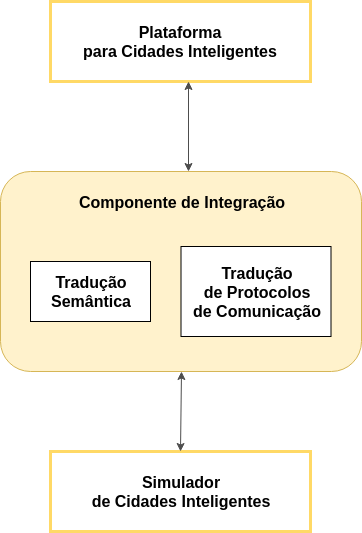
\includegraphics[width=0.4\textwidth]{figuras/integration-general-architecture.png}
	\caption{Arquitetura Proposta para Ambiente Integrado de Exerimentação de Plataformas de Cidades Inteligentes}
	\label{fig:general_architecture}
\end{figure}


Na Figura \ref{fig:general_architecture}, podemos ver os componentes presentes na arquitetura de integração do sistema aqui apresentada.
Como elucidado anteriormente, o componente de integração não pode possuir muitas responsabilidades, já que uma complexidade alta pode acarretar em um aumento expressivo no
tempo de transmissão dos dados, sendo esse um requisito importante para o sistema.
Já as ferramentas envolvidas, além de suas próprias funcionalidades, esperamos que as mesmas possuam um módulo de comunicação para suportar o fluxo de dados em tempo de execução.

O componente de integração tem a responsabilidade de solucionar os pontos mencionados anteriormente:

\begin{itemize}
    \item Tradução semântica entre o simulador e a plataforma

    \item Interoperação entre protocolos de rede

    \item Interferência mínima no tempo de envio e recebimento de dados
\end{itemize}

Como pode ser visto, o componente de integração tem como único objetivo atender requisitos não funcionais.
Ele deve tornar a comunicação do simulador e da plataforma transparente para ambos e adicionando a menor complexidade possível ao sistema.

Em resumo, devemos escolher ferramentas (simulador e plataforma) mais semelhantes possíveis, com o que diz respeito principalmente ao modelo conceitual e aos protocolos de
rede utilizados para comunicação; e implementar o componente de integração o mais simples possível, apenas com o objetivo de viabilizar a comunicação entre as ferramentas.

Para a validação da construção desse ambiente simulado de experimentação para plataformas de Cidades Inteligentes, usamos o simulador InterSCSimulator e a plataforma InterSCity,
sendo essas ferramentas desenvolvidas pelo nosso grupo de pesquisa. Ambas serão apresentadas a seguir, correlacionando os requisitos e a aquitetura de integração aqui
apresentada.

\subsection{InterSCSimulator}

O InterSCSimulator é um simulador de código aberto baseado em agentes para Cidades Inteligentes que oferece uma interface simples para definição de
cenários de larga escala \cite{santana_17}.
Pelo fato de ser possível configurar o tempo que dura um ciclo de simulação na ferramenta, ela já atende um dos \textbf{requisitos fundamentais}.
Com isso, podemos dizer que um ciclo de simulação é igual a um segundo real.
Como apresentado anteriormente, é necessário termos uma execução com noção de tempo real (um segundo de simulação igual a aproximadamente um segundo real) e permitir a
interferência em tempo de execução por terceiros para a construção desse ambiente integrado de experimentação.

Para atingir a escalabilidade mencionada, o InterSCSimulator foi implementado usando a linguagem \textit{Erlang}.
Essa é uma linguagem funcional que visa facilitar a implementação de aplicações de larga escala, paralelas e distribuídas.
Algumas características herdadas do modelo de atores, que é implementado pelo \textit{Erlang}, são: paralelismo, execução distribuída, tolerância a falhas e
protocolo de comunicação \cite{santana_17}.
Essa escalabilidade é importante para que possamos atender o \textbf{requisito fundamental} que diz respeito a capacidade de geração de grandes massas de dados
para a plataforma.
O InterSCSimulator é capaz de simular cenários com milhões de agentes executando simultaneamente, sendo assim possível simular cenários em uma escala realista para cidades de grande porte.

O InterSCSimulator foi implementado por Eduardo Zambom Santana, doutorando de nosso grupo de pesquisa, baseado no simulador de âmbito geral \textit{Sim-Diasca}.
A Figura \ref{fig:simulator_architecture} apresenta a sua arquitetura, onde, em azul, estão os diferentes tipos de agentes que podem existir no ambiente
simulado e, em vermelho, a definição dos cenários de Cidades Inteligentes, tudo isso sendo executado no topo do simulador \textit{Sim-Diasca}.

\begin{figure}[ht]
	\centering
	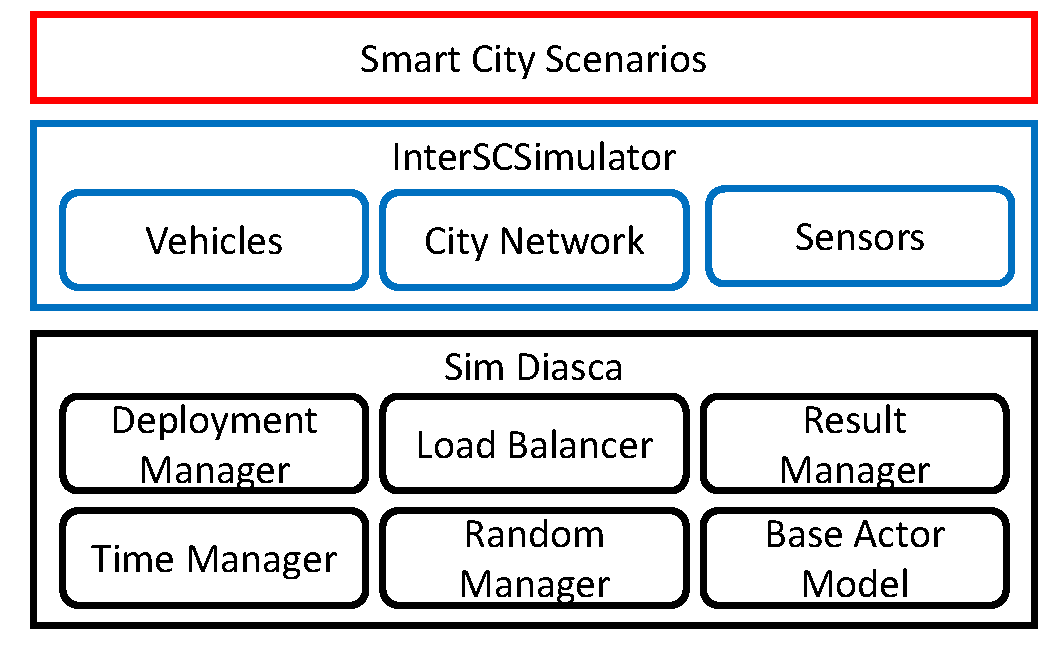
\includegraphics[width=0.5\textwidth]{figuras/Arquitetura.pdf}
	\caption{Arquitetura do InterSCSimulator}
	\label{fig:simulator_architecture}
\end{figure}

Fazendo um paralelo com um dos \textbf{requisito de integração} listados neste capítulo, cada \textit{Recurso} da cidade pode ser modelado como um agente da simulação.
Ou seja, um carro, uma vaga de estacionamento ou um ponto de parada de ônibus serão representados como agentes (caixas azuis na Figura \ref{fig:simulator_architecture})
na arquitetura do InterSCSimulator.
Na definição desses agentes especificamos o seu comportamento a cada passo da simulação.
Com isso, podemos especificar quais as \textit{Capacidades} de cada agente e adotar modelos aderentes com a realidade das cidades modernas.
O interessante dessa arquitetura baseada em agentes é o fato da implementação dos mesmos terem um grau de independência muito grande, onde é preciso apenas a definição
das mensagens que serão trocadas em tempo de execução.

Além disso, no contexto deste trabalho, foi adicionado um novo elemento a arquitetura da ferramenta para troca de dados com sistemas externos em tempo de execução,
sendo esse um dos \textbf{requisitos fundamentais e de integração} para obtermos um ambiente realista de experimentação.
Esse novo elemento nada mais é do que um novo agente onde o seu papel é receber e enviar mensagens de sensores e atuadores, seja no contexto de outros agentes ou de
outros sistemas.

Na implementação de um agente do InterSCSimulator podemos definir diversos comportamentos em diferentes momentos do seu cliclo de vida.
Podemos especificar o que será feito durante a sua criação, a sua destruição, a sua primeira ação na simulação e durante cada ciclo de execução.
Com isso, condições e caminhos dependentes do estado da simulação podem ser definidos para cada um dos tipos de agentes, flexibilizando a implementação dos
mais diversos modelos e formas de prover suas capacidades.
Essa liberdade para implementação de diversos comportamentos dos agentes nos permite usar modelos realistas e viabilizar as capacidades dos recursos no contexto das cidades,
atendendo mais um \textbf{requisito fundamental} e outro de \textbf{integração}.
Por exemplo, um carro após a sua partida em direção ao seu destino, calcula a cada ciclo de execução o fluxo de carros na via em que se encontra para o cálculo da
sua velocidade naquele instante, além de publicar a seu atual posição.
Nesse caso, podemos utilizar os mais diversos modelos matemáticos para calcular o fluxo de carros ou para determinar a sua velocidade, ao passo que a sua capacidade
de publicar sua localização georreferenciada também é atendida.

Na Figura \ref{fig:simulator_components}, são apresentados os componentes do simulador.
Inicialmente são passadas entradas para a simulação (arquivos XML) que em conjunto formam o cenário a ser simulado, esse cenário é executado e a
saída é criada com todos os eventos ocorridos na simulação.
A partir dessa saída existe a possibilidade de geração de uma visualização em um mapa ou através de gráficos.

\begin{figure}[ht]
	\centering
	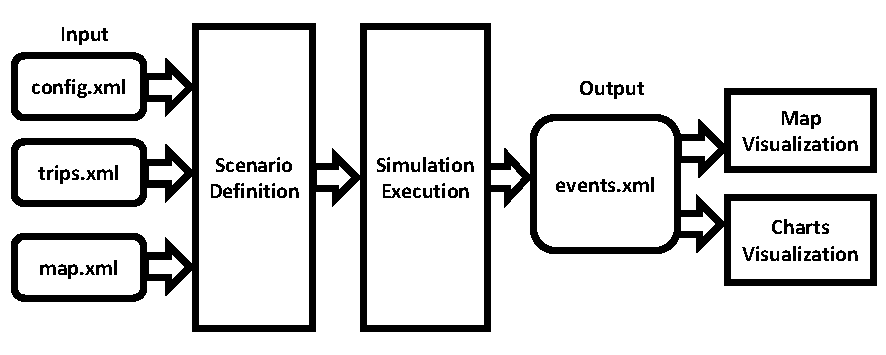
\includegraphics[width=0.7\textwidth]{figuras/Components.pdf}
	\caption{Componentes do InterSCSimulator}
	\label{fig:simulator_components}
\end{figure}

Como entrada, o InterSCSimulator recebe três arquivos XML. O \textit{config.xml} contém parâmetros da simulação, sendo eles o tempo total, o formato do
arquivo de saída e o caminho para o diretório contendo os outros arquivos de entrada e para geração do arquivo de saída.
O grafo representando a infraestrutura rodoviária da cidade é descrito no arquivo \textit{map.xml}, nesse grafo as vias são correspondentes as arestas e as esquinas entre
duas ou mais vias aos nós.
E por fim, as viagens a serem executadas são especificadas no arquivo \textit{trips.xml}, cada viagem contendo o seu tempo de início, modo de transporte, origem e destino.
Todas as ações realizadas pelos agentes são salvos no arquivo \textit{output.xml}, podendo haver quatro ações possíveis: 1) início de viagem, 2) saída de uma via,
3) entrada em uma via, e 4) chegada ao destino final.
O tempo, a localização e o modo de transporte utilizado pelo agente são registrados quando essas ações são salvas.

No trabalho desenvolvido por Eduardo Zambom Santana foi desenvolvido um simulador de larga escala, que é capaz de simular mais de 4 milhões de
agentes se movendo pela cidade de São Paulo~\cite{santana_17}.
Os modos de transportes suportados até então são: carro, ônibus, metrô e a pé.
Neste trabalho além de melhorias feitas nos modelos existentes, novos agentes foram adicionados ao simulador, além de agora ser possível a publicação e recebimento de
eventos em tempo de execução de maneira assícrona.

\subsection{Plataforma InterSCity}
\label{sec:interscity}

A plataforma InterSCity é um projeto de código aberto, baseado em microsserviços que visa permitir a pesquisa colaborativa, desenvolvimento e experimentos em Cidades
Inteligentes~\cite{arthur_17}.
A plataforma foi desenvolvida baseada em uma arquitetura de referência para plataformas de Cidades Inteligentes~\cite{santana_2016}, ela provê um conjunto de serviços
alto-nível baseado em nuvem para gerenciar recursos de \textit{IoT} heterogêneos~\cite{arthur_17}.

O projeto InterSCity visa atacar dois dos principais problemas arquiteturais no desenvolvimento de uma plataforma de alta qualidade que possa ser usada na prática no
contexto de Cidades Inteligentes: escalabilidade e evolução do software~\cite{arthur_17}.
Escalabilidade é necessária pelo fato da plataforma ter que interagir com um grande número de dispositivos \textit{IoT} espalhados pela cidade, milhões de usuários e
um grande tráfego de dados.
Como as cidades mudam constantemente, a questão da evolução é essencial, já que requisitos podem surgir ou mudar a qualquer momento, e adaptar a plataforma a fim de
incorporar novas funcionalidades não deve ser um empecilho.
Para resolver esses dois problemas apresentados, foram adotadas as seguintes estratégias~\cite{arthur_17}:

\begin{itemize}
	\item Modularidade via microsserviços
	\item Modelos e dados distribuídos
	\item Evolução descentralizada
	\item Reuso de projetos de software livre
	\item Adoção de padrões abertos
	\item Comunicação síncrona e assíncrona
	\item Serviços livres de estado
\end{itemize}

A Figura \ref{fig:platform_architecture} apresenta a arquitetura da plataforma InterSCSity.
Atualmente, ela é composta de 6 microsserviços:
\textit{Resource Adaptor}, oferece uma abstração para comunicação com os dispositivos \textit{IoT};
\textit{Data Collector}, responsável por coletar os dados dos sensores conectados;
\textit{Actuator Controller}, oferece uma interface para atuação junto aos dispositivos de \textit{IoT} com tais capacidades;
\textit{Resource Catalog}, possui dados estáticos dos recursos da cidade cadastrados;
\textit{Resource Discovery}, provê um serviço de descoberta de recursos;
e \textit{Resource Viewer}, disponibiliza uma visualização simples dos recursos da cidade. 

\begin{figure}[ht]
	\centering
	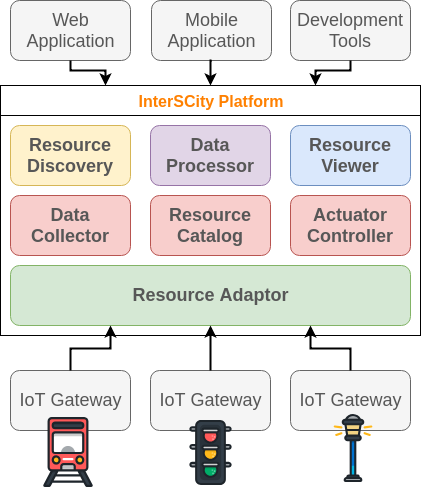
\includegraphics[width=0.5\textwidth]{figuras/platform_architecture.png}
	\caption{Arquitetura da plataforma InterSCity}
	\label{fig:platform_architecture}
\end{figure}

A comunicação entre esses microsserviços pode se dar de maneira síncrona ou assíncrona dependendo da situação.
A comunicação síncrona é feita via API \textit{Restful}, ou seja, requisições HTTP; e a assíncrona se dá via RabbitMQ\footnote{https://www.rabbitmq.com/}, uma implementação do protocolo AMQP.
O objetivo do protocolo AMQP é criar um padrão aberto para troca de mensagens assíncronas interoperável e de larga escala~\cite{vinoski_2006}.
A principal vantagem desse protocolo é permitir que o \textit{broker} de mensagens tome as decisões de roteamento, não necessitando a aplicação ter conhecimento
desse processo~\cite{vinoski_2006}.

A plataforma traz uma abstração chamada \textit{Resource}, que representa um recurso real da cidade, como ônibus, hospital, paradas de ônibus.
Cada um desses \textit{Resources} possuem \textit{Capabilities}, que pode ser de sensoriamento ou atuação, usualmente vinculados a algum tipo dispositivo \textit{IoT},
como capacidade de medir temperatura ou capacidade de mudar o estado de um semáforo.
Esses conceitos são os mesmos apresentados como requisitos para a construção de um ambiente integrado de experimentação para Cidades Inteligentes.
Como apresentado na seção anterior, semânticamente, esses recursos e capacidades aqui apresentados estarão associados a agentes e a definição de ações durante o seu
ciclo de vida no InterSCSimulator.

Na seção a seguir serão apresentados alguns exemplos de implementação da arquitetura aqui proposta utilizando o simulador InterSCSimulator e a plataforma InterSCity
para Cidades Inteligentes.

\section{Exemplos de Implementação}

Com o intuito de validar a arquitetura proposta foram implementados dois cenários de Cidades Inteligentes no ambiente integrado de experimentação.
Priorizamos implementar cenários de experimentação onde pudéssemos explorar todos os requisitos apresentados neste capítulo.

No primeiro cenário realizamos experimentos no contexto de estacionamento inteligente (conhecido com \textit{Smart Parking}), onde carros circulam pela cidade e ao
final do seu percurso procuram por uma vaga de estacionamento disponível mais próxima do seu destino, utilizando-se da plataforma para isso.
Nesse cenário, incluímos um novo agente à simulação e implementamos um mecanismo para publicação dos eventos ocorridos e requisição a serviços da plataforma em tempo real
e de forma assíncrona.

O segundo cenário de experimentação envolve o tráfego de carros inteligente através da utilização de Placas de Mensagens Variadas (PMVs) espalhadas pela cidade.
Nesse cenário a plataforma identifica trechos de maior trânsito e atua na cidade atualizando as mensagens apresentadas pelas PMVs em tempo real, notificando os
motoristas da lentidão no trecho, que por sua vez podem recalcular a sua rota evitando congestionamentos.
Para viabilizar esse experimento nos utilizamos das melhorias implementados no primeiro cenário, modificamos o modelo de trânsito para melhor se adequar a realidade e
implementamos o mecanismo de recebimento de comandos de atuação em tempo de execução.

Cada um desses cenários serão apresentados nas seções a seguir, de maneira a exemplificar a implementação da arquitetura proposta através da utilização do simulador
InterSCSimulator a a plataforma InterSCity para Cidades Inteligentes.

\subsection{Estacionamento Inteligente}
\label{sec:smart_parking}

Como foi apresentado, neste cenário de experimentação, simulamos motoristas realizando seus respoectivos percursos de carro e ao final procurando uma vaga disponível mais próxima ao
seu destino, provavelmente utilizando um aplicativo móvel que se comunica com a plataforma InterSCity.
Trazendo os conceitos de recursos da cidade e capacidades para esse cenário, temos os carros e as vagas de estacionamento sendo recursos, onde os carros são capazes de
fornecer a sua geolocalização (por exemplo via GPS) e as vagas de fornecer informação quanto a sua disponibilidade (por exemplo através de sensores infravermelho e uma
redes de sensores).

Esse cenário foi definido com o intuito de realizar experimentos envolvendo o serviço de descoberta de recursos da plataforma InterSCity.
Portanto, o aplicativo enviaria a posição do carro naquele momento, o seu destino final e o raio de busca, e a plataforma traria uma lista de vagas de estacionamento
disponíveis mais próximas.
Já no InterSCSimulator, foi necessário realizar algumas melhorias para que os \textbf{requisitos fundamentais} fossem atendidos.
Um novo agente para gerenciar as vagas de estacionamento da cidade, chamado \textit{Parking Controller}, foi implementado.
Esse agente possui a responsabilidade de gerenciar e armazenar dados referentes as vagas de estacionamento, e fazer a interface de comunicação com o componente de
integração que será apresentado mais adiante.
Além disso, modificamos o modelo de viagem do agente \textit{Carro}.
Anteriormente, o \textit{Carro} saia de uma origem e percorriar o seu trajeto até o destino, agora ao chegar próximo do seu destino ele requisita uma vaga disponível mais
próxima e se dirige até a mesma.
Com essas melhorias pudemos simular um cenário que se aproxima da realidade.

Para ilustrar o modelo descrito, a seguir será apresentado o ciclo de execução de um agente \textit{Carro} neste cenário:

\begin{enumerate}
    \item O agente \textit{Carro} é criado

    \item O caminho mais curto entre a origem e o destino é calculado

    \item O agente parte da sua origem no tempo determinado

    \item Ao chegar no nó anterior ao seu destino, uma vaga de estacionamento disponível é requisitada ao agente \textit{Parking Controller}

    \item Ao receber a vaga de estacionamento, o seu trajeto é recalculado em direção a mesma

    \item O agente se direciona e estaciona na vaga de estacionamento descoberta 
\end{enumerate}

Um fluxo alternativo a essa execução seria o carro modificar o seu percurso em direção da vaga de estacionamento (disponível até então), e ao chegar nela outro
carro a ter ocupado antes, sendo esse um caso comum nas grandes cidades.
Nesse caso, outra vaga de estacionamento é requisitada aumentando o seu raio de busca com o intuito de sempre encontrar vagas disponíveis.
Caso o agente do tipo carro necessitar realizar mais de três buscas de vagas disponíveis, o mesmo encerra a sua execução.

Quando o agente \textit{Carro} por fim estaciona em uma vaga disponível, o agente \textit{Parking Controller} é notificado e atualiza a sua estrutura de dados indicando
que a vaga foi ocupada pelo carro.
Além do mais, esse agente é responsável por atualizar o estado da vaga de estacionamento na plataforma.

Agora pensando nos \textbf{requisitos de integração}, o simulador precisa requisitar a plataforma em busca de vagas disponíveis mais próximas, e atualizar o estado
das vagas de estacionamento.
A plataforma InterSCity provê um \textit{API Restful} para comunicação com seus serviços (como o de descoberta de recursos), e o estado dos seus recursos podem ser
atualizados através da própria API ou via protocolo AMQP (\textit{Advanced Message Queuing Protocol}).
Esse levantamento é importante para a tomada de decisão de quais as responsabilidades e como será implementado o componente de integração.
Tendo em vista que a complexidade do componente de integração deve ser a menor possível, e a não existência de um meio de publicação de eventos em tempo de execução
no InterSCSimulator, decidimos utilizar o RabbitMQ (implementação do protocolo AMQP) na implementação desse novo meio de comunicação.
Com isso, o simulador poderia atualizar o estado das vagas diretamente na plataforma de forma assíncrona, sem necessidade de auxílio do componente de integração.
As requisições HTTP feitas ao serviço de descoberta da plataforma seriam feitas pelo componente de integração, principalmente pelo fato de requisições HTTP serem
síncronas, o que poderia travar a simulação na espera por uma resposta.

Para facilitar o entendimento da integração realizada, dividiremos a explicação em duas partes: a primeira visando a requisição de vagas disponíveis mais próximas
do carro ao serviço de descoberta da plataforma InterSCity; e a segunda apresentado o fluxo de atualização do estado de uma vaga de estacionamento (ocupada
ou disponível) baseada na emulação.

A Figura \ref{fig:descoberta} apresenta a integração realizada para utilização do serviço de descoberta provido pela plataforma InterSCity.
O componente de integração foi chamado de \textit{Parking Spot Discoverer}, e foi implementado como um agente Erlang que consegue se comunicar com os agentes da
simulação via troca de mensagens.
O uso do componente de integração se fez necessário para que a simulação exerça a carga que aplicações exerceriam utilizando o protocolo HTTP para acessar
a \textit{API Restful}.
Como dito, requisições HTTP são síncronas, e a realização das mesmas dentro da simulação atrasaria consideravelmente a sua finalização, já que bloquearia a
execução dos agentes enquanto aguardariam a resposta da plataforma.
Antes de chegarmos a tal solução implementamos uma versão onde o próprio simulador realizava requisições HTTP para a plataforma em tempo de execução, entretanto,
essa solução gerou um enorme gargalo.
Descrevemos abaixo o fluxo de atividades apresentado na Figura \ref{fig:descoberta}.

\begin{enumerate}
    \item Ao chegar um nó antes do seu destino, o \textit{Car} solicita a vaga de estacionamento para o agente \textit{Parking Controller}, passando a sua
	localização como parâmetro.

	\item O agente \textit{Parking Controller} então envia a localização para o \textit{Parking Spot Discoverer} que solicita a vaga disponível mais próxima,
	em um raio de 500 metros.

	\item O \textit{Parking Spot Discoverer} faz uma requisição HTTP para o serviço de descoberta da plataforma que retorna a vaga em questão.
	Caso não seja encontrada uma vaga disponível (não ocupada) em um raio de 500 metros, esse raio é multiplicado por dois até que se encontre uma vaga
	disponível.

	\item O identificador da vaga é retornado para o agente \textit{Parking Controller} e ele marca a vaga como utilizada em uma estrutura de dados mantida no simulador.

    \item O identificador da vaga é recebido pelo agente \textit{Car} e a rota é recalculada para chegar até ela.
\end{enumerate}

\begin{figure}[ht]
	\centering
	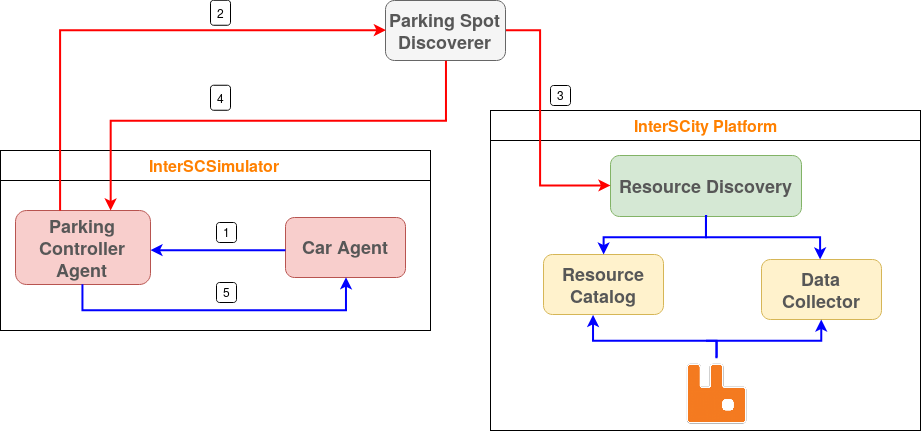
\includegraphics[width=\textwidth]{figuras/integration_get_data_smart_parking.png}
	\caption{Integração para descoberta de vagas livres próximo do destino da
	viagem}
	\label{fig:descoberta}
\end{figure}

A Figura \ref{fig:atualizacao} apresenta a integração realizada com o intuito de atualizar o estado das vagas de estacionamento na plataforma baseado nos
acontecimentos da simulação.
Como foi adicionado a funcionalidade de publicação dos eventos da simulação via RabbitMQ para os interessados, não foi necesário a utilização do
componente de integração, já que a plataforma também utiliza o mesmo protocolo para divulgação dos seus dados entre microsserviços.
O fluxo apresentado na Figura \ref{fig:atualizacao} contém os seguintes passos.

\begin{enumerate}
    \item O agente \textit{Car} estaciona na vaga de estacionamento e notifica o \textit{Parking Controller}.

	\item O \textit{Parking Controller} informa, via \textit{RabbitMQ}, que a vaga está ocupada usando o seu identificador.

	\item O \textit{RabbitMQ} repassa esse dado para os microsserviços \textit{Resource Catalog} e \textit{Data Collector}.
\end{enumerate}

\begin{figure}[ht]
	\centering
	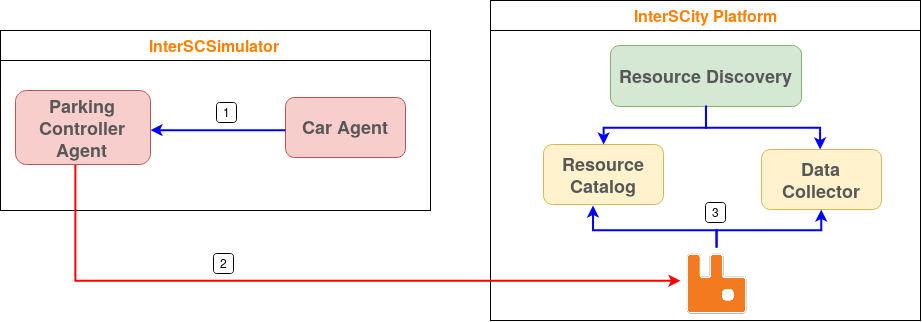
\includegraphics[width=\textwidth]{figuras/integration_publish_data_smart_parking.png}
	\caption{Integração para publicar dados}
	\label{fig:atualizacao}
\end{figure}

Vale ressaltar que as atividades 2 e 3 apresentadas na Figura \ref{fig:atualizacao} também são executadas quando a vaga é liberada.
Após dez minutos que o agente está estacionado na vaga, o agente \textit{Parking Controller} libera a vaga na estrutura de dados mantida dentro do simulador e informa o
ocorrido para a plataforma.
Com isso, a plataforma atualiza os dados da vaga tanto quando ela é ocupada quando liberada.

Após a implementação da arquitetura descrita, fomos capazes de executar experimentos de larga escala no contexto de estacionamento inteligente.
Os resultados obtidos serão apresentados no próximo capítulo.

Todavia, não exercitamos todos os requisitos apresentados para a construção de um ambiente simulado e integrado para experimentação de plataformas de Cidades Inteligentes.
Por isso, implementamos um segundo cenário de Cidades Inteligentes onde, por exemplo, a atuação no ambiente simulado se fez necessária.


\subsection{Tráfego de Carros Inteligente}
\label{sec:smart_traffic}

Com o objetivo de exercitar o envio de comandos de atuação da plataforma para o ambiente simulado, que não foi explorado no cenário de estacionamento inteligente apresentado
anteriormente, definimos um novo cenário.
Neste cenário, visamos identificar trechos em vias da cidade com tráfego de carros anômalo (devido ao fechamento de ruas, acidentes, desastres naturais e etc.) e notificar
previamente os motoristas para evitarem passar naquele trecho através de Placas de Mensagens Variadas (PMVs).
Consideramos aqui uma anomalia uma variação considerável na velocidade média dos carros que trafegam naquele trecho de via naquele horário.
Essas PMVs são posicionadas em pontos estratégicos da cidade e apresentam alertas aos motoristas em tempo real sobre possíveis anomalias no trânsito, e com isso motoristas
podem mudar o seu percurso evitando maiores congestionamentos na cidade.

Essencialmente, esse cenário funciona da seguinte forma:

\begin{enumerate}
    \item A plataforma coleta dados históricos de carros para definir limiares (\textit{thresholds}) de velocidade média para cada trecho de via da cidade em cada horário.
        Para isso, o ambiente simulado envia dados de posicionamento georreferenciado dos carros a cada ciclo de execução, simulando por exemplo um dispositivo que contem um
        sistema de GPRS (\textit{General Packet Radio Service}) + GPS (\textit{Global Positioning System}).
        Com uma série de pontos de onde o carro passou em cada instante, se torna possível calcular a velocidade média do mesmo, logo obtemos a velocidade média de carros
        que passaram naquele trecho naquele dado momento durante todo o dia.
        Tendo esses limiares, a plataforma se torna capaz de identificar anomalias na velocidade média dos carros em tempo real, verificando se a variação naquele instante
        extrapola ou não o que foi identificado com os dados históricos.

    \item Ao identifiar uma anomalia de trânsito em algum trecho, a plataforma identifica as PMVs mais próximas do incidente e atualiza a sua mensagem informando os motoristas
        do ocorrido.

    \item Caso o motorista passe por uma PMV contendo essa mensagem, ele verifica se o trecho mencionado faz parte do seu percurso. Sendo verdade, o mesmo recalcula a sua
        rota evitando maiores congestionamentos na região.
\end{enumerate}

Nesse cenário de experimentação, o novo serviço de processamento de dados (históricos e de tempo real), que está em desenvolvimento, e o envio de comandos de atuação da plataforma
InterSCity puderam também ser testados.
Além disso, foi possível finalizar a validação da arquitetura proposta para a criação de um ambiente para experimentação em plataformas de Cidades Inteligentes,
implementando a atuação em tempo real no ambiente simulado.

Para realizar experimentos envolvendo essas funcionalidades da plataforma InterSCity, foi necessário implementar o conceito de PMVs, eventos de fechamentos de via e de
processamento de comandos de atuação em tempo de execuação no InterSCSimulator.
Além do mais, foi utilizada a publicação de eventos (dados de sensores) implementado para o cenário anterior, já que para o funcionamento do serviço de processamento de dados
em tempo real da plataforma precisamos enviar a cada ciclo de execução da simulação o posicionamento de todos os carros presentes.
Sendo essas melhorias necessárias para atender os \textbf{requisitos fundamentais} para esse cenário.

O modo de publicação de dados em tempo de execução no InterSCSimulator foi refatorado para melhor atender ambos os cenários implementados.
Como visto no cenário anterior, a publicação de eventos da simulação se dava através do agente \textit{Parking Controller} (como pode ser visto na Figura \ref{fig:atualizacao}), já que
até então o único tipo de evento publicado pelo simulador era a atualização da disponibilidade de uma vaga de estacionamento.
No intuito de permitir que outros agentes da simulação também pudessem publicar os seus eventos, um novo agente chamado \textit{Publisher} foi criado, removendo essa responsabilidade
anteriormente atribuída ao agente \textit{Parking Controller}.
Desse modo, o agente do tipo carro também se tornou capaz de publicar a sua posição, onde agora a cada ciclo de execução é enviada uma mensagem a um agente \textit{Publisher}
contendo sua localização.

Visando tornar factível a simulação de eventos de fechamento de vias na cidade, adicionamos o conceito de eventos de trânsito ao InterSCSimulator.
Um novo arquivo de entrada para o simulador e um novo agente foram adicionados.
O novo arquivo de entrada (chamado por padrão \textit{events.xml}), contem uma lista de eventos de fechamento de via que serão agendados na simulação.
Como pode ser visto na Listagem \ref{code:events} abaixo, cada evento é representado da seguinte forma:
(i) o tipo do evento de trânsito;
(ii) a via a ser fechada (uma aresta no grafo da cidade);
(iii) o momento de início do evento;
(iv) a duração do evento;
(v) a porcentagem da capacidade do fluxo de carros que ainda estará em funcionamento, usada no caso de um fechamento parcial do trecho.
O novo agente chamado \textit{Events Manager} é responsável por agendar todos esses eventos no início da simulação e alterar o grafo da cidade no momento programado.
Quando o trecho da via é fechado, a aresta do grafo da cidade é removida momentaneamnte até o evento ser encerrado, impedindo assim a possibilidade de passagem de qualquer
carro.
Agora quando o evento apenas reduz a capacidade de fluxo de carros da via, modificamos a sua capacidade para atender o que foi programado até o evento ser encerrado,
onde essa capacidade é um atributo dado àquela aresta do grafo.

\lstset{
    language=xml,
    tabsize=3,
    frame=lines,
    caption=Arquivo de entrada contendo os eventos de fechamento de vias,
    label=code:events,
    frame=shadowbox,
    rulesepcolor=\color{gray},
    xleftmargin=20pt,
    framexleftmargin=15pt,
    keywordstyle=\color{blue}\bf,
    commentstyle=\color{OliveGreen},
    stringstyle=\color{red},
    numbers=left,
    numberstyle=\tiny,
    numbersep=5pt,
    breaklines=true,
    showstringspaces=false,
    basicstyle=\footnotesize,
    emph={uuid,node},emphstyle={\color{magenta}}}
    \lstinputlisting{files/events.csv}

Para a representação das PMVs no InterSCSimulator, foi criado um agente chamado \textit{PMV Manager} onde o seu papel era atualizar as mensagens de PMVs.
As PMVs em si foram implementadas como atributos de vértices do grafo da cidade (sendo os vértices o encontro de duas ou mais vias), onde nesse atributo é guardada uma lista
de trechos de vias (arestas) onde foram encontradas alguma anomalia no trânsito.
Os agentes do tipo carro ao passar por um vértice que continha esse atributo, verificavam se alguma das arestas ali presentes faziam parte do seu trajeto ou não.
Caso positivo, o seu percurso era recalculado, caso contrário o mesmo se mantinha inalterado.

E a última implementação no InterSCSimulator necessária para atender os requisitos apresentados seguindo a arquitetura proposta foi o recebimento de comandos de atuação e
processamento dos mesmos em tempo de execuação.
Sendo essa uma funcionalidade fundamental para a atualização das PMVs em tempo de execução pela plataforma.
Diante disso, mais um novo agente foi criado para ficar a espera desses comandos enviados pela plataforma, sendo ele chamado de \textit{Listener}.
Como um comando de atuação pode ser enviado a qualquer momento, foi necessário esse novo agente, cuja única responsabilidade é receber esse comando e armazená-lo em uma
estrutura de dados, para que outros agentes não ficassem bloqueados (bloqueando também a simulação) a espera de tal acontecimento.
Ou seja, esse agente fica em um laço (\textit{loop}) infinito a espera de uma mensagem que é enviada via AMQP (mesmo protocolo utilizado para publicação dos dados).
A utilização do RabbitMQ foi escolhida devido a possibilidade da plataforma InterSCity enviar comandos de atuação através do mesmo, e como foi uma funcionalidade nova
decidimos utilizar a mesma tecnologia, reduzindo assim o problema de interoperabilidade discutido neste capítulo.
Quando um comando é recebido, no caso uma aresta de trecho anômalo a ser atualizada em uma PMV, ele armazena essa mensagem em uma estrutura de dados que será acessada no
próximo ciclo de execução pelo \textit{PMV Manager}, que por sua vez atualizará a atributo da referida PMV (vértice no grafo).

Após a apresentação das funcionalidades e melhorias implementadas, as duas vias de fluxo de comunicação entre o simulador e a plataforma serão apresentados a seguir.
Na Figura \ref{fig:smart_traffic_publish_data}, o passo a passo para a publicação dos dados de posicionamento de cada um dos carros a cada ciclo de execução é exposto.

\begin{figure}[ht]
	\centering
	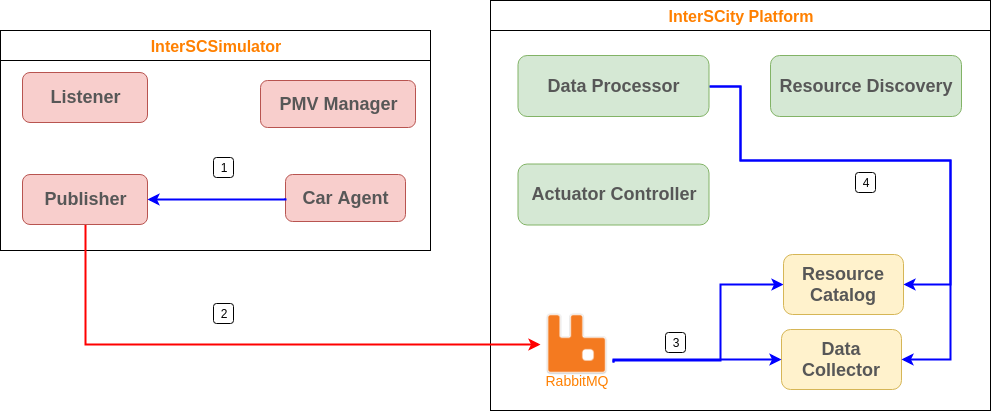
\includegraphics[width=\textwidth]{figuras/integration-publish-car-position.png}
	\caption{Integração para publicar dados de posicionameto de carros}
	\label{fig:smart_traffic_publish_data}
\end{figure}

\begin{enumerate}
    \item O agente do tipo carro a cada ciclo de execução envia uma mensagem para o agente \textit{Publisher} contendo a sua posição naquele dado momento.

    \item O agente \textit{Publisher} se conecta ao \textit{broker} do RabbitMQ e publica uma mensagem contendo: o identificador do carro, o seu posicionamento, e o \textit{timestamp}.

    \item Os microsserviços \textit{Resource Catalog} e \textit{Data Collector} são notificados e recebem tais dados. O \textit{Resource Catalog} atualiza o último dado monitorado
        daquele carro, e o \textit{Data Collector} atualiza a sua base de dados contendo todas as medições.

    \item O microsserviço \textit{Data Processor} acessa dados armazenados por esses outros serviços com o intuito de definir limiares para velocidade média de vias (dados históricos),
        ou para identificar anomalias no trânsito (fluxo de dados em tempo real).
\end{enumerate}

Já na Figura \ref{fig:smart_traffic_actuation}, é apresentado o fluxo para atualização da lista de trechos anômalos de vias em PMVs, representando aqui um comando de atuação no
ambiente simulado.
Lembrando que o gatilho para a execução desse processo é o serviço de processamento de dados identificar alguma anomalia no trânsito.

\begin{figure}[ht]
	\centering
	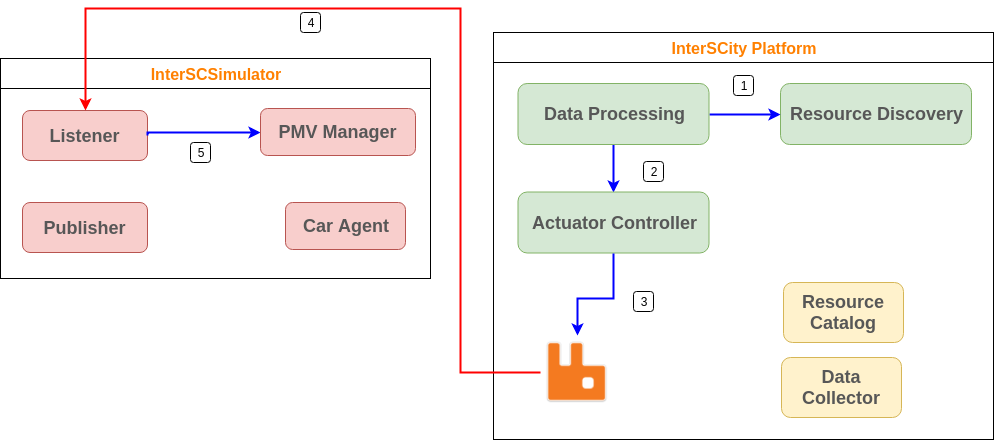
\includegraphics[width=\textwidth]{figuras/integration-actuate-pmv.png}
	\caption{Integração para atuação em Placas de Mensagens Variadas}
	\label{fig:smart_traffic_actuation}
\end{figure}

\begin{enumerate}
    \item O \textit{Data Processor} ao identificar uma anomalia no trânsito em determinado ponto da cidade, ele requisita para o \textit{Resource Discovery} as PMVs mais próximas
        daquele ponto, para que as mesmas possam ser atualizados.

    \item Ao serem identificados as PMVs, o \textit{Data Processor} envia os identificadores das PMVs e do trecho anômalo para o \textit{Actuator Controller}.

    \item O \textit{Actuator Controller} formata essas mensagens e publica as mesmas em um dos canais do RabbitMQ.

    \item O agente \textit{Listener}, cujo único papel é esperar por esse tipo de mensagem, recebe a mesma e a armazena em uma estrutura de dados compatilhada pelos agentes do simulador.

    \item O agente \textit{PMV Manager} verifica a presença dessa nova mensagem na estrutura de dados compatilhada, e atualiza o atributo que representa a PMV no vértice do grafo
        viário da cidade, adicionado mais esse trecho para a lista presente ou criando-a caso não existe nenhum outro trecho.
\end{enumerate}

Um ponto interessante desse segundo cenário, foi a não necessidade de um componente de integração, já que ambas as ferramentas se comunicam através do mesmo protocolo (inclusive a
mesma ferramenta) e conseguem representar os mesmos conceitos de maneira equivalente.
Esse é o cenário ideal para criação de um ambiente simulado de experimentação para uma plataforma de Cidades Inteligentes, já que não foi essencial a implementação desse
componente extra, que como discutido traria mais complexidade para o sistema, podendo aumentar o tempo de resposta entra as ferramentas.
Claro que tudo isso foi possível porque neste mesmo trabalho fizemos toda a implementação dos \textbf{requisitos fundamentais} apresentados, portanto,
tivemos a oportunidade de tomar as decisões técnicas que facilitaram a integração entra as duas ferramentas.

No capítulo a seguir, serão apresentados alguns resultados experimentais baseados na implementação desse cenário de tráfego de carros inteligente.

\section{Discussão}

Durante a implementação dos dois cenários de Cidades Inteligentes apresentados, algumas adversidades foram encontradas e solucionadas.
A fim de contribuir com trabalhos futuros que sigam a solução aqui proposta, uma discussão sobre os principais problemas e dificuldades encontradas será feita
nesta seção.
O intuito aqui é enfatizar os principais obstáculos a serem enfrentados durante a implementação de novos cenários no ambiente integrado usando o simulador InterSCSimulator e
a plataforma InterSCity ou até mesmo envolvendo outras ferramentas.

Como vem sendo discutido no decorrer deste trabalho, a integração de ferramentas não é algo trivial.
Apesar de tanto o simulador quanto a plataforma utilizada serem voltados para o contexto de Cidades Inteligentes, na maioria das vezes, elas não foram concebidas inicialmente
para serem integradas com ferramentas de outra natureza.
Através dos próprios requisitos apresentados podemos antever o maior desafio a ser enfrentado: a interoperabilidade.
Interoperabilidade essa tanto a nível de comunicação e quanto semanticamente.

Como constatado na implementação dos dois cenários apresentados, tentamos ao máximo reduzir a responsabilidade do componente de integração, que ao ser atribuído muitas
tarefas pode se tornar um problema.
Tanto que não foi necessária a implementação desse componente no segundo cenário apresentado, tendo em vista que as ferramentas já atendiam os requisitos de integração.
Isso pode ser atribuído ao fato de ambas as ferramentas (InteSCSimulator e InterSCity) serem mantidas pelo nosso grupo de pesquisa, onde tivemos a liberdade de evoluir o
que foi preciso nas próprias ferramentas para facilitar a integração.
Em um contexto onde não existe essa flexibilidade o desafio se tornario bem mais complexo.

Mesmo assim, enfrentamos problemas principalmente com a escalabilidade da solução.
Em experimentos anteriores e isolados, foi demonstrado que ambas as ferramentas eram escaláveis, se comportando bem diante de uma grande carga de trabalho.
Entretanto, a integração traz alguns elementos extras que por menor que sejam interferem em cenários de larga escala.
Em experimentos na escala de uma cidade como São Paulo, qualquer mínimo detalhe é potencializado.
Semanticamente não tivemos muitos problemas, já que ambas as ferramentas foram implementadas seguindo conceitos similares, devido a própria sinergia do grupo de
pesquisa.
Todavia, a comunicação entre as ferramentas foi a raíz da maior parte dos problemas enfrentados.

Por exemplo, inicialmente, tentamos realizar qualquer interação com a plataforma através de requisições HTTP, usando a sua API \textit{Restful}.
Contudo, percebemos que o componente de integração necessitaria de uma complexidade muito maior para tratar todas essas requisições paralelamente sem se tornar um
gargalo para o sistema.
Por isso, decidimos explorar bastante o protocolo AMQP através da implementação do RabbitMQ.
Essa se apresentou uma solução mais simples, já que o \textit{broker} do RabbitMQ trata todas essas questões de escalabilidade de maneira bem eficiente, sendo essa
uma solução adotada pelo mercado.
Além do mais, pelo fato da comunicação via AMQP ser assíncrona e pela própria natureza dos cenários implementados, diferente de requisições HTTP, ela se apresentou uma
solução mais adequada, não bloqueando agentes da simulação a espera de respostas.
Logo, sempre que possível, transferir responsabilidades para ferramentas de terceiros comprovadamente capazes de atender os requisitos ao invés de implementar a sua
própria solução é desejável.

Nesse processo de melhoria da escalabilidade da solução integrada, várias mudanças foram feitas em ambas as ferramentas.
Foram encontrados problemas de escalabilidade antes não evidenciados por outros experimentos isolados, demonstrado que a solução de ambiente para experimentação para
plataformas de Cidades Inteligentes atingiu seus objetivos, apontando melhorias nos sistemas que só seriam evidenciadas ao enfrentar cargas de trabalho à nível de uma
cidade como São Paulo.

A nível da plataforma InterSCity, implementações envolvendo técnicas para armazenamento em cache de dados mais utilizados foram feitas.
Ademais, melhorias envolvendo a automatização da implantação do plataforma foram realizadas.
Já no InterSCSimulator, encontramos alguns problemas na implementação dos modelos apresentados que causaram problemas de escalabilidade.
Ou seja, dependendo do cenário e de como foi implementado, apenas reduzir a complexidade do componente de integração (até mesmo a não existência) ainda não é a solução.
Portanto, poder modificar as próprias ferramentas é algo interessante, haja vista que a forma que os modelos, métodos e funcionalidades foram implementados podem não
ter sido testados em ambientes de estresse, tornando-se gargalos durante experimentos de larga escala.

Isso evidencia a importância da utilização de ferramentas livres para a construção de ambientes de experimentação para plataformas de Cidades Inteligentes.

\par

\chapter{Estudos de Caso}
\label{cap:estudos-de-caso}

%Explicar o porque de cada cenário
%Detalhar implementação e experimentos realizados:

Com o intuito de validar a arquitetura proposta foram realizados dois estudos de caso envolvendo diferentes cenários de Cidades Inteligentes em um ambiente simulado de experimentação.
Priorizamos implementar cenários de experimentação onde pudéssemos explorar todos os requisitos apresentados no Capítulo \ref{cap:proposta}.
Através desses dois experimentos, pudemos validar a solução apresentada para construção de um ambiente simulado de experimentação para plataformas de Cidades Inteligentes.
Foi possível exercitar as principais funcionalidades necessárias para a realização de experimentos desse tipo, através da integração do InterSCSimulator e a plataforma InterSCity.

No primeiro cenário, realizamos experimentos no contexto de estacionamento inteligente (conhecido com \textit{Smart Parking}), onde carros circulam pela cidade e, ao
final do seu percurso, procuram por uma vaga de estacionamento disponível mais próxima do seu destino, utilizando-se da plataforma para isso.
Nesse cenário, incluímos um novo agente à simulação e implementamos um mecanismo para publicação dos eventos ocorridos e requisição a serviços da plataforma em tempo real
e de forma assíncrona.

O segundo cenário de experimentação envolve o tráfego de carros inteligente através da utilização de Placas de Mensagens Variadas (PMVs) espalhadas pela cidade.
Nesse cenário, a plataforma identifica trechos de maior trânsito e atua na cidade atualizando as mensagens apresentadas pelas PMVs em tempo real, notificando os
motoristas da lentidão no trecho, que por sua vez podem recalcular a sua rota evitando congestionamentos.
Para viabilizar esse experimento fizemos uso das melhorias implementadas no primeiro cenário acrescidas de outras tais como: modificação do modelo de trânsito para melhor se adequar a realidade e
implementação do mecanismo de recebimento de comandos de atuação em tempo de execução.

A seguir a arquitetura do simulador InterSCSimulator e da plataforma InterSCity serão apresentadas, haja vista que essas foram as ferramentas utilizadas para o desenvolvimento
dos estudos de caso.
Além disso, cada um dos cenários de Cidades Inteligentes mencionados serão apresentados detalhadamente, visando exemplificar a implementação da arquitetura proposta e os resultados experimentais obtidos.
Ao final, realizaremos uma análise crítica sobre os resultados obtidos, apontando possíveis melhorias a serem feitas.

\section{Ferramentas}

O simulador InterSCSimulator e a plataforma InterSCity serão detalhados quanto as suas respectivas arquiteturas.
Faremos uma discussão de como os \textbf{requisitos fundamentais e de integração} apresentados no Capítulo \ref{cap:proposta} serão atendidos em cada ferramenta.

\subsection{InterSCSimulator}

O InterSCSimulator é um simulador de código aberto baseado em agentes para Cidades Inteligentes que oferece uma interface simples para definição de
cenários de larga escala \citep{santana_17}.
Pelo fato de ser possível configurar o tempo que dura um ciclo de simulação na ferramenta, ela já atende um dos \textbf{requisitos fundamentais} descritos na Seção \ref{sec:requisitos}.
Com isso, podemos dizer que um ciclo de simulação é igual a um segundo real.
É sabido que é necessário termos uma execução com noção de tempo real (um segundo de simulação igual a aproximadamente um segundo real) e permitir a
interferência em tempo de execução por terceiros para a construção desse ambiente integrado de experimentação.

Para atingir a escalabilidade mencionada, o InterSCSimulator foi implementado usando a linguagem \textit{Erlang}.
Essa é uma linguagem funcional que visa facilitar a implementação de aplicações de larga escala, paralelas e distribuídas.
Algumas características herdadas do modelo de atores, que é implementado pelo \textit{Erlang}, são: paralelismo, execução distribuída, tolerância a falhas e
protocolo de comunicação \citep{santana_17}.
Essa escalabilidade é importante para que possamos atender o \textbf{requisito fundamental} que diz respeito à capacidade de geração de grande massa de dados
para a plataforma.
O InterSCSimulator é capaz de simular cenários com milhões de agentes executando simultaneamente, possibilitando trabalhar-se em uma escala realista para cidades de grande porte.

O InterSCSimulator foi implementado por Eduardo Zambom Santana, doutorando do nosso grupo de pesquisa, baseado no simulador de âmbito geral \textit{Sim-Diasca}.
A Figura \ref{fig:simulator_architecture} representa a sua arquitetura da seguinte forma: em azul estão os diferentes tipos de agentes que podem existir no ambiente
simulado e, em vermelho a definição dos cenários de Cidades Inteligentes.
Tudo isso sendo executado no topo do simulador \textit{Sim-Diasca}.

\begin{figure}[ht]
	\centering
	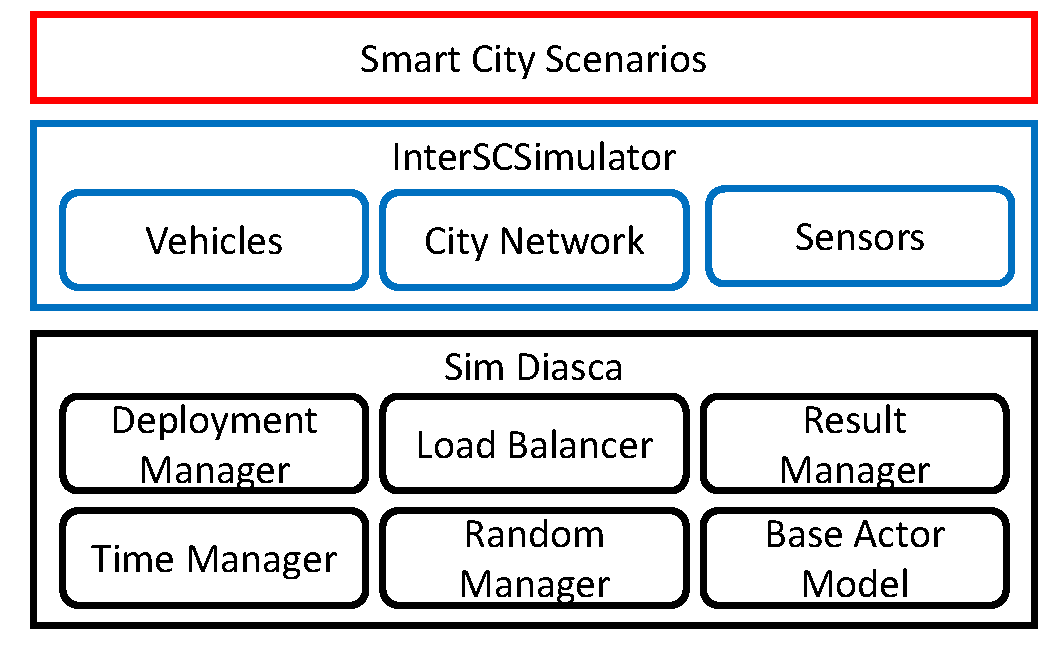
\includegraphics[width=0.5\textwidth]{figuras/Arquitetura.pdf}
	\caption{Arquitetura do InterSCSimulator}
	\label{fig:simulator_architecture}
\end{figure}

Fazendo um paralelo com um dos \textbf{requisitos de integração}, cada \textit{Recurso} da cidade pode ser modelado como um agente da simulação, ou seja, um carro, uma vaga de estacionamento ou um ponto
de parada de ônibus serão representados como agentes (caixas azuis na Figura \ref{fig:simulator_architecture}).
Na definição desses agentes especificamos o seu comportamento a cada passo da simulação.
Com isso, podemos descrever quais as \textit{Capacidades} de cada agente e adotar modelos compatíveis com a realidade das cidades modernas.
Por exemplo, podemos determinar que um agente do tipo carro envie sua localização a cada passo da simulação e que ele recalcule a sua rota apenas quando deparado com uma PMV.
O interessante dessa arquitetura baseada em agentes é o fato da sua implementação ter um alto grau de independência, onde é preciso apenas a definição das mensagens que serão trocadas em tempo
de execução.

No contexto desta dissertação, foi adicionado um novo elemento à arquitetura da ferramenta para troca de dados com sistemas externos em tempo de execução,
sendo esse um dos \textbf{requisitos fundamentais e de integração} para obtermos um ambiente realista de experimentação.
Esse novo elemento nada mais é do que um novo agente, cujo papel é receber e enviar mensagens de sensores e atuadores, seja no contexto de outros agentes ou de outros sistemas.

Na implementação de um agente do InterSCSimulator, podemos definir diversos comportamentos em diferentes momentos do seu cliclo de vida.
É possível especificar o que será feito durante a sua criação, a sua destruição, a sua primeira ação na simulação e durante cada ciclo de execução.
Com isso, condições e caminhos dependentes do estado da simulação podem ser definidos para cada um dos tipos de agentes, flexibilizando a implementação dos
mais diversos modelos e formas de prover suas capacidades.
Essa liberdade para implementação de diversos comportamentos dos agentes nos permite usar modelos realistas e viabilizar as capacidades dos recursos no contexto das cidades,
atendendo aos \textbf{requisitos fundamentais e de integração}.
Por exemplo, um carro, após a sua partida em direção ao seu destino, calcula a cada ciclo de execução o fluxo de carros na via em que se encontra para o cálculo da
sua velocidade naquele instante, além de publicar a sua posição atual.
Nesse caso, podemos utilizar os mais diversos modelos matemáticos para calcular o fluxo de carros ou para determinar a sua velocidade, ao passo que a sua capacidade
de publicar sua localização georreferenciada também é atendida.

Na Figura \ref{fig:simulator_components}, são apresentados os componentes do simulador.
Inicialmente são dadas entradas para a simulação (arquivos XML) que em conjunto formam o cenário a ser simulado.
Esse cenário é executado e a saída é criada com todos os eventos ocorridos na simulação.
A partir dessa saída, existe a possibilidade de geração de uma visualização em um mapa ou através de gráficos.

\begin{figure}[ht]
	\centering
	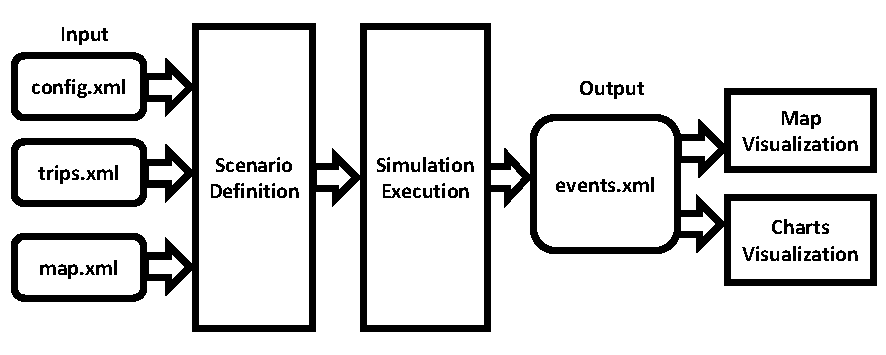
\includegraphics[width=0.7\textwidth]{figuras/Components.pdf}
	\caption{Componentes do InterSCSimulator}
	\label{fig:simulator_components}
\end{figure}

Como entrada, o InterSCSimulator recebe três arquivos XML.
O \textit{config.xml} contém parâmetros da simulação: o tempo total, o formato do
arquivo de saída e o caminho para o diretório contendo os outros arquivos de entrada e para geração do arquivo de saída.
O grafo representando a infraestrutura rodoviária da cidade é descrito no arquivo \textit{map.xml}: as vias são representadas pelas arestas e as esquinas entre
duas ou mais vias pelos nós.
Por fim, as viagens a serem executadas são especificadas no arquivo \textit{trips.xml}, cada viagem contendo o seu tempo de início, modo de transporte, origem e destino.
Todas as ações realizadas pelos agentes são salvas no arquivo \textit{output.xml}, podendo haver quatro ações possíveis: 1) início de viagem, 2) saída de uma via,
3) entrada em uma via, e 4) chegada ao destino final.
O tempo, a localização e o modo de transporte utilizado pelo agente são registrados quando essas ações são salvas.

Os modos de transportes suportados até o momento são: carro, ônibus, metrô e a pé.
Neste trabalho, além de melhorias feitas nos modelos existentes, novos agentes foram adicionados ao simulador, além da nova possibilidade de publicação e o recebimento de
eventos em tempo de execução de maneira assíncrona.

\subsection{Plataforma InterSCity}
\label{sec:interscity}

A plataforma InterSCity é um projeto de código aberto, baseado em microsserviços que visa permitir a pesquisa colaborativa, desenvolvimento e experimentos em Cidades
Inteligentes~\citep{arthur_17}.
A plataforma foi desenvolvida baseada em uma arquitetura de referência para plataformas de Cidades Inteligentes~\citep{santana_2016}, ela provê um conjunto de serviços de
alto-nível baseado em nuvem para gerenciar recursos de IoT heterogêneos.

O InterSCity visa solucionar dois dos principais problemas arquiteturais no desenvolvimento de uma plataforma de alta qualidade que possa ser usada na prática, no
contexto de Cidades Inteligentes: escalabilidade e evolução do software~\citep{arthur_17}.
Escalabilidade é necessária pelo fato da plataforma ter que interagir com um grande número de dispositivos IoT espalhados pela cidade, milhões de usuários e
um grande tráfego de dados.
Como as cidades mudam constantemente, a questão da evolução é essencial, já que requisitos podem surgir e/ou mudar a qualquer momento.
Adaptar a plataforma para modificar e/ou incorporar novas funcionalidades, não deve ser um empecilho.
Para resolver esses dois problemas apresentados, foram adotadas as seguintes estratégias:

\begin{itemize}
	\item Modularidade via microsserviços
	\item Modelos e dados distribuídos
	\item Evolução descentralizada
	\item Reúso de projetos de software livre
	\item Adoção de padrões abertos
	\item Comunicação síncrona e assíncrona
	\item Serviços livres de estado
\end{itemize}

A Figura \ref{fig:platform_architecture} apresenta a arquitetura da plataforma InterSCSity.
Atualmente, ela é composta de 7 microsserviços:
\textit{Resource Adaptor}, oferece uma abstração para comunicação com os dispositivos IoT;
\textit{Data Collector}, responsável por coletar os dados dos sensores conectados;
\textit{Actuator Controller}, oferece uma interface para atuação junto aos dispositivos de IoT com tal capacidade;
\textit{Resource Catalog}, possui dados estáticos dos recursos da cidade cadastrados;
\textit{Resource Discovery}, provê um serviço de descoberta de recursos;
\textit{Data Processor}, oferece um serviço de processamento de dados em tempo real e histórico;
e \textit{Resource Viewer}, disponibiliza uma visualização simples dos recursos da cidade. 

\begin{figure}[ht]
	\centering
	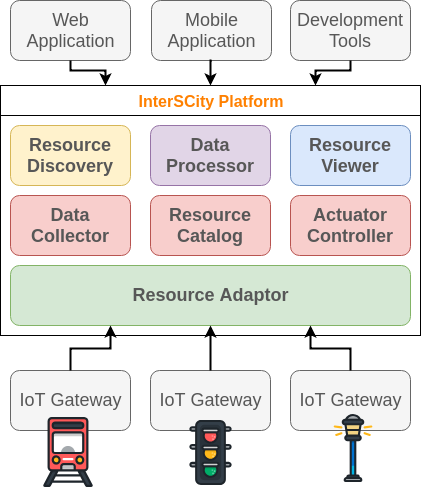
\includegraphics[width=0.5\textwidth]{figuras/platform_architecture.png}
	\caption{Arquitetura da plataforma InterSCity}
	\label{fig:platform_architecture}
\end{figure}

A comunicação entre esses microsserviços pode se dar de maneira síncrona ou assíncrona, dependendo da situação.
A comunicação síncrona é feita via API \textit{Restful}, ou seja, requisições HTTP; e a assíncrona se dá via RabbitMQ\footnote{https://www.rabbitmq.com/}, uma implementação do protocolo AMQP.
O objetivo do protocolo AMQP é criar um padrão aberto para troca de mensagens assíncronas interoperável e de larga escala~\citep{vinoski_2006}.
A principal vantagem desse protocolo é permitir que o \textit{broker} de mensagens tome as decisões de roteamento, não necessitando a aplicação ter conhecimento
desse processo~\citep{vinoski_2006}.

A plataforma traz uma abstração chamada \textit{Resource}, que representa um recurso real da cidade, como ônibus, hospital, paradas de ônibus.
Cada um desses \textit{Resources} possuem \textit{Capabilities}, que podem ser de sensoriamento ou atuação, usualmente vinculados a algum tipo de dispositivo de IoT,
como capacidade de medir temperatura ou capacidade de mudar o estado de um semáforo.
Esses conceitos são os mesmos apresentados na Seção \ref{sec:requisitos}, como requisitos para a construção de um ambiente integrado de experimentação para Cidades Inteligentes.
Como apresentado na seção anterior, semanticamente, esses recursos e capacidades aqui apresentados estarão associados a agentes e à definição de ações durante o seu
ciclo de vida no InterSCSimulator.

Nas seções a seguir, serão apresentados os dois estudos de caso envolvendo estacionamento e tráfego de carros inteligente que fizeram uso do InterSCSimulator e da plataforma InterSCity
para Cidades Inteligentes.

\section{Estacionamento Inteligente}

Neste estudo de caso, simulamos motoristas realizando seus respectivos percursos de carro e ao final procurando uma vaga disponível mais próxima ao
seu destino, provavelmente utilizando um aplicativo móvel que se comunica com a plataforma InterSCity.
Esse tipo de aplicativo poderia evitar alguns transtornos para os motoristas na árdua missão de estacionar seus carros no centro das grandes metrópoles.

A implementação deste cenário seguindo a arquitetura proposta no Capítulo \ref{cap:proposta}, bem como o experimento realizado, serão discutidos nas seções seguintes.

\subsection{Implementação}
\label{sec:smart_parking}

Ao resgatar os conceitos de recursos da cidade e capacidades para este cenário, temos os carros e as vagas de estacionamento sendo recursos, onde os carros são capazes de
fornecer a sua geolocalização (por exemplo, via GPS) e as vagas de fornecer informação quanto à sua disponibilidade (por exemplo, através de sensores infravermelhos e uma
rede de sensores).

Este cenário foi definido com o intuito de realizar experimentos envolvendo o serviço de descoberta de recursos da plataforma InterSCity.
Portanto, o aplicativo enviaria a posição do carro naquele momento, o seu destino final e o raio de busca, e a plataforma traria uma lista de vagas de estacionamento
disponíveis nas proximidades.
Já no InterSCSimulator, foi necessário realizar algumas melhorias para que os \textbf{requisitos fundamentais} fossem atendidos.
Um novo agente para gerenciar as vagas de estacionamento da cidade, chamado \textit{Parking Controller}, foi implementado.
Esse agente possui a responsabilidade de gerenciar e armazenar dados referentes às vagas de estacionamento e fazer a interface de comunicação com o componente de
integração que será apresentado mais adiante.
Além disso, modificamos o modelo de viagem do agente do tipo carro.
Anteriormente, o \textit{Carro} saia de uma origem e percorria o seu trajeto até o destino, agora, ao chegar próximo do seu destino, ele requisita uma vaga disponível mais
próxima e se dirige até ela.
Com essas melhorias, pudemos simular um cenário que se aproxima da realidade.

Para ilustrar o modelo descrito, apresentamos o ciclo de execução de um agente carro neste cenário:

\begin{enumerate}
    \item O agente \textit{Carro} é criado

    \item O caminho mais curto entre a origem e o destino é calculado

    \item O agente parte da sua origem no tempo determinado

    \item Ao chegar no nó anterior ao seu destino, uma vaga de estacionamento disponível é requisitada ao agente \textit{Parking Controller}

    \item Ao receber a vaga de estacionamento, o seu trajeto é recalculado em direção a ela

    \item O agente se direciona e estaciona na vaga descoberta 
\end{enumerate}

Um fluxo alternativo a essa execução seria o carro modificar o seu percurso em direção à vaga de estacionamento (disponível até então), e ao chegar a ela outro
carro a ter ocupado antes, sendo esse um caso comum nas grandes cidades.
Nesse caso, outra vaga de estacionamento é requisitada aumentando o seu raio de busca com o intuito de sempre encontrar vagas disponíveis.
Caso o agente do tipo carro necessitar realizar mais de três buscas de vagas disponíveis, o mesmo encerra a sua execução.

Quando o agente \textit{Carro} por fim estaciona em uma vaga disponível, o agente \textit{Parking Controller} é notificado e atualiza a sua estrutura de dados indicando
que a vaga foi ocupada pelo carro.
Esse agente é responsável também por atualizar o estado da vaga de estacionamento na plataforma.

Agora pensando nos \textbf{requisitos de integração}, o simulador precisa requisitar a plataforma em busca de vagas disponíveis mais próximas e atualizar o estado
das vagas de estacionamento.
A plataforma InterSCity provê uma API \textit{Restful} para comunicação com seus serviços (como o de descoberta de recursos), e o estado dos seus recursos podem ser
atualizados através da própria API ou via protocolo AMQP (\textit{Advanced Message Queuing Protocol}).
Esse levantamento é importante para a tomada de decisão de quais as responsabilidades e como será implementado o componente de integração.
Tendo em vista que a complexidade do componente de integração deve ser a menor possível, e a não existência de um meio de publicação de eventos em tempo de execução
no InterSCSimulator, decidimos utilizar o RabbitMQ (implementação do protocolo AMQP) na implementação desse novo meio de comunicação.
Com isso, o simulador pode atualizar o estado das vagas diretamente na plataforma de forma assíncrona, sem necessidade de auxílio do componente de integração.
As requisições HTTP feitas ao serviço de descoberta da plataforma forma realizadas pelo componente de integração, principalmente pelo fato de requisições HTTP serem
síncronas, o que poderia travar a simulação na espera por uma resposta.

Para facilitar o entendimento da integração realizada, dividiremos a explicação em duas partes: a primeira visando a requisição de vagas disponíveis mais próximas
do carro ao serviço de descoberta da plataforma InterSCity; e a segunda apresentando o fluxo de atualização do estado de uma vaga de estacionamento (ocupada
ou disponível) baseada na simulação.

A Figura \ref{fig:descoberta} apresenta a integração realizada para utilização do serviço de descoberta provido pela plataforma InterSCity.
O componente de integração foi chamado de \textit{Parking Spot Discoverer}, e foi implementado como um agente Erlang que consegue se comunicar com os agentes da
simulação via troca de mensagens.
O uso do componente de integração se fez necessário para que a simulação exerça a carga que aplicações exerceriam utilizando o protocolo HTTP para acessar
a API \textit{Restful}.
Como dito, requisições HTTP são síncronas, e sua realização dentro da simulação atrasaria consideravelmente a sua finalização, já que bloquearia a
execução dos agentes enquanto aguardariam a resposta da plataforma.
Antes de chegarmos a tal solução, implementamos uma versão onde o próprio simulador realizava requisições HTTP para a plataforma em tempo de execução, entretanto,
essa solução gerou um enorme gargalo.
Descrevemos abaixo o fluxo de atividades apresentado na Figura \ref{fig:descoberta}.

\begin{enumerate}
    \item Ao chegar a um nó, antes do seu destino, o \textit{Car} solicita a vaga de estacionamento para o agente \textit{Parking Controller}, passando a sua
	localização como parâmetro.

	\item O agente \textit{Parking Controller} envia a localização para o \textit{Parking Spot Discoverer} que solicita a vaga disponível mais próxima,
	em um raio de 500 metros.

	\item O \textit{Parking Spot Discoverer} faz uma requisição HTTP para o serviço de descoberta da plataforma que retorna a vaga em questão.
	Caso não seja encontrada uma vaga disponível (não ocupada) em um raio de 500 metros, esse raio é multiplicado por dois até que se encontre uma vaga
	disponível.

	\item O identificador da vaga é retornado para o agente \textit{Parking Controller} e ele marca a vaga como utilizada em uma estrutura de dados mantida no simulador.

    \item O identificador da vaga é recebido pelo agente \textit{Car} e a rota é recalculada para chegar até ela.
\end{enumerate}

\begin{figure}[ht]
	\centering
	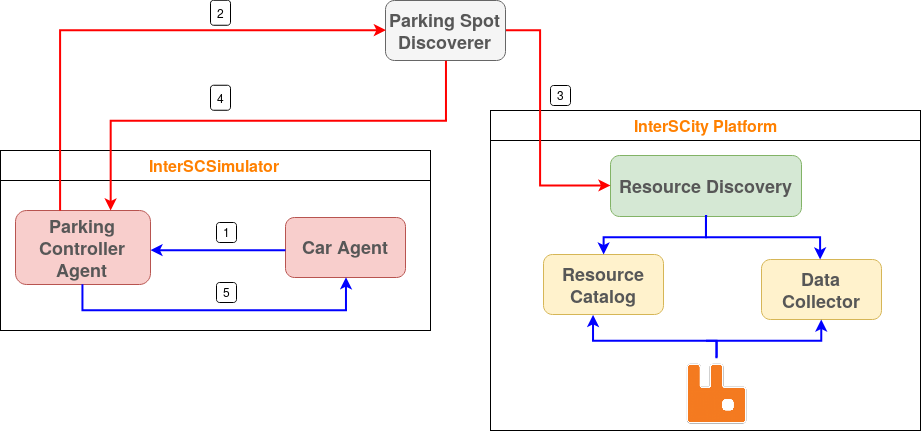
\includegraphics[width=\textwidth]{figuras/integration_get_data_smart_parking.png}
	\caption{Integração para descoberta de vagas livres próximo do destino da
	viagem}
	\label{fig:descoberta}
\end{figure}

A Figura \ref{fig:atualizacao} apresenta a integração realizada com o intuito de atualizar o estado das vagas de estacionamento na plataforma baseado nos
acontecimentos da simulação.
Como foi adicionado a funcionalidade de publicação dos eventos da simulação via RabbitMQ para os interessados, não foi necesário a utilização do
componente de integração, já que a plataforma também utiliza o mesmo protocolo para divulgação dos seus dados entre os microsserviços.
O fluxo apresentado na Figura \ref{fig:atualizacao} contém os seguintes passos.

\begin{enumerate}
    \item O agente \textit{Car} estaciona na vaga do estacionamento e notifica o \textit{Parking Controller}.

	\item O \textit{Parking Controller} informa, via \textit{RabbitMQ}, que a vaga está ocupada usando o seu identificador.

	\item O \textit{RabbitMQ} repassa esse dado para os microsserviços \textit{Resource Catalog} e \textit{Data Collector}.
\end{enumerate}

\begin{figure}[ht]
	\centering
	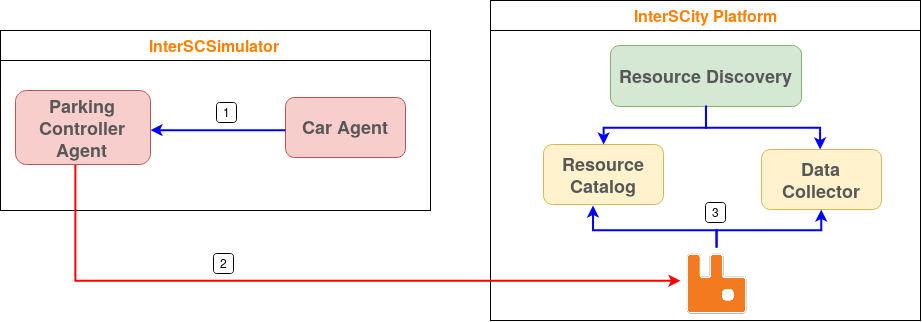
\includegraphics[width=\textwidth]{figuras/integration_publish_data_smart_parking.png}
	\caption{Integração para publicar dados}
	\label{fig:atualizacao}
\end{figure}

Vale ressaltar que as atividades 2 e 3 apresentadas na Figura \ref{fig:atualizacao} também são executadas quando a vaga é liberada.
Após dez minutos que o agente está estacionado na vaga, o agente \textit{Parking Controller} libera a vaga na estrutura de dados mantida dentro do simulador e informa o
ocorrido para a plataforma.
Com isso, a plataforma atualiza os dados da vaga quando ela é ocupada e quando liberada.

Após a implementação da arquitetura descrita, fomos capazes de executar experimentos de larga escala no contexto de estacionamento inteligente.
Os resultados obtidos serão apresentados na próxima seção.

\subsection{Experimento}
\label{sec:exp_smart_parking}

Neste experimento, tentamos verificar a escalabilidade dos microsserviços envolvidos da plataforma InterSCity, para isso utilizamos dados reais de uma das maiores metrópoles do mundo: São Paulo.
Dados abertos da cidade de São Paulo foram utilizados para a definição do cenário de simulação do ambiente integrado.
Utilizamos dados extraídos da pesquida OD (Origem-Destino) realizada pela Companhia de Metrô da cidade de São Paulo e do OpenStreet Maps para a definição de cenário.
A seguir, esses dados, bem como suas fontes, utilizados na configuração do experimento serão detalhados:

\begin{itemize}
    \item \textbf{Pesquisa Origem-Destino (OD)}: criamos as viagens de carro simuladas com base na pesquisa OD realizada pela Companhia de Metrô de São Paulo em 2007.
        \footnote{Pesquisa Origem-Destino - https://transparencia.metrosp.com.br/dataset/pesquisa-origem-e-destino/resource/dd9382bf-fbbe-4ca4-bd32-bf6150a59c4b}
        Essa pesquisa descreve as viagens de 200.000 pessoas e extrapola os dados para toda a população da cidade.
        A pesquisa inclui informações sobre a origem, o destino, o modo de transporte e a hora de partida.
        Esses dados foram utilizados para definir o comportamento dos agentes do tipo carro na simulação.
        Para gerar a carga de trabalho para a plataforma, simulamos o tráfego em São Paulo durante um dos horários de pico, das 5h40 às 8h40.
        Na pesquisa OD, há 492.976 carros que começam suas viagens durante o intervalo de tempo considerado.

    \item \textbf{OpenStreet Maps}: para criar o grafo viário da cidade de São Paulo usado na simulação, usamos o mapa do OpenStreet Maps.
        Esse mapa contém todas as ruas e junções da cidade, em conjunto com um vasto número de atributos, como comprimento, capacidade e velocidade limite.
        Tais informações são usadas pelo simulador para definir as rotas percorridas pelos carros durante a realização de suas viagens, bem como simular o impacto do tráfego na velocidade dos carros.

    \item \textbf{Vagas de Estacionamento}: criamos as vagas de estacionamento na simulação baseado nos dados obtidos através do OpenStreet Maps e do Zona Azul
        \footnote{http://www.cetsp.com.br/consultas/zona-azul/mapa-zona-azul/mapa-zona-azul.aspx}
        (serviço de estacionamento rotativo da cidade de São Paulo).
        Informações de 467.741 vagas de estacionamento foram coletadas, elas foram derivadas a partir de dados de estacionamentos obtidos através do OpenStreet Maps, onde é possível obter
        a capacidade máxima (número de carros), e de vagas individuais do Zona Azul.
\end{itemize}

Nas Figuras \ref{fig:map-spots-distribution} e \ref{fig:map-destinations-distribution}, são apresentadas as distribuições das vagas de estacionamento e destinos de viagens de carros, respectivamente,
utilizadas nesse experimento.
Os destinos apresentados na Figura \ref{fig:map-destinations-distribution}, são referentes a todas as viagens realizadas no decorrer de toda a simulação.
É importante notar que a distribuição das vagas de estacionamento baseada nesses dados reais está mais concentrada no centro da cidade do que os destinos das viagens.
Isso pode levar a situaçãoes onde o agente do tipo carro pode realizar mais de três tentativas de busca de vagas disponíveis e ainda sim não conseguir estacionar.
Nesse caso, o usuário do aplicativo pararia de utilizá-lo e o agente do tipo carro terminaria sua execução, como apresentado na Seção \ref{sec:smart_parking}.

\begin{figure}[!ht]
    \centering
    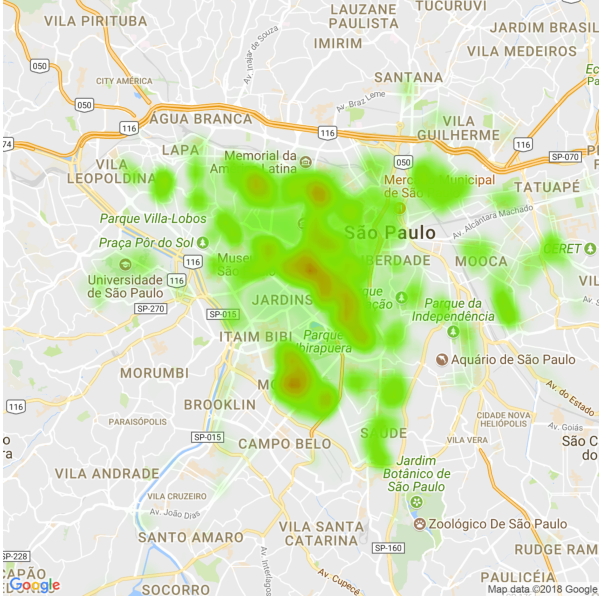
\includegraphics[width=8cm]{figuras/mapa_vagas.pdf}
    \caption{Mapa de calor com a distribuição das vagas de estacionamento utilizadas no experimento.}
    \label{fig:map-spots-distribution}
\end{figure}

\begin{figure}[!ht]
    \centering
    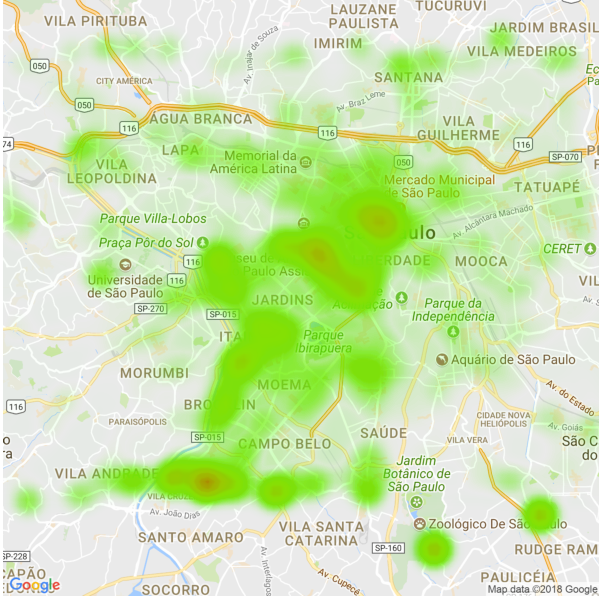
\includegraphics[width=8cm]{figuras/mapa_viagens.pdf}
    \caption{Mapa de calor com a distribuição dos destinos de viagens de carro utilizadas no experimento.}
    \label{fig:map-destinations-distribution}
\end{figure}

Os passos a seguir foram executados no decorrer desse experimento:

\begin{enumerate}
    \item Execução de uma instância em modo de produção da plataforma InterSCity em um ambiente de nuvem. Esse ambiente proporciona maior flexibilidade para variação do número de microsserviços em tempo
        de execução.

    \item Habilitação do mecanismo de elasticidade automática (\textit{auto-scaling}) para os microsserviços da plataforma baseado na variação de carga de trabalho.

    \item Configuração do simulador em um ambiente isolado da plataforma. Assim, o gasto de recursos computacionais do simulador não interfere no uso da plataforma.

    \item Realização da simulação do cenário de estacionamento inteligente.

    \item Monitoramento do desempenho e o uso de recursos da plataforma durante toda a simulação.

    \item Analize os resultados obtidos.
\end{enumerate}

Inicialmente, foi necessária a configuração de ambas as ferramentas em conjunto com seu componente de integração em um ambiente de nuvem.
Os microsserviços da plataforma InterSCity, o simulador InterSCSimulator e ferramentas auxiliares foram implantados na forma de contêineres Docker \footnote{https://www.docker.com/}.
Utilizamos a infraestrutura provida pelo Google Cloud Platform (GCP) \footnote{https://cloud.google.com/} para a realização do experimento, sendo esse o ambiente ideal para a execução da plataforma
InteSCity, como visto na Seção \ref{sec:interscity}.
No contexto do GCP, fizemos bastante uso do Google Kubernetes Engine (GKE), sendo esse um serviço que provê um ambiente gerenciado e de produção para implantação de contêineres de
aplicações.
O Kubernetes foi utilizado principalemte para automatizar a reinicialização, a replicação e dimensionamento do número de contêineres.
Além disso, o kubernetes traz uma vantagem para a reprodutibilidade do experimento que é a especificação da infraestrutura como código, garantindo a correta aplicação das regras de implantação.
Todo o código fonte utilizado para a realização desse experimento está disponível como software livre na web \footnote{https://github.com/LSS-USP/interscity-k8s-experiment}.

Nós dividimos o \textit{cluster} utilizado em cinco diferentes \textit{pools} de máquinas virtuais para que o Kubernetes pudesse gerenciar os contêineres no contexto apropriado.
Na Figura \ref{fig:node-pools}, são apresentados os \textit{pools} de nós, contendo o número e o tipo de máquinas virtuais utilizadas por cada um no GCP
\footnote{https://cloud.google.com/compute/docs/machine-types}.
O \textit{pool} da plataforma possui 25 máquinas do tipo n1-standard-2 (2 CPUs virtuais e 7.5GB memória) e executa os microsserviços da plataforma InterSCity.
Existem três conjuntos de nós adicionais (representados em azul) compostos por n1-high-2 máquinas (2 CPUs virtuais e 13GB de memória), que executam os serviços de suporte da plataforma InterSCity.
Ambos MongoDB e PostgreSQL têm 5 nós sendo executados de maneira distribuída, instâncias tolerantes a falha de seus respectivos sistemas de banco de dados.
O RabbitMQ possui uma máquina dedicada em um \textit{pool} isolado.
MongoDB é implementado usando a estratégia de conjunto de réplicas (\textit{replica set}), onde operações de leitura são distribuídas entre nós secundários (escravos), e operações de escrita são
sempre executadas no nó primário (mestre).
A mesma estratégia é adotada na implantação do PostgreSQL, para otimizar as operações de leitura executadas pelo \textit{Resource Catalog}.
Finalmente, o InterSCSimulator é executado em sua própria máquina n1-highmem-16 (16 CPUs virtuais e 104 GB de memória), isoladas do resto do serviços.

\begin{figure}[ht]
	\centering
	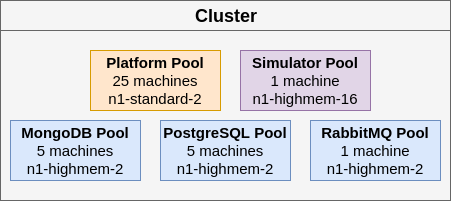
\includegraphics[width=0.7\textwidth]{figuras/node-pools.png}
    \caption{Configuração do \textit{cluster} para o experimento.}
	\label{fig:node-pools}
\end{figure}


Para o conjunto de nós da plataforma, o Kubernetes pode programar a implantação de vários contêineres para a mesma máquina, dependendo da disponibilidade de recursos computacionais.
A distribuição de contêineres nos 25 nós pode diferir de uma rodada do experimento para a outra, e é uma variável que não controlamos durante o experimento.
Para avaliar o impacto de tais variações na análise, realizamos 15 rodadas desse experimento e verificamos a variabilidade dos resultados.

Como estávamos interessados em avaliar a escalabilidade da plataforma considerando um cenário de Cidades Inteligentes com uma carga de trabalho variável, usamos dimensionamento automático
(\textit{auto-scaling}) para o \textit{Resource Catalog}, \textit{Resource Discovery}, \textit{Data Collector}, já que eles são projetados para escalar horizontalmente.
Para esse propósito, especificamos um valor alvo de 60\% de uso da CPU para cada um desses serviços, permitindo que o sistema aumente ou diminua o número de contêineres por serviço baseado nisso.
O sistema balanceia a carga de trabalho para corresponder ao valor alvo de uso da CPU, considerando o uso médio da CPU dos contêineres em execução, que é medido a cada 30 segundos.
Inicialmente, cada serviço tem quatro contêineres, que é definido como o número mínimo de contêineres em execução.
Esse número pode aumentar à medida que os recursos computacionais ficarem disponíveis no \textit{pool} de nós da plataforma.
Os contêineres são executados por trás de um serviço de balanceamento de carga.

Embora possamos nos beneficiar das propriedades de elasticidade do GCP, adicionando e removendo automaticamente nós ao \textit{cluster} através da sua funcionalidade de dimensionamento automático,
isso introduziria outro nível de incerteza em nosso experimento, já que, na nossa experiência, o tempo levado para criar novas máquinas virtuais pode variar consideravelmente.
Sabendo disso, criamos todos os nós previamente, antes de iniciar o experimento, mantendo-os em execução ao longo de todo experimento.

Como dito anteriormente, executamos 15 rodadas de experimentos, onde cada uma durou 3h, correspondendo ao horário de pico da manhã da cidade de São Paulo descrito no início desta seção.
Na Figura \ref{fig:workload}, podemos ver a carga de trabalho média gerada pela simulação durante todo o experimento e o seu desvio padrão (linhas pretas no topo de cada barra).
Vale notar que nos primeiros 80 minutos de simulação, temos um crescimento constante da carga de trabalho.
No intervalo aproximado de uma hora, entre 60 e 120 minutos, observamos o período de maior carga do experimento, considerando que o pico máximo de requisições ocorre após 80 minutos, correspondendo a mais
de 113.000 requisições em 10 minutos.
No total, mais de um milhão de requisições foram realizadas para a plataforma durante o tempo de experimento.
Considerando que para responder cada uma dessas requisições requer um conjunto complexo de operações com várias etapas internas, isso se traduz em uma carga computacional muito alta.

\begin{figure}[ht]
	\centering
	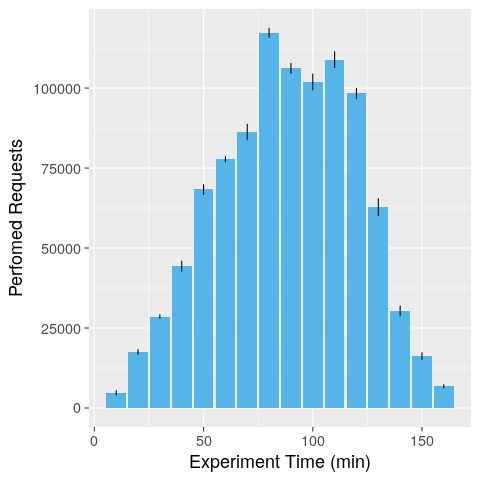
\includegraphics[width=0.7\textwidth]{figuras/workload.png}
    \caption{Média da carga de trabalho gerada pelo InterSCSimulator no decorrer do experimento.}
	\label{fig:workload}
\end{figure}

A Figura \ref{fig:auto-scaling} mostra a criação e destruição dinâmica de contêineres da plataforma InterSCity devido à aplicação da estratégia de dimensionamento automático em uma única rodada
do experimento.
A replicação inicial das instâncias de Kong (balaceador de carga) foi suficiente para suportar toda a carga de trabalho durante todo o experimento, já que ele executa apenas a tarefa leve
de encaminhar as requisições de entrada aos microsserviços apropriados.
Por sua vez, os três microsserviços da plataforma, que são responsáveis por processar as requisições de fato, foram replicados de acordo com o aumento da carga de trabalho.
Portanto, o número de contêineres para cada um desses serviços variou de 4 a 25.
É importante mencionar que o mecanismo de elasticidade da plataforma InterSCity também reduziu o número de contêineres à medida que a demanda diminuiu.
Como pode ser visto na Figura \ref{fig:auto-scaling}, dentre os microsserviços da plataforma, o \textit{Data Collector} foi o microsserviço que consumiu menos tempo de CPU.

\begin{figure}[ht]
	\centering
	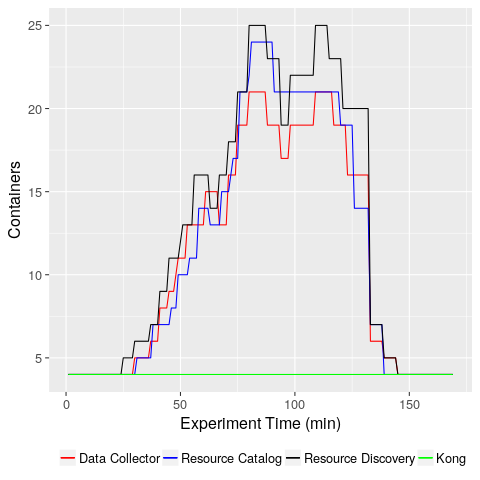
\includegraphics[width=0.7\textwidth]{figuras/auto-scaling.png}
    \caption{Dimensionamento automáticos dos microsserviços da plataforma InterSCity.}
	\label{fig:auto-scaling}
\end{figure}


A Figura \ref{fig:throughput} mostra a taxa de vazão (\textit{throughput}) média da plataforma InterSCity ao longo da duração do experimento.
A taxa de vazão é definida como a taxa de respostas bem sucedidas recebidas pelo componente de integração.
O resultado indica que a taxa de vazão corresponde de perto a carga de trabalho gerada, como pode ser visto comparando as Figuras \ref{fig:workload} e \ref{fig:throughput}.
A plataforma foi capaz de lidar com a demanda variável graças à sua escalabilidade e funcionalidade de dimensionamento automático, descritos na Seção \ref{sec:interscity}.
No entanto, devemos mencionar que a taxa de vazão não correspondeu exatamente à carga de trabalho gerada, pois algumas requisições falharam, representando em média quase 0,6\% de todas as requisições.
As requisições com falha incluem aquelas que tiveram respostas com um código de erro HTTP, bem como aquelas que não foram concluídos devido a recusa de conexão ou \textit{timeout}.
Todavia, consideramos que, ser capaz de lidar com, em média, mais de 99,4\% das requisições sob alta carga é satisfatório; um usuário típico perceberia uma falha a cada 200 requisições, o que é muito bom para
este tipo de aplicação de Cidades Inteligentes em tempo real.

\begin{figure}[ht]
	\centering
	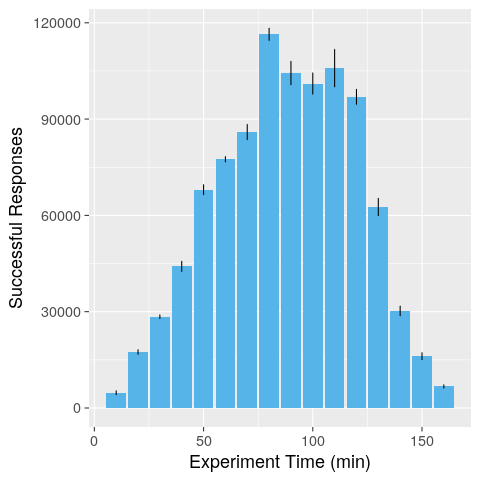
\includegraphics[width=0.7\textwidth]{figuras/throughput.png}
    \caption{Taxa de vazão (\textit{throughput}) média da platafora InterSCity.}
	\label{fig:throughput}
\end{figure}


Outro aspecto fundamental da avaliação de um sistema é analisar o desempenho da plataforma para lidar com requisições de aplicações com uma carga de trabalho variável.
A esse respeito, estamos interessados principalmente em analisar a degradação do desempenho e verificar se a plataforma está sendo dimensionada adequadamente para atender seus clientes dentro de tempos
de resposta aceitáveis.
Para tanto, coletamos o tempo de resposta do ponto de vista do cliente, como mostrado Figura \ref{fig:responsetime}.
Durante a maior parte do experimento, a plataforma foi capaz de responder em menos de um segundo.
No entanto, diferente da taxa de vazão, o impacto do maior período de demanda no tempo de resposta observado é perceptível, uma vez que, durante um intervalo curto (após 110 minutos de execução),
o tempo médio de resposta foi maior que 1 segundo.
O tempo de resposta voltou para 500 milisegundos depois disso.
Entretanto, podemos ver que, mesmo em períodos de alta carga, o tempo de resposta foi mantido abaixo de 2 segundos, o que é um resultado muito bom para esse tipo de aplicação.

\begin{figure}[ht]
	\centering
	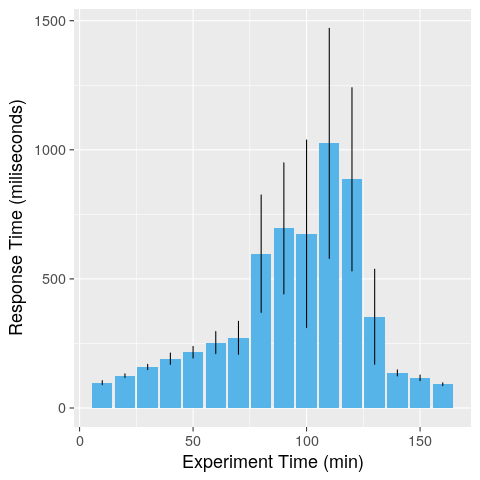
\includegraphics[width=0.7\textwidth]{figuras/response_time_mean.png}
    \caption{Tempo de resposta médio da platafora InterSCity.}
	\label{fig:responsetime}
\end{figure}


Devemos ter em mente que a distribuição de contêineres nos nós disponíveis podem impactar o tempo de resposta, pois vários contêineres podem competir por recursos computacionais se estiverem
sendo executados na mesma máquina.
Além disso, embora o sistema realize a tarefa de dimensionamento automático a cada 30 segundos, não temos controle sobre o tempo que leva para um \textit{container} ser criado, implantado e ficar pronto
para receber novas requisições.
Por outro lado, essa distribuição também pode introduzir um efeito benéfico devido à possível implantação de serviços que constantemente interagem uns com os outros na mesma máquina, reduzindo a latência
de rede e imprevisibilidade.

Ao final desse estudo de caso, percebemos que não exercitamos todos os requisitos apresentados para a construção de um ambiente simulado e integrado para experimentação de plataformas de Cidades Inteligentes.
Por isso, realizamos um segundo estudo de caso, onde a \textbf{atuação} no ambiente simulado se fez necessária, apresentado na seção seguinte.

\section{Tráfego de Carros Inteligente}

Com o objetivo de exercitar o envio de comandos de atuação da plataforma para o ambiente simulado, que não foi explorado no cenário de estacionamento inteligente, definimos um novo cenário.
Neste caso, visamos identificar trechos em vias da cidade com tráfego de carros anômalo (devido ao fechamento de ruas, acidentes, desastres naturais e etc.) e notificar
previamente os motoristas para evitarem passar naquele trecho através de Placas de Mensagens Variadas (PMVs).
Veja na Figura \ref{fig:pmv} uma PMV.
Consideramos aqui uma anomalia uma variação considerável na velocidade média dos carros que trafegam naquele trecho de via naquele horário.
Essas PMVs são posicionadas em pontos estratégicos da cidade e apresentam alertas aos motoristas em tempo real sobre possíveis anomalias no trânsito.
E, com isso, motoristas podem mudar o seu percurso evitando maiores congestionamentos na cidade.

\begin{figure}[ht]
	\centering
	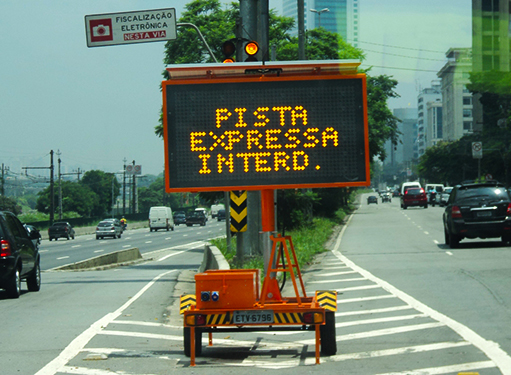
\includegraphics[width=0.7\textwidth]{figuras/pmv.jpg}
    \caption{Exemplo de Placa de Mensagem Variada.}
	\label{fig:pmv}
\end{figure}


A implementação deste cenário seguindo a arquitetura proposta no Capítulo \ref{cap:proposta}, bem como o experimento realizado, serão discutidos nas seções seguintes.

\subsection{Implementação}
\label{sec:smart_traffic}

Essencialmente, o cenário de tráfego de carros inteligente funciona da seguinte forma:

\begin{enumerate}
    \item A plataforma coleta dados históricos de posicionamento dos carros em seus trajetos, a partir desses pontos a velocidade média dos carros é calculada e o método MAD (\textit{Median Absolute Deviation}
        - Desvio Absoluto da Mediana)\citep{leys_2013} é utilizado para definir limiares (\textit{thresholds}) de velocidade média para cada trecho de via da cidade em cada horário, sendo esses limiares
        valores de velocidade média aceitáveis em um dia comum.
        Para isso, o ambiente simulado envia dados de posicionamento georreferenciado dos carros a cada ciclo de execução, simulando por exemplo um dispositivo que contém um
        sistema de GPRS (\textit{General Packet Radio Service}) + GPS (\textit{Global Positioning System}).
        Com uma série de pontos de onde o carro passou em cada instante, se torna possível calcular a sua velocidade média, logo obtemos a velocidade média de carros
        que passaram naquele trecho naquele dado momento durante todo o dia.
        Tendo esses limiares calculados usando o MAD, a plataforma se torna capaz de identificar anomalias na velocidade média dos carros em tempo real, verificando se a variação naquele instante
        extrapola ou não o que foi identificado com os dados históricos.

    \item Ao identifiar uma anomalia de trânsito em algum trecho, a plataforma identifica as PMVs mais próximas do incidente e atualiza a sua mensagem informando os motoristas
        do ocorrido.

    \item Caso o motorista passe por uma PMV contendo essa mensagem, ele verifica se o trecho mencionado faz parte do seu percurso. Sendo verdade, ele recalcula a sua
        rota evitando maiores congestionamentos na região.
\end{enumerate}

Nesse cenário de experimentação, o novo serviço de processamento de dados (históricos e de tempo real), que está em desenvolvimento, e o envio de comandos de atuação da plataforma
InterSCity puderam também ser testados.
Além disso, foi possível finalizar a validação da arquitetura proposta para a criação de um ambiente para experimentação em plataformas de Cidades Inteligentes,
implementando a atuação em tempo real no ambiente simulado.

Para realizar experimentos envolvendo essas funcionalidades da plataforma InterSCity, foi necessário implementar o conceito de PMVs, eventos de fechamentos de via e de
processamento de comandos de atuação em tempo de execuação no InterSCSimulator.
Foi utilizada a publicação de eventos (dados de sensores) implementado para o cenário anterior, já que para o funcionamento do serviço de processamento de dados
em tempo real da plataforma precisamos enviar a cada ciclo de execução da simulação o posicionamento de todos os carros presentes.
Essas funcionalidades são essenciais para atender os \textbf{requisitos fundamentais} para esse cenário.

O modo de publicação de dados em tempo de execução no InterSCSimulator foi refatorado para melhor atender ambos os cenários implementados.
Como visto no cenário anterior, a publicação de eventos da simulação se dava através do agente \textit{Parking Controller} (como pode ser visto na Figura \ref{fig:atualizacao}), já que
até então o único tipo de evento publicado pelo simulador era a atualização da disponibilidade de uma vaga de estacionamento.
No intuito de permitir que outros agentes da simulação também pudessem publicar os seus eventos, um novo agente chamado \textit{Publisher} foi criado, removendo essa responsabilidade
anteriormente atribuída ao agente \textit{Parking Controller}.
%Desse modo, o agente do tipo carro também se tornou capaz de publicar a sua posição, onde a cada ciclo de execução é enviada uma mensagem a um agente \textit{Publisher} contendo sua localização.
Agora, qualquer agente da simulação que deseje publicar um evento deve apenas enviar uma mensagem ao \textit{Publisher} com o conteúdo do evento.
Desse modo, o agente do tipo carro envia a cada ciclo de execução uma mensagem a um agente \textit{Publisher} contendo sua localização, tornando-se capaz de pulicar a sua posição.

Visando tornar factível a simulação de eventos de fechamento de vias na cidade, adicionamos o conceito de eventos de trânsito ao InterSCSimulator.
Um novo arquivo de entrada para o simulador e um novo agente foram adicionados.
O novo arquivo de entrada (chamado por padrão \textit{events.xml}), contem uma lista de eventos de fechamento de via que serão agendados na simulação.
Como pode ser visto na Listagem \ref{code:events}, cada evento é representado por uma lista de atributos separados por ponto e vírgula ('';``), e os atributos são os seguintes:
(i) o tipo do evento de trânsito (\textit{close\_street} para fechamento de vias e \textit{reduce\_capacity} para redução da capacidade de vias);
(ii) o número identificador da via a ser fechada (aresta no grafo da cidade);
(iii) o número do ciclo de simulação onde deve ser iniciado o evento;
(iv) o número de ciclos de simulação que deve durar o evento;
(v) a porcentagem da capacidade do fluxo de carros que ainda estará em funcionamento, usada no caso de um fechamento parcial do trecho (se o evento for de fechamento de via deve-se utilizar o valor 0).
O novo agente chamado \textit{Events Manager} é responsável por agendar todos esses eventos no início da simulação e alterar o grafo da cidade no momento programado.
Quando o trecho da via é fechado, a aresta do grafo da cidade é removida momentaneamnte até o evento ser encerrado, impedindo assim a possibilidade de passagem de qualquer
carro.
Quando o evento apenas reduz a capacidade de fluxo de carros da via, modificamos a sua capacidade para atender o que foi programado até o evento ser encerrado.
Essa capacidade é um atributo dado àquela aresta do grafo.

\lstset{
    language=xml,
    tabsize=3,
    frame=lines,
    caption=Arquivo de entrada contendo os eventos de fechamento de vias,
    label=code:events,
    frame=shadowbox,
    rulesepcolor=\color{gray},
    xleftmargin=20pt,
    framexleftmargin=15pt,
    keywordstyle=\color{blue}\bf,
    commentstyle=\color{OliveGreen},
    stringstyle=\color{red},
    numbers=left,
    numberstyle=\tiny,
    numbersep=5pt,
    breaklines=true,
    showstringspaces=false,
    basicstyle=\footnotesize,
    emph={uuid,node},emphstyle={\color{magenta}}}
    \lstinputlisting{files/events.csv}

Para a representação das PMVs no InterSCSimulator, foi criado um agente chamado \textit{PMV Manager}.
Seu papel é atualizar as mensagens de PMVs.
As PMVs em si foram implementadas como atributos de vértices do grafo da cidade (sendo os vértices o encontro de duas ou mais vias).
Nesse atributo, é guardada uma lista de trechos de vias (arestas) onde foram encontradas alguma anomalia no trânsito.
Os agentes do tipo carro, ao passar por um vértice que contém esse atributo, verificam se alguma das arestas ali presentes fazem parte do seu trajeto ou não.
Caso positivo, o seu percurso é recalculado.
Caso contrário, ele se mantém inalterado.

A última implementação no InterSCSimulator necessária para atender os requisitos apresentados seguindo a arquitetura proposta foi o recebimento de comandos de atuação e
seu processamento em tempo de execução.
Essa funcionalidade é fundamental para a atualização das PMVs em tempo de execução pela plataforma.
Diante disso, mais um novo agente foi criado para ficar à espera desses comandos enviados pela plataforma: o \textit{Listener}.
Como um comando de atuação pode ser enviado a qualquer momento, foi necessário criar esse novo agente, cuja única responsabilidade é receber esse comando e armazená-lo em uma
estrutura de dados, para que outros agentes não ficassem bloqueados (bloqueando também a simulação) a espera de tal acontecimento.
Ou seja, esse agente fica em um laço (\textit{loop}) infinito a espera de uma mensagem que é enviada via AMQP (mesmo protocolo utilizado para publicação dos dados).
%A utilização do RabbitMQ foi escolhida devido a possibilidade da plataforma InterSCity enviar comandos de atuação através do mesmo, e como foi uma funcionalidade nova,
%decidimos utilizar a mesma tecnologia, reduzindo assim o problema de interoperabilidade.
Por essa ser uma nova funcionalidade, decidimos utilizar o mesmo protocolo e a mesma tecnologia utilizada pela plataforma InterSCity visando reduzir o problema de interoperabilidade.
O RabbitMQ, que já vinha sendo utilizado pela plataforma para envio de comandos de atuação, foi selecionado como ferramenta para tratamento de eventos da simulação, tanto para publicação quanto para 
recebimento.
Quando um comando é recebido, no caso uma aresta de trecho anômalo a ser atualizada em uma PMV, o \textit{Listener} armazena essa mensagem em uma estrutura de dados que é acessada no
próximo ciclo de execução pelo \textit{PMV Manager} que, por sua vez, atualiza o atributo da referida PMV (vértice no grafo).

Após a apresentação das funcionalidades e melhorias implementadas, as duas vias de fluxo de comunicação entre o simulador e a plataforma serão apresentadas a seguir.
Na Figura \ref{fig:smart_traffic_publish_data}, os passos para a publicação dos dados de posicionamento de cada um dos carros a cada ciclo de execução são expostos.

\begin{figure}[ht]
	\centering
	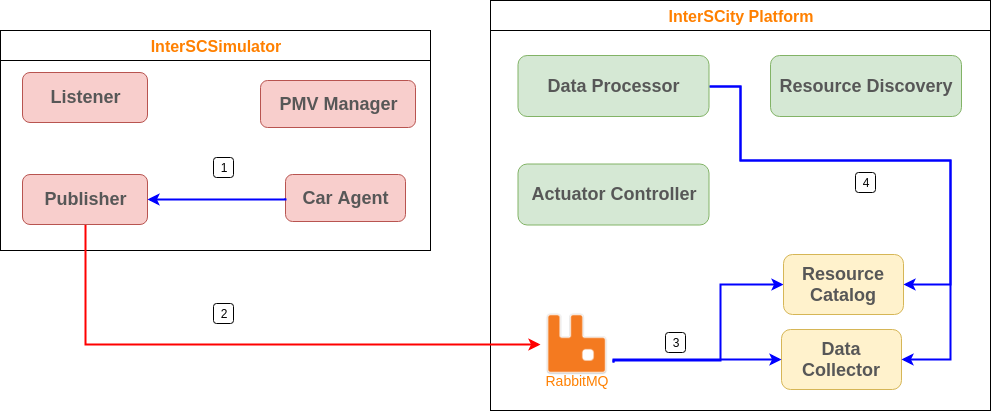
\includegraphics[width=\textwidth]{figuras/integration-publish-car-position.png}
	\caption{Integração para publicar dados de posicionameto de carros}
	\label{fig:smart_traffic_publish_data}
\end{figure}

\begin{enumerate}
    \item O agente do tipo carro a cada ciclo de execução envia uma mensagem para o agente \textit{Publisher} contendo a sua posição naquele dado momento.

    \item O agente \textit{Publisher} se conecta ao \textit{broker} do RabbitMQ e publica uma mensagem contendo: o identificador do carro, o seu posicionamento e o \textit{timestamp}.

    \item Os microsserviços \textit{Resource Catalog} e \textit{Data Collector} são notificados e recebem tais dados. O \textit{Resource Catalog} atualiza o último dado monitorado
        daquele carro, e o \textit{Data Collector} atualiza a sua base de dados contendo todas as medições.

    \item O microsserviço \textit{Data Processor} acessa dados armazenados por esses outros serviços com o intuito de definir limiares para velocidade média de vias (dados históricos),
        ou para identificar anomalias no trânsito (fluxo de dados em tempo real).
\end{enumerate}

Já na Figura \ref{fig:smart_traffic_actuation}, é apresentado o fluxo para atualização da lista de trechos anômalos de vias em PMVs, representando aqui um comando de atuação no
ambiente simulado.
Lembrando que o gatilho para a execução desse processo é o serviço de processamento de dados identificar alguma anomalia no trânsito.

\begin{figure}[ht]
	\centering
	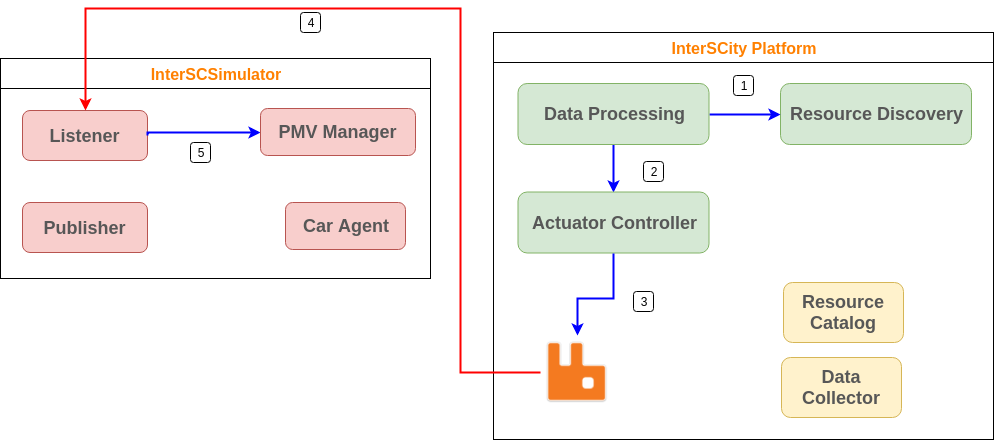
\includegraphics[width=\textwidth]{figuras/integration-actuate-pmv.png}
	\caption{Integração para atuação em Placas de Mensagens Variadas}
	\label{fig:smart_traffic_actuation}
\end{figure}

\begin{enumerate}
    \item O \textit{Data Processor}, ao identificar uma anomalia no trânsito em determinado ponto da cidade, requisita ao \textit{Resource Discovery} as PMVs mais próximas
        daquele ponto, para que elas possam ser atualizadas.

    \item Ao serem identificados as PMVs, o \textit{Data Processor} envia os identificadores das PMVs e do trecho anômalo para o \textit{Actuator Controller}.

    \item O \textit{Actuator Controller} formata essas mensagens e as publica em um dos canais do RabbitMQ.

    \item O agente \textit{Listener}, cujo único papel é esperar por esse tipo de mensagem, a recebe e a armazena em uma estrutura de dados compartilhada pelos agentes do simulador.

    \item O agente \textit{PMV Manager} verifica a presença dessa nova mensagem na estrutura de dados compatilhada, e atualiza o atributo que representa a PMV no vértice do grafo
        viário da cidade, adicionando mais esse trecho para a lista presente ou criando-a caso não exista nenhum outro trecho.
\end{enumerate}

Um ponto interessante desse segundo cenário, foi a não necessidade de um componente de integração, já que ambas as ferramentas se comunicam através do mesmo protocolo (inclusive a
mesma ferramenta) e conseguem representar os mesmos conceitos de maneira equivalente.
Esse é o cenário ideal para criação de um ambiente simulado de experimentação para uma plataforma de Cidades Inteligentes, já que não foi essencial a implementação desse
componente extra que, como discutido, traria mais complexidade para o sistema, podendo aumentar o tempo de resposta entra as ferramentas.
Claro que tudo isso foi possível porque neste mesmo trabalho fizemos toda a implementação dos \textbf{requisitos fundamentais} apresentados, portanto,
tivemos a oportunidade de tomar as decisões técnicas que facilitaram a integração entre as duas ferramentas.


\subsection{Experimento}

Esse experimento consistiu em três cenários.
Conforme descrito na Seção \ref{sec:smart_traffic}, limiares (\textit{thresholds}) de velocidade média para cada trecho de via em cada horário do dia deveriam ser definidos.
Portanto, o primeiro cenário consistiu na simulação do trânsito da cidade sem nenhum evento de fechamento de via, ou seja, o trânsito normal da cidade.
Para tanto, a aplicação de detecção de anomalias foi capaz de, com os dados de posicionamento de carros enviados a cada ciclo de execução, definir esses tais limiares através do método MAD.
O segundo cenário, consistiu em simular o trânsito de carros na cidade com alguns eventos de fechamento de vias (representando ruas alagadas, acidentes de carro, etc.).
Nesse cenário, simulamos o comportamento caótico visto nas grandes cidades, onde vias são interditadas e interferem diretamente no tráfego dos carros.
No último cenário, simulamos o mesmo comportamento do segundo cenário, mas adicionamos as PMVs para auxiliar os condutores de carros a contornar tais situações.
Tendo em vista que os limiares já haviam sido definidos, a aplicação, sem ter conhecimento prévio dessas vias fechadas, detectava automaticamente esses trechos e notificava os motoristas através da
atualização de mensagens nas PMVs.
O objetivo desses três cenários era verificar o impacto do uso de PMVs no tempo de duração médio das viagens de carro em situações de incidentes que inviabilizam a utilização de certas vias em uma cidade.

Para verificar o bom funcionamento desse cenário no ambiente simulado, dividimos esse experimento em dois.
Na primeira parte, realizamos um experimento numa escala menor e com dados fictícios, visando meramente a validação do comportamento esperado e interação entre os componentes.
Na segunda parte, utilizamos dados abertos da cidade de São Paulo, aumentando a escala do experimento e se aproximando de um cenário mais realista.
O código fonte para a execução do experimento e a análise apresentada, nesta seção, estão disponíveis em nosso repositório aberto
\footnote{https://github.com/LSS-USP/pmv\_experiment/blob/master/Analysis.ipynb}.

\subsubsection{Validação}

Nesse experimento inicial de validação, os três cenários com o que diz respeito ao número de eventos de fechamento de via e PMVs, se deram da seguinte forma:

\begin{enumerate}
    \item Sem eventos de fechamento de via e sem PMVs

    \item Com um evento de fechamento de via e sem PMVs

    \item Com um evento de fechamento de via e uma PMV
\end{enumerate}

Foram executadas 20 iterações de cada uma dos cenários, onde em cada iteração corresponde a 10 minutos de simulação.
Em todos os cenários, utilizamos um grafo com 8 vértices e 16 arestas, como pode ser visto na Figura \ref{fig:mapa_validacao}.
O grafo é direcionado, onde cada aresta na verdade representa duas, sendo uma entrando e outra saíndo de seus vértices, ou seja, simbolizam vias de mão dupla.

\begin{figure}[ht]
	\centering
	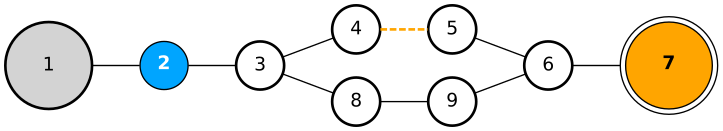
\includegraphics[width=\textwidth]{figuras/mapa_validacao.png}
	\caption{Mapa viário da cidade utilizado para validação.}
	\label{fig:mapa_validacao}
\end{figure}

O grafo da Figura \ref{fig:mapa_validacao} retrata o mapa viário da cidade simulada da seguinte forma:

\begin{itemize}
    \item Os vértices representam início e/ou fim de uma ou mais ruas.

    \item As arestas representam segmentos de vias da cidade.

    \item Todas as arestas possuem comprimento 1. Por isso, a cada ciclo de simulação, caso seja possível, um carro percorre uma aresta.
\end{itemize}

Além disso, adotamos a seguinte forma para separar vértices e arestas que desempenham papel importante neste experimento:

\begin{itemize}
    \item A aresta pontilhada amarela representa a via da cidade que será fechada durante a simulação (essa aresta só será afetada nos cenários que posssuem tal evento).

    \item O vértice 1 (em cinza) representa a origem de todas as viagens simuladas.

    \item O vértice 7 (em alaranjado) representa o destino das viagens.

    \item O vértice 2 (em azul) representa o local da cidade que contém uma PMV que alertará os motoristas sobre possíveis anomalias nas vias.
\end{itemize}

Em todas as iterações de todos os cenários, simulamos um total de 100 carros realizando viagens partindo do vértice 1 até o 7, onde metade dos carros partem no início da simulação e o restante após 50 ciclos
de execução.
Como o intuito desse experimento era validar o comportamento da implementação do ambiente de experimentação como um todo, antes de apresentar os resultados obtidos, descrevemos o resultado esperado para
cada um dos cenários a seguir.

Na Figura \ref{fig:mapa_etapa1}, pode-se ver o caminho esperado que os carros percorrecem no primeiro cenário do experimento, onde não há a presença de eventos de fechamento de vias, e muito menos PMV.
As arestas em \textbf{roxo} representam o trajeto do carro, as demais arestas não utilizadas foram removidas do grafo a título de legibilidade.
Note que ao chegar no vértice 3, ele sempre optará o caminho seguindo pelo vértice 4.
Isso acontece porque todas as arestas possuem o mesmo comprimento (ambos são um caminho mais curto até o destino), sendo critério de desempate o menor índice.

\begin{figure}[ht]
	\centering
	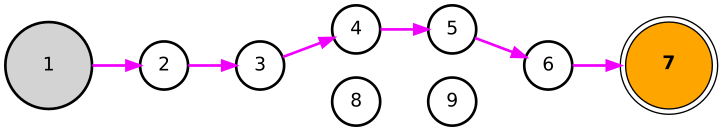
\includegraphics[width=\textwidth]{figuras/mapa_etapa1.png}
	\caption{Trajeto esperado do cenário 1 do experimento.}
	\label{fig:mapa_etapa1}
\end{figure}

Na Figura \ref{fig:mapa_etapa2}, o trajeto esperado para que o carro percorra no cenário 2 do experimento é apresentado.
Nesse cenário, temos uma via fechada, sendo ela entre os vétices 4 e 5, e nenhuma PMV para auxiliar os motoristas.
Em \textbf{roxo} podemos ver as arestas que serão percorridas inicialmente;
em cor \textbf{preta}, as arestas que faziam parte do caminho inicialmente calculado, mas que não foram percorridas devido ao fechamento da via (aresta tracejada);
e em cor \textbf{verde}, o caminho recalculado após se deparar com o fechamento de via no vértice 4.

\begin{figure}[ht]
	\centering
	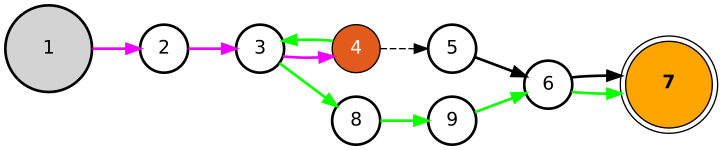
\includegraphics[width=\textwidth]{figuras/mapa_etapa2.png}
	\caption{Trajeto esperado do cenário 2 do experimento.}
	\label{fig:mapa_etapa2}
\end{figure}

Por fim, na Figura \ref{fig:mapa_etapa3}, temos a dinâmica esperada para o cenário 3, onde existe o fechamento da via. Contudo, a PMV se faz presente para notificar os condutores de veículos.
Mais uma vez, a via representada pela aresta 4 -> 5 é fechada, e a PMV é posicionada no vértice 2 representado em azul.
Utilizamos aqui a mesma notação anterior.
A aresta \textbf{roxa} representa o caminho inicialmente calculado e que foi percorrido;
as arestas \textbf{pretas} faziam parte do caminho inicial, mas nesse caso não foram percorridas devido ao fechamento da via e da PMV;
e as \textbf{verdes} simbolizam o novo caminho recalculado após o motorista ter sido notificado pela PMV.
No modelo implementado, ainda assim, era esperado que alguns carros percorresem o fluxo apresentado na Figura \ref{fig:mapa_etapa2}, já que acreditamos que nem todos os motoristas que vissem
a notificação iriam de fato mudar o seu trajeto.

\begin{figure}[ht]
	\centering
	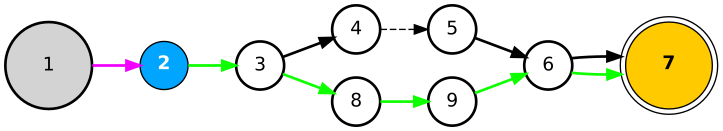
\includegraphics[width=\textwidth]{figuras/mapa_etapa3.png}
	\caption{Trajeto esperado do cenário 3 do experimento.}
	\label{fig:mapa_etapa3}
\end{figure}

Os três cenários desse experimento foram realizados em dois \textit{laptops} com 8 CPUs virtuais (1.80 GHz) e 8 GB de memória RAM.
Diferente do experimento apresentado na Seção \ref{sec:exp_smart_parking}, o foco desse experimento não é analisar o desempenho da plataforma, mas sim uma análise funcional. 
Os passos para execução desse experimento de validação foram os seguintes:

\begin{enumerate}
    \item Executar uma instância em modo de produção da plataforma InterSCity em um \textit{laptop}.

    \item Executar uma instância em modo de produção do simulador InterSCSimulator no outro \textit{laptop}.

    \item Configurar rede local entre os \textit{laptops}, conectados de maneira cabeada via ethernet.

    \item Realizar a simulação do cenário de tráfego inteligente de carros.

    \item Analizar os resultados obtidos ao final da simulação.
\end{enumerate}

A Figura \ref{fig:distancia_validacao}, apresenta a distância média percorrida pelos carros simulados nos três cenários deste experimento.
De acordo com as nossas hipóteses, esperávamos que os carros no cenário sem evento de fechamento de via e sem PMV para notificar os motoristas, percorressem 6 arestas, no cenário com evento e sem PMV
percorressem 8 arestas e no cenário com evento e PMV percorressem entre 6 e 8 arestas (alguns veículos ignoram as notificações).
Nossas hipóteses foram confirmadas, conforme o gráfico.

\begin{figure}[ht]
	\centering
	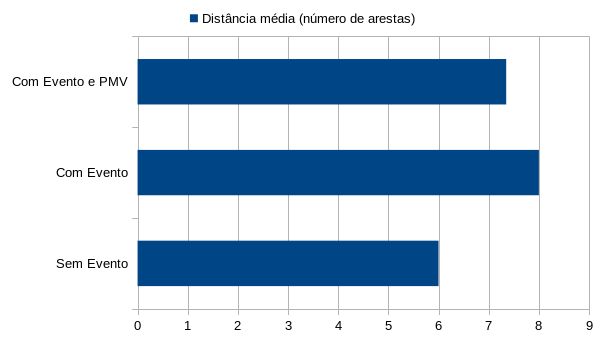
\includegraphics[width=\textwidth]{figuras/distancia_validacao.png}
	\caption{Média da distância percorrida pelos carros no experimento.}
	\label{fig:distancia_validacao}
\end{figure}

Uma análise semelhante foi realizada com a duração das viagens simuladas, como pode ser visto na Figura \ref{fig:duracao_validacao}.
As durações média das viagens simuladas nos três cenários do experimento são apresentadas no gráfico.
Uma viagem dura sempre 2 ciclos de execução (criação e destruição do ator) mais o tempo utilizado para percorrer as arestas (uma aresta por ciclo de execução, já que possuem comprimento unitário)
e o recálculo de um caminho dura um ciclo.
Por isso, esperávamos que para o cenário sem evento de fechamento de via durasse 8 ciclos (2 pelo ciclo de vida + 6 arestas);
o cenário com evento e sem PMV, para informar os motoristas, durasse 11 ciclos (2 pelo ciclo de vida + 8 arestas + 1 pelo recálculo da rota);
e o cenário com evento e PMV durasse entre 9 ciclos (2 pelo ciclo de vida + 6 arestas + 1 pelo recálculo) para motoristas que seguissem as instruções da PMV, e 11 ciclos (2 pelo ciclo de vida + 8 arestas +
1 pelo recálculo) para os motoristas que ignorassem a PMV.
Nossas hipóteses mais uma vez foram confirmadas, como pode ser visto na Figura \ref{fig:duracao_validacao}.

\begin{figure}[ht]
	\centering
	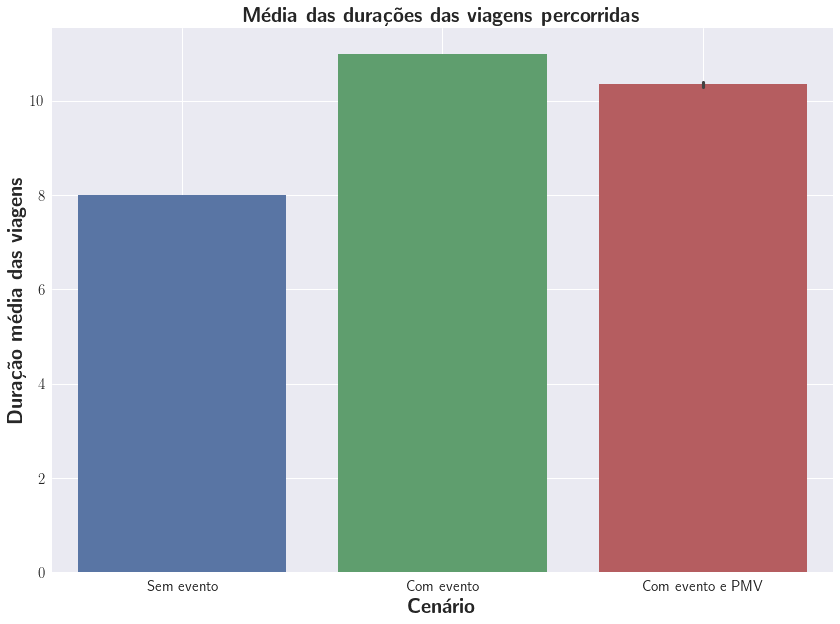
\includegraphics[width=\textwidth]{figuras/duracao_validacao.png}
	\caption{Média da duração das viagens simuladas no experimento.}
	\label{fig:duracao_validacao}
\end{figure}

Com isso, pudemos verificar os requisitos fundamentais e de integração, apresentados na Seção \ref{sec:requisitos}, para este cenário de tráfego de carros inteligentes.
O modelo implementado no simulador correspondeu com o esperado e a comunicação entre as ferramentas foi validada, principalmente com o que diz respeito à atuação no ambiente simulado, sendo esse um
trabalho pioneiro.

\subsubsection{Cidade de São Paulo}
\label{sec:smart_traffic}

Tendo em vista que a implementação dos modelos utilizados para este cenário e a integração estavam funcionando dentro do esperado, realizamos um outro experimento, envolvendo o mesmo cenário de tráfego 
inteligente de carros, mas dessa vez em uma escala maior, com dados abertos da cidade de São Paulo.

Dividimos esse experimento em três cenários novamente, quanto ao número de eventos de fechamento de via e PMVs. Eles se deram da seguinte forma:

\begin{enumerate}
    \item Sem eventos de fechamento de via e sem PMVs

    \item Com eventos de fechamento de via e sem PMVs

    \item Com eventos de fechamento de via e 7 PMVs
\end{enumerate}

Foram executadas 20 iterações de cada uma dos cenários e, em cada iteração, simulamos 1 hora e 30 minutos.
Neste experimento, utilizamos dados do OpenStreet Maps e a pesquisa Origem-Destino realizado pela companhia de metrô da cidade de São Paulo em 2007 para definição do cenário a ser simulado.
A seguir mais detalhes sobre esses dados.

Dessa vez, não utilizamos o mapa viário completo da cidade de São Paulo.
Realizamos um recorte de um trecho da avenida Rebouças com um raio de 5km, próximo ao cruzamento da avenida Paulista.
O intuito desse recorte era reduzir o escopo do experimento para enfatizar o impacto das PMVs naquela região.
Para a criação das viagens de carros a serem realizadas, utilizamos os mesmos dados da pesquisa OD (Origem-Destino) apresentada no experimento de estacionamento inteligente.
Contudo, como não utilizamos o mapa completo da cidade, filtramos apenas as viagens em que a origem e o destino pertencessem ao recorte do mapa realizado.
Todos os \textit{scripts} utilizados para filtrar os dados de entrada estão disponíveis em nosso repositório aberto\footnote{https://github.com/LSS-USP/pmv\_experiment}.

\begin{itemize}
    \item \textbf{OpenStreet Maps}: para criar o grafo viário da cidade de São Paulo usado na simulação, utilizamos o mapa do OpenStreet Maps.
        Este mapa contém todas as ruas e junções da cidade, em conjunto com um vasto número de atributos, como comprimento, capacidade e velocidade limite.
        Tais informações são usadas pelo simulador para definir as rotas percorridas pelos carros durante a realização de suas viagens, bem como simular o impacto do tráfego na velocidade dos carros.

    \item \textbf{Pesquisa Origem-Destino (OD)}: criamos as viagens de carro simuladas com base na pesquisa OD realizada pela Companhia de Metrô de São Paulo.
        \footnote{Pesquisa Origem-Destino - http://goo.gl/Te2SX7.}
        Essa pesquisa descreve as viagens de 200.000 pessoas e extrapola os dados para toda a população da cidade.
        A pesquisa inclui informações sobre a origem, o destino, o modo de transporte e a hora de partida.
        Esses dados foram empregados para definir o comportamento dos agentes do tipo carro na simulação.
        Simulamos o tráfego em São Paulo durante o horário das 8h às 9h30.
        Na pesquisa OD, há 2.210 viagens de carro que começam durante o intervalo de tempo considerado e no recorte do mapa feito.
\end{itemize}

No cenário 3 deste experimento, onde fizemos uso de 7 PMVs, posicionamos os mesmos nas principais vias presentes no recorte do mapa, como pode ser visto na Figura \ref{fig:pos_pmvs}.
Decidimos sinalizar tais vias acreditando que por possuírem um maior fluxo de carros, possivelmente impactariam nas rotas de mais carros.

\begin{figure}[ht]
	\centering
	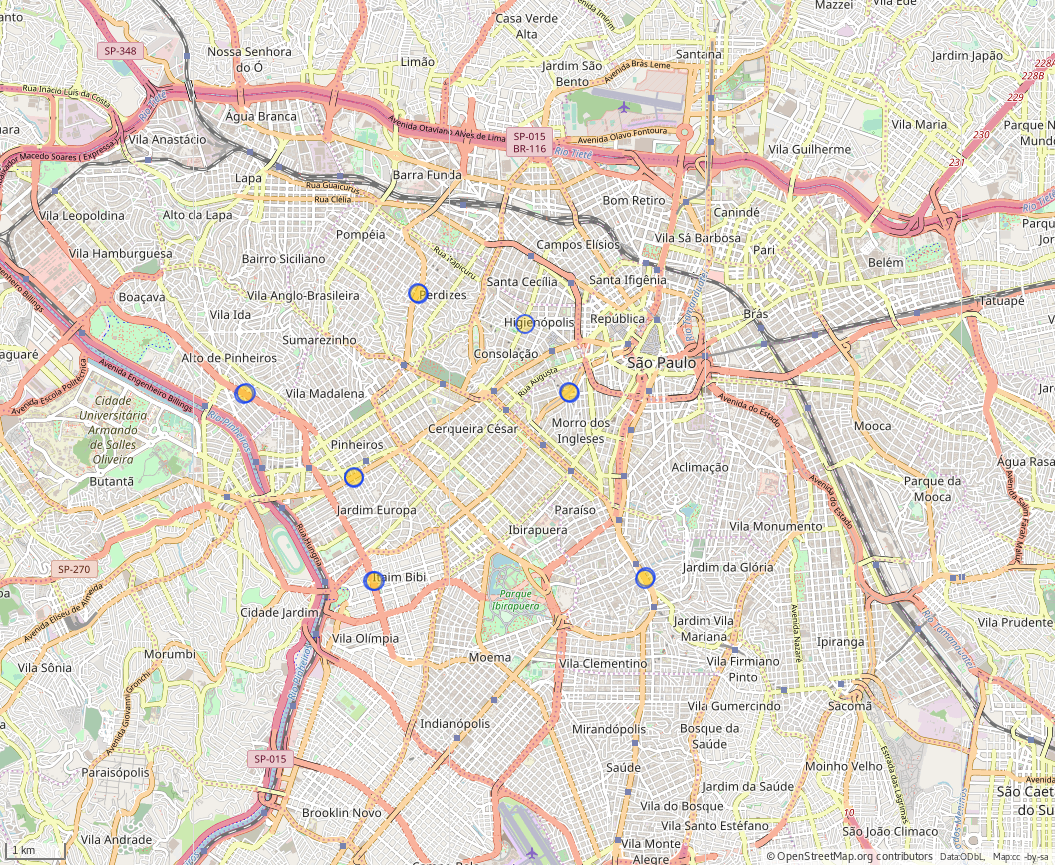
\includegraphics[width=.7\textwidth]{figuras/pmvs_locations.png}
	\caption{Posicionamento das PMVs no experimento de tráfego inteligente de carros.}
	\label{fig:pos_pmvs}
\end{figure}

Na Figura \ref{fig:eventos}, pode-se ver os trechos de vias que foram fechadas nos cenários 2 e 3 deste experimento.
No grafo do mapa viário da cidade gerado a partir do OpenStreet Maps, uma mesma via é formada de várias pequenas arestas (segmentos de via).
Visando enfatizar um evento como um acidente de carro fatal ou um possível alagamento na região, fechamos um conjunto de arestas nas proximidades das avenidas Rebouças e Paulista.

\begin{figure}[ht]
	\centering
	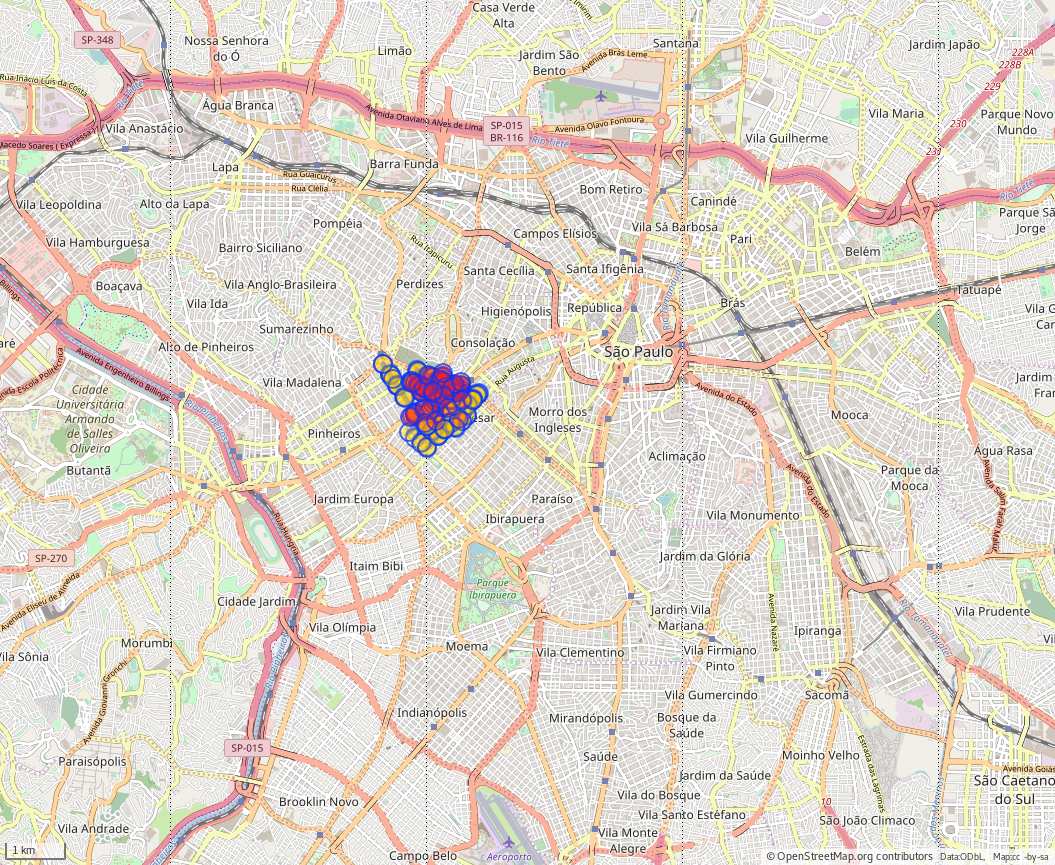
\includegraphics[width=.7\textwidth]{figuras/events_edges_map.png}
	\caption{Local dos eventos de fechamento de via no experimento de tráfego de carros inteligente.}
	\label{fig:eventos}
\end{figure}

Sabendo o local dos eventos de fechamento de vias e o posicionamento das PMVs, esperávamos que a notificação prévia dos motoristas sobre o acidente reduzisse a média do tempo de viagem dos motoristas
com relação a não existência das PMVs.
Consideramos que, pelo fato das avenidas Rebouças e Paulista serem bem movimentadas, muitas das viagens simuladas neste experimento passassem por aquele trecho. 
Contudo, a utilização das PMVs não deveria melhorar a média da duração das viagens em relação ao cenário onde não acontece nenhum evento de fechamento de via.

Os três cenários desse experimento foram realizadas novamente em dois \textit{laptops} com 8 CPUs virtuais (1.80 GHz) e 8 GB de memória RAM.
Mais uma vez, diferente do experimento apresentado na Seção \ref{sec:exp_smart_parking}, o foco desse experimento não é analisar o desempenho da plataforma, mas sim uma análise funcional. 
Os passos para execução desse experimento foram os seguintes:

\begin{enumerate}
    \item Executar uma instância em modo de produção da plataforma InterSCity em um \textit{laptop}.

    \item Executar uma instância em modo de produção da simulador InterSCSimulator no outro \textit{laptop}.

    \item Configurar rede local entre os \textit{laptops}, conectados de maneira cabeada via ethernet.

    \item Realizar a simulação do cenário de tráfego de carros inteligente.

    \item Analizar os resultados obtidos ao final da simulação.
\end{enumerate}

A Figura \ref{fig:duracao_total}, apresenta a duração média das viagens de carro simuladas nos três cenários deste experimento.
No eixo X, a duração é apresentada em segundos (ciclo de execução da simulação: 1 ciclo = 1 segundo), e no eixo Y os três cenários do experimento.
Como podemos ver no gráfico apresentado, em geral, a média do tempo de duração das viagens não passou de 6 minutos.
Isso pode ter ocorrido pelo fato das viagens nessa região serem mais curtas, ou por não terem viagens suficientes para gerar congestionamentos, já que filtramos apenas as viagens que se iniciavam e
terminavam dentro do recorte do mapa utilizado.
Outro fator importante que nos chamou a atenção, foi a média da duração das viagens do cenários 3 (onde existem vias fechadas e o auxilio de PMVs) ser menor do que do cenário 1 (onde não existe qualquer
incidente).
Após analisar os dados, percebemos que ao recalcular a rota, na presença de uma PMV, os carros se distribuíam de uma melhor forma pela malha viária do cenário utilizado pelo experimento, com isso,
evitavam congestionamentos que ocorriam anteriormente.
Sendo isso um alvo de possível melhoria no simulador, já que ao criar o ator, apenas um dos menores caminhos entre a origem e destino do carro é calculado e utilizado, podendo essa rota coincidir entre
múltiplos atores com origem e destinos similares, assim, deixando outros caminhos mais curtos inutilizados.
Todavia, como esperado, o cenário 2, onde temos fechamento de vias mas não temos PMVs, teve a maior média de duração das viagens.

\begin{figure}[ht]
	\centering
	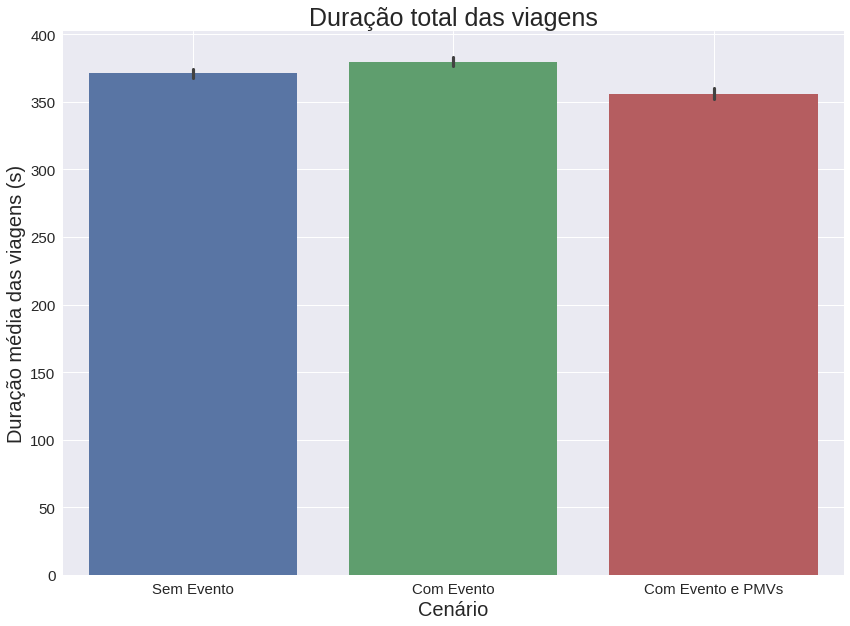
\includegraphics[width=\textwidth]{figuras/duracao_total.png}
	\caption{Média da duração das viagens de carros no experimento.}
	\label{fig:duracao_total}
\end{figure}

Para garantirmos uma melhor acurácia na análise dos resultados obtidos, filtramos apenas as viagens que foram influencidas de alguma forma pelo fechamento de vias e/ou PMVs.
Isso porque percebemos a existência de viagens que não eram modificadas em nenhum dos cenários do experimento, ou seja, a sua duração era sempre a mesma.
Na Figura \ref{fig:duracao_filtered}, apresentamos o mesmo gráfico discutido anteriormente, só que incluindo apenas as viagens que foram afetadas.
Agora analisando o gráfico com as viagens afetadas, obtivemos o resultado esperado no início do experimento.
O cenário 1, onde não há vias fechadas, teve o menor tempo médio de duração de viagens, sendo esse o nosso limite inferior.
O cenário 2, onde vias foram fechadas, o pior tempo médio de viagem foi obtido, sendo o limite superior.
E o cenário 3, onde introduzimos as PMVs para auxiliar os motoristas na decisão da melhor rota a seguir, apresentou um tempo médio de viagem ligeiramente menor do que o cenário 2 e maior do que o cenário 1.

\begin{figure}[ht]
	\centering
	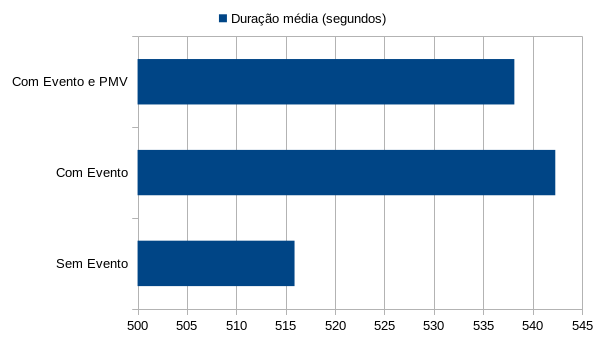
\includegraphics[width=\textwidth]{figuras/duracao_filtered.png}
	\caption{Média da duração das viagens de carros afetadas por fechamento de vias e/ou PMVs no experimento.}
	\label{fig:duracao_filtered}
\end{figure}

Contudo, a melhora de aproximadamente 5\% na média do tempo de duração da viagem do cenário 3 com relação ao cenário 2 não foi um resultado expressivo.
Avaliamos que alguns fatores podem ter influenciado nesse resultado, sendo a maioria deles voltado para os dados utilizados para a definicação do cenário de simulação deste experimento.
O posicionamento das PMVs pode não ter sido o ideal, já que não foi realizada uma análise prévia de onde passariam a maior parte dos carros.
O conjunto de viagens simulados após recortar o mapa da cidade de São Paulo pode não ter sido representativo, a decisão de reduzir o mapa para facilitar a visualização do impacto do fechamento de vias
e PMVs pode não ter sido boa ideia.
Além disso, os resultados obtidos podem ter sido influenciados devido à infraestrutura simples utilizada com apenas dois \textit{laptops}, já que em cenários realistas muitos recursos computationais são
necessários, como memória e largura de banda da rede.


\section{Discussão}

% Melhorias, o que fucionou, o que não funcionou

Após a realização dos dois estudos de caso apresentados neste capítulo, foi possível perceber que a solução proposta no Capítulo \ref{cap:proposta} é viável e nos permitiu realizar
diferentes experimentos utilizando um ambiente simulado de uma cidade, podendo substituir \textit{testbeds} reais e aumentando a escala dos experimentos.
Contudo, durante a implementação dos dois cenários de Cidades Inteligentes apresentados, algumas adversidades foram encontradas e solucionadas.
A fim de contribuir com trabalhos futuros que sigam a solução proposta, uma discussão sobre os principais problemas e dificuldades encontradas será feita
nesta seção.
O intuito aqui é enfatizar os principais obstáculos a serem enfrentados durante a implementação de novos cenários no ambiente integrado usando o simulador InterSCSimulator e
a plataforma InterSCity ou até mesmo envolvendo outras ferramentas, bem como discutir os resultados experimentais alcançados nos estudos de caso.


\subsection{Implementação da Solução Proposta}

Como vem sendo discutido no decorrer deste trabalho, a integração de ferramentas não é algo trivial.
Apesar de tanto o simulador quanto a plataforma utilizada serem voltados para o contexto de Cidades Inteligentes, na maioria das vezes, elas não são concebidas inicialmente
para serem integradas com outras ferramentas.
Através dos próprios requisitos apresentados podemos antever o maior desafio a ser enfrentado: a interoperabilidade.
Essa tanto a nível de comunicação quanto semanticamente.

Como constatado na implementação dos dois cenários apresentados, tentamos ao máximo reduzir a responsabilidade do componente de integração, que ao ser atribuído muitas
tarefas pode se tornar um problema.
Tanto que não foi necessária a implementação desse componente no segundo estudo de caso, tendo em vista que as ferramentas já atendiam os requisitos de integração.
Isso pode ser atribuído ao fato de ambas as ferramentas (InteSCSimulator e InterSCity) serem mantidas pelo nosso grupo de pesquisa, onde tivemos a liberdade de evoluir o
que foi preciso nas próprias ferramentas para facilitar a integração.
Em um contexto onde não existisse essa flexibilidade, o desafio se tornaria bem mais complexo.

Mesmo assim, enfrentamos problemas principalmente com a escalabilidade da solução.
Em experimentos anteriores e isolados, foi demonstrado que ambas as ferramentas eram escaláveis, se comportando bem diante de uma grande carga de trabalho.
Entretanto, a integração traz alguns elementos extras que, por menor que sejam, interferem em cenários de larga escala.
Em experimentos na escala de uma cidade como São Paulo, qualquer mínimo detalhe é potencializado.
Semanticamente não tivemos muitos problemas, já que ambas as ferramentas foram implementadas seguindo conceitos similares, devido a própria sinergia do grupo de
pesquisa.
Todavia, a comunicação entre as ferramentas foi a raíz da maior parte dos problemas enfrentados.

Inicialmente, tentamos realizar qualquer interação com a plataforma através de requisições HTTP, usando a sua API \textit{Restful}.
Contudo, percebemos que o componente de integração necessitaria de uma complexidade muito maior para tratar todas essas requisições paralelamente sem se tornar um
gargalo para o sistema.
Por isso, decidimos explorar bastante o protocolo AMQP através da implementação do RabbitMQ.
Essa se apresentou uma solução mais simples, já que o \textit{broker} do RabbitMQ trata todas essas questões de escalabilidade de maneira eficiente, sendo essa
uma solução adotada pelo mercado.
Além do mais, pelo fato da comunicação via AMQP ser assíncrona e pela própria natureza dos cenários implementados, diferente de requisições HTTP, ela se apresentou uma
solução mais adequada, não bloqueando agentes da simulação a espera de respostas.
Logo, sempre que possível, transferir responsabilidades para ferramentas de terceiros comprovadamente capazes de atender os requisitos ao invés de implementar a sua
própria solução, é desejável.

Nesse processo de melhoria da escalabilidade da solução integrada, várias mudanças foram feitas em ambas as ferramentas.
Foram encontrados problemas de escalabilidade antes não evidenciados por outros experimentos isolados, demonstrando que a solução de ambiente de experimentação para
plataformas de Cidades Inteligentes atingiu seus objetivos, apontando melhorias nos sistemas que só seriam evidenciadas ao enfrentar cargas de trabalho da magnitude de uma
cidade como São Paulo.

Na plataforma InterSCity, implementações envolvendo técnicas para armazenamento em cache de dados mais utilizados foram feitas.
Ademais, melhorias envolvendo a automatização da implantação da plataforma foram realizadas.
Já no InterSCSimulator, encontramos alguns problemas na implementação dos modelos apresentados que causaram problemas de escalabilidade.
Ou seja, dependendo do cenário e de como foi implementado, apenas reduzir a complexidade do componente de integração (até mesmo a não existência) ainda não é a solução.
Portanto, poder modificar as próprias ferramentas é algo interessante, haja vista que a forma em que os modelos, métodos e funcionalidades foram implementados podem não
ter sido testados em ambientes de estresse, tornando-se gargalos durante experimentos de larga escala.
Isso evidencia a importância da utilização de ferramentas livres para a construção de ambientes de experimentação para plataformas de Cidades Inteligentes.


\subsection{Experimentos}

Um ponto importante para a realização de experimentos, e ainda mais envolvendo múltiplas ferramentas, é a automatização desse processo.
Tal automatização facilita a execução de várias rodadas do experimento e a reprodução do trabalho por terceiros.
Neste trabalho, acreditamos que ambos os estudos de caso foram devidamente automatizados e documentados, favorecendo a continuidade do trabalho.

No primeiro estudo de caso conseguimos evidenciar a escalabilidade horizontal da plataforma InterSCity.
Várias melhorias foram realizadas e gargalos solucionados, o que nos demonstrou a extrema importância da realização desse tipo de experimento durante o ciclo de desenvolvimento de plataformas de Cidades
Inteligentes.
Já no segundo estudo de caso, demonstramos a viabilidade da atuação em tempo de execução em um ambiente simulado, sendo esse um trabalho pioneiro na área de Cidades Inteligentes.
 
Contudo, como o foco principal do trabalho é prover uma solução de ambiente simulado para a realização de experimentos em plataformas de Cidade Inteligentes, acreditamos que algumas das análises
apresentadas nos estudos de caso poderiam ser melhoradas.
Ademais, especialmente no segundo estudo de caso, algumas decisões iniciais do experimento poderiam ter sido otimizadas, como o posicionamento das PMVs baseado em uma análise mais profunda da movimentação
dos carros nas viagens selecionadas para o experimento, o que prejudicou os resultados obtidos.
A utilização de \textit{laptops} para a execução do segundo experimento também contribuiu para o resultado final abaixo do esperado, tendo em vista que esse tipo de experimento requer muitos recursos
computacionais.

Em resumo, os estudos de caso foram satifatórios, já que foi possível validar a proposta de solução em dois cenários de Cidades Inteligentes distintos, exercitando as principais funcionalidades que
um ambiente de experimentação simulado deve possuir.



\par

\chapter{Conclusão}
\label{cap:conclusao}

%Proposta de integração de plataforma e simulador para prover o ambiente de
%experimentação
%
%Viabilidade da proposta através de dois estudos de caso
%
%Ambiente de experimentação emulado é uma opção diante da necessidade de
%avaliaçãoes dessas plataformas em larga-escala
%
%Artigos publicados/a serem publicados

A proposta de arquitetura para criação de um ambiente simulado de experimentação para plataformas de Cidades Inteligentes apresentou-se como uma solução viável, tendo em vista que fomos capazes de
realizar experimentos de diferentes naturezas utilizando implementações feitas a partir da sistematização guiada pela solução pensada.
Durante a pesquisa, percebemos que a utilização de simulação é uma saída para a realização de experimentos na escala de grandes cidades, sem a necessidade de muitos investimentos em \textit{testbeds} reais.
A experimentação de tecnologias ainda não difundidas ou até mesmo inexistentes, como por exemplo o uso de Placas de Mensagens Variadas (PMVs) notificando motoristas
em tempo real sobre problemas no trânsito, carros autônomos, estacionamentos inteligentes, dentre outros nos aproximou da realidade, fazendo-nos acreditar nas diversas possibilidades quanto ao
investimento na pesquisa de Cidades Inteligentes.

Concluímos também que a tarefa de criar um ambiente de experimentação envolvendo a integração de ferramentas não é trivial, corroborando com a literatura.
Apesar de ambas as ferramentas utilizadas para implementação da arquitetura proposta serem desenvolvidas pelo nosso grupo de pesquisa, encontramos diversos entraves durante o processo.
Esses problemas nos mostraram a importância da utilização de ferramentas de código aberto, pois muitas vezes o componente de integração, introduzido pela nossa proposta de solução, não é capaz de
solucionar problemas inerentes as ferramentas.
Problemas esses que, em geral, são evidenciados somente em cenários similares ao contexto enfrentado por metrópoles, demonstrando a importância da realização desse tipo de experimento durante o ciclo de
desenvolvimento de plataformas para Cidades Inteligentes.

Ademais vimos que, apenas a existência de um ambiente simulado que permita a realização de experimentos em escalas maiores não soluciona todos os problemas, é necessário a definição precisa do cenário
de simulação através de dados reais de cidades, portanto, esse elemento é de suma relevância.
Como apresentado na Seção \ref{sec:smart_traffic}, os resultados obtidos no segundo estudo de caso não foram melhores devido o não conhecimento detalhado dos dados de entrada utilizados.
Outro ponto importante na realização de experimentos é a automatização desse processo, contribuindo com trabalhos que possam ser derivados através da reprodução dos mesmos, fazendo uso de ferramentas
e técnicas de infraestrutura como código (IaC).

Por fim, utilizando o ambiente de experimentação simulado desenvolvido neste trabalho, publicamos o artigo \textit{Design and evaluation of a scalable smart city software platform with
large-scale simulations}\footnote{https://www.sciencedirect.com/science/article/pii/S0167739X18307301} juntamente com colegas do nosso grupo de pesquisa, na revista \textit{Future Generation of
Computer Systems} edição 93 que será publicada em abril de 2019.  
Essa publicação em uma revista bem conceituada foi de suma importância para demostrarmos que a abordagem apresentada neste estudo é factível e inovadora na área de Cidades Inteligentes.


\section{Limitações do trabalho}

%Arquitetura depende das ferramentas suportarem os protocolos apresentados

A primeira limitação identificada é o fato da proposta de solução apresentada não ter sido validada com outras ferramentas além do InterSCSimulator e da InterSCity.
Essa validação seria interessante para reafirmarmos que a solução proposta tem um âmbito genérico, contemplando quaisquer ferramentas.
Ainda sobre a arquitetura de integração, não tivemos a oportunidade de implementar um módulo de tradução semântica, já que ambas as ferramentas tinham conceitos similares implementados.
Sabemos que o mesmo é de suma importância em casos onde as ferramentas não são desenvolvidas pelo mesmo grupo de pessoas.

Além disso, os estudos de casos apresentam algumas limitações, principalmente o que contempla o cenário de tráfego de carros inteligente.
Como já foi dito, as entradas para a simulação deveriam ter sido melhor analisadas previamente, o que desencadeou a não obtenção de resultados mais expressivos.
Todavia, acreditamos que apesar dessa limitação, o estudo de caso cumpriu o seu papel que era verificar a viabilidade de execução de experimentos fazendo uso de comandos de atuação no
ambiente simulado.

\section{Trabalhos Futuros}

%Integração de novos cenários de cidades inteligentes seguindo a proposta de
%solução apresentada (InterSCity + InterSCSimulator)
%
%Implementar a solução proposta utilizando outras ferramentas (plataforma e
%simulador/emulador)
%
%Implementar a solução proposta utilizando outros protocolos de rede (MQTT, web
%sockets, ...)

Para a continuidade deste trabalho seria interessante a utilização de diferentes ferramentas para a implementação da solução proposta.
Ao utilizar uma plataforma e um simulador diferente, poderíamos validar a arquitetura apresentada em um contexto diferente, principalmente com o que diz respeito ao componente de integração, que provavelmente
necessitará de um módulo de tradução semântica e mais complexidade embutida em sua implementação.

Nesse sentido, também seria interessante adicionar novos cenários de Cidades Inteligentes no ambiente já integrado neste trabalho, com o InterSCSimulator e a InterSCity, e realizar novos experimentos.
Como foi visto no decorrer da dissertação, novos cenários trazem novos desafios e, portanto, requisitos fundamentais que eventualmente necessitam ser implementados ou evoluídos dentro das ferramentas 
mencionadas.
Quanto mais cenários de Cidades Inteligentes ao ambiente de experimentação InterSCSimulator + InterSCity nós adicionarmos, mais interessante se tornará a nossa solução, além de estarmos avaliando a
plataforma InterSCity constantemente em condições realistas.

A utilização de outros protocolos de rede para realizar a comunicação entre o simulador e a plataforma também seria algo interessante.
Neste trabalho utilizamos apenas os protocolos HTTP e AMQP nas implementações dos dois cenários de Cidades Inteligentes, foco do estudo.
Protocolos como o MQTT\footnote{http://mqtt.org/} e CoAP\footnote{http://coap.technology/} vem sendo amplamente utilizados para a comunicação com dispositivos IoT, conforme as diversas implementações de
plataformas desse tipo.

\par


\par


%%%%%%%%%%%%%%%%%%%%%%%%%%%%%%%% APÊNDICES %%%%%%%%%%%%%%%%%%%%%%%%%%%%%%%%%%%%%

% Aqui vão apêndices. O comando appendix reinicia a numeração de capítulos e
% passa a numerá-los com letras. Como os anteriores, ele não existe na classe
% "article".
\appendix

% Os apêndices podem ser inseridos diretamente aqui ou "puxados" de outros
% arquivos
\chapter{Código-Fonte e Pseudocódigo}
\label{ap:pseudocode}

Com a \textit{package} \textsf{listings}, programas podem ser inseridos
diretamente no arquivo, como feito no caso do Programa~\ref{prog:java},
ou importados de um arquivo externo com o comando
\textsf{\textbackslash{}lstinputlisting}, como no caso
do Programa~\ref{prog:mdcinput}.

% O exemplo foi copiado da documentação de algorithmicx
\begin{program}
  \lstinputlisting[
    language=pseudocode,
    style=pseudocode,
    style=wider,
    functions={},
    specialidentifiers={},
  ]
  {conteudo/euclid.psc}

  \caption{Máximo divisor comum (arquivo importado).\label{prog:mdcinput}}
\end{program}

Trechos de código curtos (menores que uma página) podem ou não ser
incluídos como \textit{floats}; trechos longos necessariamente incluem
quebras de página e, portanto, não podem ser \textit{floats}. Com
\textit{floats}, a legenda e as linhas separadoras são colocadas pelo
comando \textsf{\textbackslash{}begin\{program\}}; sem eles, utilize
o ambiente \textsf{ruledcaption} (atenção para a colocação do comando
\textsf{\textbackslash{}label\{\}}, dentro da legenda), como no
Programa~\ref{prog:mdc}\footnote{\textsf{listings} oferece alguns
recursos próprios para a definição de \textit{floats} e legendas, mas
neste modelo não os utilizamos.}:

\begin{ruledcaption}{Máximo divisor comum.\label{prog:mdc}}
  \begin{lstlisting}[
    language=pseudocode,
    style=pseudocode,
    style=wider,
    functions={},
    specialidentifiers={},
  ]
      function euclid($a,b$) // The \textbf{g.c.d.} of $a$ and $b$
          $r \gets a \bmod b$
          while $r \neq 0$ // We have the answer if $r$ is 0
              $a \gets b$
              $b \gets r$
              $r \gets a \bmod b$
          end
          return $b$ // The \textbf{g.c.d.} is $b$
      end
  \end{lstlisting}
\end{ruledcaption}

Além do suporte às várias linguagens incluídas em \textsf{listings},
este modelo traz uma extensão para permitir o uso de pseudocódigo,
útil para a descrição de algoritmos em alto nível. Ela oferece
diversos recursos:

\begin{itemize}

    \item É possível acrescentar palavras-chave com a opção
          ``\textsf{morekeywords=\{pchave1,\linebreak[0]{}pchave2\}}''
          (para um código específico) ou com o comando
          \textsf{\textbackslash{}lstset\{morekeywords=\linebreak[0]{}\{pchave1,pchave2\}\}}
          (como comando de configuração geral).

    \item É possível usar pequenos trechos de texto, como nomes de variáveis,
          dentro de um parágrafo normal com \textsf{\textbackslash{}lstinline\{blah\}}.

    \item Comentários seguem o padrão de C++ (\lstinline{//} e
          \lstinline{/* ... */}).

    \item ``\$\dots\$'' ativa o modo matemático em qualquer lugar.

    \item Outros comandos LaTeX funcionam apenas em comentários; fora, a
          linguagem simula alguns pré-definidos (\textsf{\textbackslash{}textit\{\}},
          \textsf{\textbackslash{}texttt\{\}} etc.).

    \item O comando \textsf{\textbackslash{}label} também funciona em
          comentários; a referência correspondente (\textsf{\textbackslash{}ref})
          indica o número da linha de código. Se quiser usá-lo numa linha sem
          comentários, use \lstinline{///}~\textsf{\textbackslash{}label\{blah\}};
          ``\lstinline{///}'' funciona como \lstinline{//}, permitindo
          a inserção de comandos \LaTeX{}, mas não imprime o delimitador
          (\ensuremath{\triangleright}).

    \item Para suspender a formatação automática, use \textsf{\textbackslash{}noparse\{blah\}}.

    \item Para forçar a formatação de um texto como função, identificador,
          palavra-chave ou comentário, use \textsf{\textbackslash{}func\{blah\}},
          \textsf{\textbackslash{}id\{blah\}}, \textsf{\textbackslash{}kw\{blah\}} ou
          \textsf{\textbackslash{}comment\{blah\}}.

    \item Palavras-chave dentro de comentários não são formatadas
          automaticamente; se necessário, use \textsf{\textbackslash{}func\{\}},
          \textsf{\textbackslash{}id\{\}} etc. ou comandos \LaTeX{} padrão.

    \item As palavras ``Program'', ``Procedure'' e ``Function'' têm formatação
          especial e fazem a palavra seguinte ser formatada como função.
          Funções em outros lugares \emph{não} são detectadas automaticamente;
          use \textsf{\textbackslash{}func\{\}}, a opção ``\textsf{functions=\{func1,func2\}}''
          ou o comando ``\textsf{\textbackslash{}lstset\{functions=\{func1,func2\}\}}''
          para que elas sejam detectadas.

    \item Além de funções, palavras-chave, strings, comentários e
          identificadores, há ``\textsf{specialidentifiers}''. Você pode
          usá-los com \textsf{\textbackslash{}specialid\{blah\}}, com a opção
          ``\textsf{specialidentifiers=\{id1,id2\}}'' ou com o comando
          ``\textsf{\textbackslash{}lstset\{specialidentifiers=\{id1,id2\}\}}''.

\end{itemize}



\par

\par


%%%%%%%%%%%%%%%%%%%%%%%%%%%%%% SEÇÕES FINAIS %%%%%%%%%%%%%%%%%%%%%%%%%%%%%%%%%%%

% Aqui vão a bibliografia, índice remissivo e outras seções similares.
% O comando backmatter desabilita a numeração de capítulos e também não existe
% na classe "article".
\backmatter

% Este formato está definido mais acima na seção "APARÊNCIA/FORMATAÇÃO"
\pagestyle{frontback}

\singlespacing   % espaçamento simples

% A bibliografia é obrigatória

%%%%%%%%% Bibliografia com natbib (preterido): %%%%%%%%%
%\bibliographystyle{alpha-ime}% citação bibliográfica alpha
%\bibliographystyle{plainnat-ime} % citação bibliográfica textual
%\bibliography{bibliografia}  % associado ao arquivo: 'bibliografia.bib'

%%%%%%%% Bibliografia com biblatex (preferido): %%%%%%%%

\printbibliography[
  title=Bibliografia\label{bibliografia},
  % Inclui a bibliografia no sumário; comente se estiver usando "article"
  heading=bibintoc,
]

% imprime o índice remissivo no documento (opcional)
\printindex

\end{document}
